% Created by tikzDevice version 0.8.1 on 2015-12-07 17:04:15
% !TEX encoding = UTF-8 Unicode
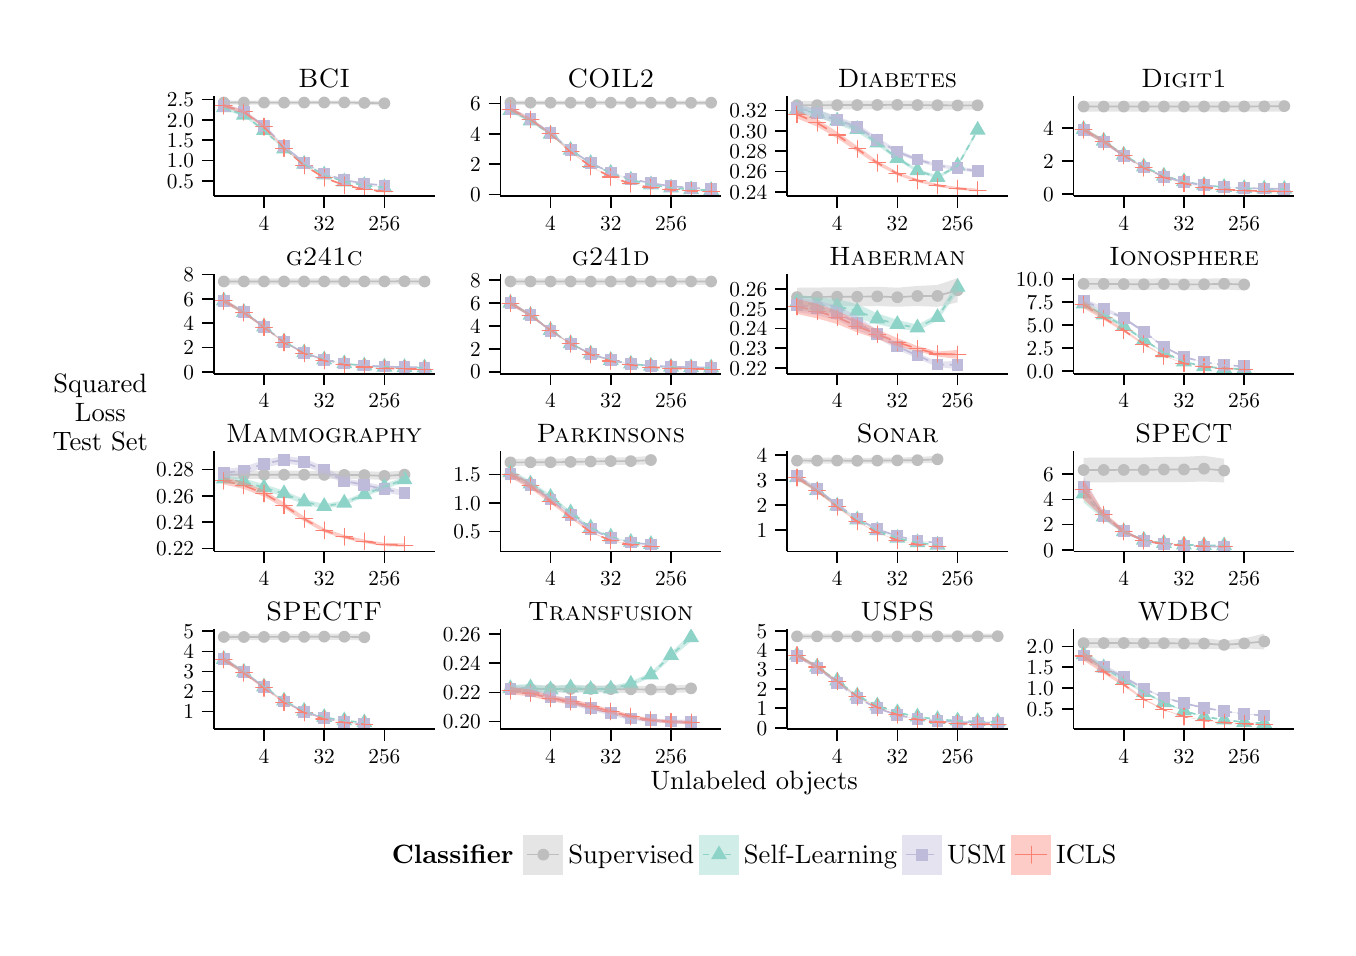
\begin{tikzpicture}[x=1pt,y=1pt]
\definecolor{fillColor}{RGB}{255,255,255}
\path[use as bounding box,fill=fillColor,fill opacity=0.00] (0,0) rectangle (469.75,325.21);
\begin{scope}
\path[clip] (  0.00,  0.00) rectangle (469.75,325.21);
\definecolor{drawColor}{RGB}{255,255,255}
\definecolor{fillColor}{RGB}{255,255,255}

\path[draw=drawColor,line width= 0.6pt,line join=round,line cap=round,fill=fillColor] (  0.00,  0.00) rectangle (469.76,325.21);
\end{scope}
\begin{scope}
\path[clip] ( 67.25,264.38) rectangle (147.04,300.54);
\definecolor{fillColor}{RGB}{255,255,255}

\path[fill=fillColor] ( 67.25,264.38) rectangle (147.04,300.54);
\definecolor{fillColor}{RGB}{190,190,190}

\path[fill=fillColor] ( 70.88,298.15) circle (  2.13);
\definecolor{fillColor}{RGB}{141,211,199}

\path[fill=fillColor] ( 70.88,299.62) --
	( 73.75,294.65) --
	( 68.01,294.65) --
	cycle;
\definecolor{fillColor}{RGB}{190,186,218}

\path[fill=fillColor] ( 68.75,294.86) --
	( 73.01,294.86) --
	( 73.01,299.13) --
	( 68.75,299.13) --
	cycle;
\definecolor{drawColor}{RGB}{251,128,114}

\path[draw=drawColor,line width= 0.4pt,line join=round,line cap=round] ( 67.86,297.03) -- ( 73.90,297.03);

\path[draw=drawColor,line width= 0.4pt,line join=round,line cap=round] ( 70.88,294.01) -- ( 70.88,300.04);
\definecolor{fillColor}{RGB}{190,190,190}

\path[fill=fillColor] ( 78.13,298.15) circle (  2.13);
\definecolor{fillColor}{RGB}{141,211,199}

\path[fill=fillColor] ( 78.13,296.98) --
	( 81.01,292.01) --
	( 75.26,292.01) --
	cycle;
\definecolor{fillColor}{RGB}{190,186,218}

\path[fill=fillColor] ( 76.00,292.81) --
	( 80.27,292.81) --
	( 80.27,297.08) --
	( 76.00,297.08) --
	cycle;

\path[draw=drawColor,line width= 0.4pt,line join=round,line cap=round] ( 75.12,294.83) -- ( 81.15,294.83);

\path[draw=drawColor,line width= 0.4pt,line join=round,line cap=round] ( 78.13,291.81) -- ( 78.13,297.84);
\definecolor{fillColor}{RGB}{190,190,190}

\path[fill=fillColor] ( 85.39,298.13) circle (  2.13);
\definecolor{fillColor}{RGB}{141,211,199}

\path[fill=fillColor] ( 85.39,291.46) --
	( 88.26,286.48) --
	( 82.51,286.48) --
	cycle;
\definecolor{fillColor}{RGB}{190,186,218}

\path[fill=fillColor] ( 83.25,287.56) --
	( 87.52,287.56) --
	( 87.52,291.83) --
	( 83.25,291.83) --
	cycle;

\path[draw=drawColor,line width= 0.4pt,line join=round,line cap=round] ( 82.37,289.41) -- ( 88.40,289.41);

\path[draw=drawColor,line width= 0.4pt,line join=round,line cap=round] ( 85.39,286.39) -- ( 85.39,292.43);
\definecolor{fillColor}{RGB}{190,190,190}

\path[fill=fillColor] ( 92.64,298.12) circle (  2.13);
\definecolor{fillColor}{RGB}{141,211,199}

\path[fill=fillColor] ( 92.64,284.80) --
	( 95.51,279.82) --
	( 89.77,279.82) --
	cycle;
\definecolor{fillColor}{RGB}{190,186,218}

\path[fill=fillColor] ( 90.51,280.27) --
	( 94.77,280.27) --
	( 94.77,284.54) --
	( 90.51,284.54) --
	cycle;

\path[draw=drawColor,line width= 0.4pt,line join=round,line cap=round] ( 89.62,281.68) -- ( 95.66,281.68);

\path[draw=drawColor,line width= 0.4pt,line join=round,line cap=round] ( 92.64,278.67) -- ( 92.64,284.70);
\definecolor{fillColor}{RGB}{190,190,190}

\path[fill=fillColor] ( 99.89,298.14) circle (  2.13);
\definecolor{fillColor}{RGB}{141,211,199}

\path[fill=fillColor] ( 99.89,279.25) --
	(102.77,274.27) --
	( 97.02,274.27) --
	cycle;
\definecolor{fillColor}{RGB}{190,186,218}

\path[fill=fillColor] ( 97.76,274.31) --
	(102.03,274.31) --
	(102.03,278.58) --
	( 97.76,278.58) --
	cycle;

\path[draw=drawColor,line width= 0.4pt,line join=round,line cap=round] ( 96.87,275.44) -- (102.91,275.44);

\path[draw=drawColor,line width= 0.4pt,line join=round,line cap=round] ( 99.89,272.42) -- ( 99.89,278.46);
\definecolor{fillColor}{RGB}{190,190,190}

\path[fill=fillColor] (107.15,298.17) circle (  2.13);
\definecolor{fillColor}{RGB}{141,211,199}

\path[fill=fillColor] (107.15,275.36) --
	(110.02,270.38) --
	(104.27,270.38) --
	cycle;
\definecolor{fillColor}{RGB}{190,186,218}

\path[fill=fillColor] (105.01,270.37) --
	(109.28,270.37) --
	(109.28,274.64) --
	(105.01,274.64) --
	cycle;

\path[draw=drawColor,line width= 0.4pt,line join=round,line cap=round] (104.13,271.00) -- (110.16,271.00);

\path[draw=drawColor,line width= 0.4pt,line join=round,line cap=round] (107.15,267.99) -- (107.15,274.02);
\definecolor{fillColor}{RGB}{190,190,190}

\path[fill=fillColor] (114.40,298.19) circle (  2.13);
\definecolor{fillColor}{RGB}{141,211,199}

\path[fill=fillColor] (114.40,272.88) --
	(117.27,267.90) --
	(111.52,267.90) --
	cycle;
\definecolor{fillColor}{RGB}{190,186,218}

\path[fill=fillColor] (112.26,268.01) --
	(116.53,268.01) --
	(116.53,272.28) --
	(112.26,272.28) --
	cycle;

\path[draw=drawColor,line width= 0.4pt,line join=round,line cap=round] (111.38,268.28) -- (117.42,268.28);

\path[draw=drawColor,line width= 0.4pt,line join=round,line cap=round] (114.40,265.26) -- (114.40,271.30);
\definecolor{fillColor}{RGB}{190,190,190}

\path[fill=fillColor] (121.65,298.03) circle (  2.13);
\definecolor{fillColor}{RGB}{141,211,199}

\path[fill=fillColor] (121.65,271.57) --
	(124.53,266.59) --
	(118.78,266.59) --
	cycle;
\definecolor{fillColor}{RGB}{190,186,218}

\path[fill=fillColor] (119.52,266.73) --
	(123.79,266.73) --
	(123.79,271.00) --
	(119.52,271.00) --
	cycle;

\path[draw=drawColor,line width= 0.4pt,line join=round,line cap=round] (118.63,266.83) -- (124.67,266.83);

\path[draw=drawColor,line width= 0.4pt,line join=round,line cap=round] (121.65,263.82) -- (121.65,269.85);
\definecolor{fillColor}{RGB}{190,190,190}

\path[fill=fillColor] (128.90,297.88) circle (  2.13);
\definecolor{fillColor}{RGB}{141,211,199}

\path[fill=fillColor] (128.90,270.79) --
	(131.78,265.82) --
	(126.03,265.82) --
	cycle;
\definecolor{fillColor}{RGB}{190,186,218}

\path[fill=fillColor] (126.77,266.06) --
	(131.04,266.06) --
	(131.04,270.32) --
	(126.77,270.32) --
	cycle;

\path[draw=drawColor,line width= 0.4pt,line join=round,line cap=round] (125.89,266.06) -- (131.92,266.06);

\path[draw=drawColor,line width= 0.4pt,line join=round,line cap=round] (128.90,263.04) -- (128.90,269.08);
\definecolor{drawColor}{RGB}{190,190,190}

\path[draw=drawColor,line width= 0.6pt,line join=round] ( 70.88,298.15) --
	( 78.13,298.15) --
	( 85.39,298.13) --
	( 92.64,298.12) --
	( 99.89,298.14) --
	(107.15,298.17) --
	(114.40,298.19) --
	(121.65,298.03) --
	(128.90,297.88);
\definecolor{drawColor}{RGB}{141,211,199}

\path[draw=drawColor,line width= 0.6pt,dash pattern=on 2pt off 2pt ,line join=round] ( 70.88,296.30) --
	( 78.13,293.67) --
	( 85.39,288.14) --
	( 92.64,281.48) --
	( 99.89,275.93) --
	(107.15,272.04) --
	(114.40,269.56) --
	(121.65,268.25) --
	(128.90,267.47);
\definecolor{drawColor}{RGB}{190,186,218}

\path[draw=drawColor,line width= 0.6pt,dash pattern=on 4pt off 2pt ,line join=round] ( 70.88,296.99) --
	( 78.13,294.94) --
	( 85.39,289.70) --
	( 92.64,282.40) --
	( 99.89,276.44) --
	(107.15,272.50) --
	(114.40,270.14) --
	(121.65,268.87) --
	(128.90,268.19);
\definecolor{drawColor}{RGB}{251,128,114}

\path[draw=drawColor,line width= 0.6pt,dash pattern=on 4pt off 4pt ,line join=round] ( 70.88,297.03) --
	( 78.13,294.83) --
	( 85.39,289.41) --
	( 92.64,281.68) --
	( 99.89,275.44) --
	(107.15,271.00) --
	(114.40,268.28) --
	(121.65,266.83) --
	(128.90,266.06);
\definecolor{fillColor}{RGB}{190,190,190}

\path[fill=fillColor,fill opacity=0.40] ( 70.88,298.85) --
	( 78.13,298.85) --
	( 85.39,298.83) --
	( 92.64,298.82) --
	( 99.89,298.84) --
	(107.15,298.87) --
	(114.40,298.89) --
	(121.65,298.72) --
	(128.90,298.70) --
	(128.90,297.06) --
	(121.65,297.33) --
	(114.40,297.48) --
	(107.15,297.46) --
	( 99.89,297.44) --
	( 92.64,297.42) --
	( 85.39,297.43) --
	( 78.13,297.44) --
	( 70.88,297.44) --
	cycle;
\definecolor{fillColor}{RGB}{141,211,199}

\path[fill=fillColor,fill opacity=0.40] ( 70.88,296.94) --
	( 78.13,294.24) --
	( 85.39,288.56) --
	( 92.64,281.72) --
	( 99.89,276.07) --
	(107.15,272.12) --
	(114.40,269.60) --
	(121.65,268.29) --
	(128.90,267.52) --
	(128.90,267.43) --
	(121.65,268.22) --
	(114.40,269.51) --
	(107.15,271.97) --
	( 99.89,275.79) --
	( 92.64,281.24) --
	( 85.39,287.72) --
	( 78.13,293.09) --
	( 70.88,295.67) --
	cycle;
\definecolor{fillColor}{RGB}{190,186,218}

\path[fill=fillColor,fill opacity=0.40] ( 70.88,297.65) --
	( 78.13,295.57) --
	( 85.39,290.17) --
	( 92.64,282.66) --
	( 99.89,276.60) --
	(107.15,272.59) --
	(114.40,270.19) --
	(121.65,268.90) --
	(128.90,268.25) --
	(128.90,268.13) --
	(121.65,268.83) --
	(114.40,270.10) --
	(107.15,272.42) --
	( 99.89,276.29) --
	( 92.64,282.14) --
	( 85.39,289.23) --
	( 78.13,294.32) --
	( 70.88,296.33) --
	cycle;
\definecolor{fillColor}{RGB}{251,128,114}

\path[fill=fillColor,fill opacity=0.40] ( 70.88,297.68) --
	( 78.13,295.44) --
	( 85.39,289.87) --
	( 92.64,281.94) --
	( 99.89,275.58) --
	(107.15,271.07) --
	(114.40,268.32) --
	(121.65,266.86) --
	(128.90,266.10) --
	(128.90,266.03) --
	(121.65,266.81) --
	(114.40,268.25) --
	(107.15,270.94) --
	( 99.89,275.29) --
	( 92.64,281.43) --
	( 85.39,288.95) --
	( 78.13,294.22) --
	( 70.88,296.37) --
	cycle;
\end{scope}
\begin{scope}
\path[clip] (170.81,264.38) rectangle (250.59,300.54);
\definecolor{fillColor}{RGB}{255,255,255}

\path[fill=fillColor] (170.81,264.38) rectangle (250.59,300.54);
\definecolor{fillColor}{RGB}{190,190,190}

\path[fill=fillColor] (174.44,298.09) circle (  2.13);
\definecolor{fillColor}{RGB}{141,211,199}

\path[fill=fillColor] (174.44,298.64) --
	(177.31,293.67) --
	(171.56,293.67) --
	cycle;
\definecolor{fillColor}{RGB}{190,186,218}

\path[fill=fillColor] (172.30,293.73) --
	(176.57,293.73) --
	(176.57,298.00) --
	(172.30,298.00) --
	cycle;
\definecolor{drawColor}{RGB}{251,128,114}

\path[draw=drawColor,line width= 0.4pt,line join=round,line cap=round] (171.42,295.73) -- (177.46,295.73);

\path[draw=drawColor,line width= 0.4pt,line join=round,line cap=round] (174.44,292.71) -- (174.44,298.74);
\definecolor{fillColor}{RGB}{190,190,190}

\path[fill=fillColor] (181.69,298.10) circle (  2.13);
\definecolor{fillColor}{RGB}{141,211,199}

\path[fill=fillColor] (181.69,294.84) --
	(184.56,289.87) --
	(178.82,289.87) --
	cycle;
\definecolor{fillColor}{RGB}{190,186,218}

\path[fill=fillColor] (179.56,290.03) --
	(183.82,290.03) --
	(183.82,294.30) --
	(179.56,294.30) --
	cycle;

\path[draw=drawColor,line width= 0.4pt,line join=round,line cap=round] (178.67,292.02) -- (184.71,292.02);

\path[draw=drawColor,line width= 0.4pt,line join=round,line cap=round] (181.69,289.01) -- (181.69,295.04);
\definecolor{fillColor}{RGB}{190,190,190}

\path[fill=fillColor] (188.94,298.10) circle (  2.13);
\definecolor{fillColor}{RGB}{141,211,199}

\path[fill=fillColor] (188.94,290.08) --
	(191.82,285.10) --
	(186.07,285.10) --
	cycle;
\definecolor{fillColor}{RGB}{190,186,218}

\path[fill=fillColor] (186.81,284.99) --
	(191.08,284.99) --
	(191.08,289.26) --
	(186.81,289.26) --
	cycle;

\path[draw=drawColor,line width= 0.4pt,line join=round,line cap=round] (185.93,286.82) -- (191.96,286.82);

\path[draw=drawColor,line width= 0.4pt,line join=round,line cap=round] (188.94,283.81) -- (188.94,289.84);
\definecolor{fillColor}{RGB}{190,190,190}

\path[fill=fillColor] (196.20,298.10) circle (  2.13);
\definecolor{fillColor}{RGB}{141,211,199}

\path[fill=fillColor] (196.20,284.28) --
	(199.07,279.30) --
	(193.32,279.30) --
	cycle;
\definecolor{fillColor}{RGB}{190,186,218}

\path[fill=fillColor] (194.06,278.86) --
	(198.33,278.86) --
	(198.33,283.12) --
	(194.06,283.12) --
	cycle;

\path[draw=drawColor,line width= 0.4pt,line join=round,line cap=round] (193.18,280.31) -- (199.21,280.31);

\path[draw=drawColor,line width= 0.4pt,line join=round,line cap=round] (196.20,277.29) -- (196.20,283.32);
\definecolor{fillColor}{RGB}{190,190,190}

\path[fill=fillColor] (203.45,298.11) circle (  2.13);
\definecolor{fillColor}{RGB}{141,211,199}

\path[fill=fillColor] (203.45,279.53) --
	(206.32,274.55) --
	(200.58,274.55) --
	cycle;
\definecolor{fillColor}{RGB}{190,186,218}

\path[fill=fillColor] (201.32,274.14) --
	(205.58,274.14) --
	(205.58,278.41) --
	(201.32,278.41) --
	cycle;

\path[draw=drawColor,line width= 0.4pt,line join=round,line cap=round] (200.43,275.05) -- (206.47,275.05);

\path[draw=drawColor,line width= 0.4pt,line join=round,line cap=round] (203.45,272.03) -- (203.45,278.06);
\definecolor{fillColor}{RGB}{190,190,190}

\path[fill=fillColor] (210.70,298.11) circle (  2.13);
\definecolor{fillColor}{RGB}{141,211,199}

\path[fill=fillColor] (210.70,276.01) --
	(213.58,271.04) --
	(207.83,271.04) --
	cycle;
\definecolor{fillColor}{RGB}{190,186,218}

\path[fill=fillColor] (208.57,270.72) --
	(212.84,270.72) --
	(212.84,274.99) --
	(208.57,274.99) --
	cycle;

\path[draw=drawColor,line width= 0.4pt,line join=round,line cap=round] (207.68,271.26) -- (213.72,271.26);

\path[draw=drawColor,line width= 0.4pt,line join=round,line cap=round] (210.70,268.24) -- (210.70,274.28);
\definecolor{fillColor}{RGB}{190,190,190}

\path[fill=fillColor] (217.96,298.10) circle (  2.13);
\definecolor{fillColor}{RGB}{141,211,199}

\path[fill=fillColor] (217.96,273.54) --
	(220.83,268.56) --
	(215.08,268.56) --
	cycle;
\definecolor{fillColor}{RGB}{190,186,218}

\path[fill=fillColor] (215.82,268.44) --
	(220.09,268.44) --
	(220.09,272.70) --
	(215.82,272.70) --
	cycle;

\path[draw=drawColor,line width= 0.4pt,line join=round,line cap=round] (214.94,268.81) -- (220.97,268.81);

\path[draw=drawColor,line width= 0.4pt,line join=round,line cap=round] (217.96,265.79) -- (217.96,271.82);
\definecolor{fillColor}{RGB}{190,190,190}

\path[fill=fillColor] (225.21,298.08) circle (  2.13);
\definecolor{fillColor}{RGB}{141,211,199}

\path[fill=fillColor] (225.21,271.80) --
	(228.08,266.82) --
	(222.33,266.82) --
	cycle;
\definecolor{fillColor}{RGB}{190,186,218}

\path[fill=fillColor] (223.07,266.89) --
	(227.34,266.89) --
	(227.34,271.16) --
	(223.07,271.16) --
	cycle;

\path[draw=drawColor,line width= 0.4pt,line join=round,line cap=round] (222.19,267.38) -- (228.23,267.38);

\path[draw=drawColor,line width= 0.4pt,line join=round,line cap=round] (225.21,264.36) -- (225.21,270.40);
\definecolor{fillColor}{RGB}{190,190,190}

\path[fill=fillColor] (232.46,298.08) circle (  2.13);
\definecolor{fillColor}{RGB}{141,211,199}

\path[fill=fillColor] (232.46,270.68) --
	(235.34,265.70) --
	(229.59,265.70) --
	cycle;
\definecolor{fillColor}{RGB}{190,186,218}

\path[fill=fillColor] (230.33,265.80) --
	(234.60,265.80) --
	(234.60,270.07) --
	(230.33,270.07) --
	cycle;

\path[draw=drawColor,line width= 0.4pt,line join=round,line cap=round] (229.44,266.61) -- (235.48,266.61);

\path[draw=drawColor,line width= 0.4pt,line join=round,line cap=round] (232.46,263.59) -- (232.46,269.62);
\definecolor{fillColor}{RGB}{190,190,190}

\path[fill=fillColor] (239.71,298.05) circle (  2.13);
\definecolor{fillColor}{RGB}{141,211,199}

\path[fill=fillColor] (239.71,270.06) --
	(242.59,265.08) --
	(236.84,265.08) --
	cycle;
\definecolor{fillColor}{RGB}{190,186,218}

\path[fill=fillColor] (237.58,265.20) --
	(241.85,265.20) --
	(241.85,269.46) --
	(237.58,269.46) --
	cycle;

\path[draw=drawColor,line width= 0.4pt,line join=round,line cap=round] (236.70,266.22) -- (242.73,266.22);

\path[draw=drawColor,line width= 0.4pt,line join=round,line cap=round] (239.71,263.20) -- (239.71,269.24);
\definecolor{fillColor}{RGB}{190,190,190}

\path[fill=fillColor] (246.97,298.10) circle (  2.13);
\definecolor{fillColor}{RGB}{141,211,199}

\path[fill=fillColor] (246.97,269.73) --
	(249.84,264.76) --
	(244.09,264.76) --
	cycle;
\definecolor{fillColor}{RGB}{190,186,218}

\path[fill=fillColor] (244.83,264.87) --
	(249.10,264.87) --
	(249.10,269.14) --
	(244.83,269.14) --
	cycle;

\path[draw=drawColor,line width= 0.4pt,line join=round,line cap=round] (243.95,266.03) -- (249.99,266.03);

\path[draw=drawColor,line width= 0.4pt,line join=round,line cap=round] (246.97,263.01) -- (246.97,269.05);
\definecolor{drawColor}{RGB}{190,190,190}

\path[draw=drawColor,line width= 0.6pt,line join=round] (174.44,298.09) --
	(181.69,298.10) --
	(188.94,298.10) --
	(196.20,298.10) --
	(203.45,298.11) --
	(210.70,298.11) --
	(217.96,298.10) --
	(225.21,298.08) --
	(232.46,298.08) --
	(239.71,298.05) --
	(246.97,298.10);
\definecolor{drawColor}{RGB}{141,211,199}

\path[draw=drawColor,line width= 0.6pt,dash pattern=on 2pt off 2pt ,line join=round] (174.44,295.33) --
	(181.69,291.53) --
	(188.94,286.76) --
	(196.20,280.96) --
	(203.45,276.21) --
	(210.70,272.69) --
	(217.96,270.22) --
	(225.21,268.48) --
	(232.46,267.36) --
	(239.71,266.74) --
	(246.97,266.42);
\definecolor{drawColor}{RGB}{190,186,218}

\path[draw=drawColor,line width= 0.6pt,dash pattern=on 4pt off 2pt ,line join=round] (174.44,295.87) --
	(181.69,292.17) --
	(188.94,287.13) --
	(196.20,280.99) --
	(203.45,276.27) --
	(210.70,272.86) --
	(217.96,270.57) --
	(225.21,269.02) --
	(232.46,267.94) --
	(239.71,267.33) --
	(246.97,267.00);
\definecolor{drawColor}{RGB}{251,128,114}

\path[draw=drawColor,line width= 0.6pt,dash pattern=on 4pt off 4pt ,line join=round] (174.44,295.73) --
	(181.69,292.02) --
	(188.94,286.82) --
	(196.20,280.31) --
	(203.45,275.05) --
	(210.70,271.26) --
	(217.96,268.81) --
	(225.21,267.38) --
	(232.46,266.61) --
	(239.71,266.22) --
	(246.97,266.03);
\definecolor{fillColor}{RGB}{190,190,190}

\path[fill=fillColor,fill opacity=0.40] (174.44,298.85) --
	(181.69,298.86) --
	(188.94,298.86) --
	(196.20,298.87) --
	(203.45,298.87) --
	(210.70,298.87) --
	(217.96,298.86) --
	(225.21,298.84) --
	(232.46,298.84) --
	(239.71,298.80) --
	(246.97,298.89) --
	(246.97,297.31) --
	(239.71,297.30) --
	(232.46,297.33) --
	(225.21,297.32) --
	(217.96,297.34) --
	(210.70,297.35) --
	(203.45,297.35) --
	(196.20,297.34) --
	(188.94,297.34) --
	(181.69,297.33) --
	(174.44,297.33) --
	cycle;
\definecolor{fillColor}{RGB}{141,211,199}

\path[fill=fillColor,fill opacity=0.40] (174.44,295.99) --
	(181.69,292.04) --
	(188.94,287.14) --
	(196.20,281.21) --
	(203.45,276.35) --
	(210.70,272.77) --
	(217.96,270.26) --
	(225.21,268.50) --
	(232.46,267.37) --
	(239.71,266.75) --
	(246.97,266.42) --
	(246.97,266.41) --
	(239.71,266.73) --
	(232.46,267.35) --
	(225.21,268.46) --
	(217.96,270.18) --
	(210.70,272.62) --
	(203.45,276.08) --
	(196.20,280.72) --
	(188.94,286.39) --
	(181.69,291.01) --
	(174.44,294.66) --
	cycle;
\definecolor{fillColor}{RGB}{190,186,218}

\path[fill=fillColor,fill opacity=0.40] (174.44,296.56) --
	(181.69,292.71) --
	(188.94,287.51) --
	(196.20,281.24) --
	(203.45,276.40) --
	(210.70,272.93) --
	(217.96,270.61) --
	(225.21,269.05) --
	(232.46,267.95) --
	(239.71,267.34) --
	(246.97,267.01) --
	(246.97,266.99) --
	(239.71,267.32) --
	(232.46,267.92) --
	(225.21,269.00) --
	(217.96,270.53) --
	(210.70,272.79) --
	(203.45,276.14) --
	(196.20,280.75) --
	(188.94,286.74) --
	(181.69,291.62) --
	(174.44,295.18) --
	cycle;
\definecolor{fillColor}{RGB}{251,128,114}

\path[fill=fillColor,fill opacity=0.40] (174.44,296.41) --
	(181.69,292.56) --
	(188.94,287.21) --
	(196.20,280.55) --
	(203.45,275.17) --
	(210.70,271.32) --
	(217.96,268.83) --
	(225.21,267.39) --
	(232.46,266.61) --
	(239.71,266.23) --
	(246.97,266.04) --
	(246.97,266.03) --
	(239.71,266.22) --
	(232.46,266.60) --
	(225.21,267.37) --
	(217.96,268.78) --
	(210.70,271.20) --
	(203.45,274.93) --
	(196.20,280.06) --
	(188.94,286.44) --
	(181.69,291.49) --
	(174.44,295.05) --
	cycle;
\end{scope}
\begin{scope}
\path[clip] (274.37,264.38) rectangle (354.15,300.54);
\definecolor{fillColor}{RGB}{255,255,255}

\path[fill=fillColor] (274.37,264.38) rectangle (354.15,300.54);
\definecolor{fillColor}{RGB}{190,190,190}

\path[fill=fillColor] (278.00,297.21) circle (  2.13);
\definecolor{fillColor}{RGB}{141,211,199}

\path[fill=fillColor] (278.00,299.12) --
	(280.87,294.15) --
	(275.12,294.15) --
	cycle;
\definecolor{fillColor}{RGB}{190,186,218}

\path[fill=fillColor] (275.86,294.12) --
	(280.13,294.12) --
	(280.13,298.38) --
	(275.86,298.38) --
	cycle;
\definecolor{drawColor}{RGB}{251,128,114}

\path[draw=drawColor,line width= 0.4pt,line join=round,line cap=round] (274.98,293.89) -- (281.01,293.89);

\path[draw=drawColor,line width= 0.4pt,line join=round,line cap=round] (278.00,290.88) -- (278.00,296.91);
\definecolor{fillColor}{RGB}{190,190,190}

\path[fill=fillColor] (285.25,297.21) circle (  2.13);
\definecolor{fillColor}{RGB}{141,211,199}

\path[fill=fillColor] (285.25,297.62) --
	(288.12,292.65) --
	(282.37,292.65) --
	cycle;
\definecolor{fillColor}{RGB}{190,186,218}

\path[fill=fillColor] (283.11,292.18) --
	(287.38,292.18) --
	(287.38,296.44) --
	(283.11,296.44) --
	cycle;

\path[draw=drawColor,line width= 0.4pt,line join=round,line cap=round] (282.23,290.82) -- (288.27,290.82);

\path[draw=drawColor,line width= 0.4pt,line join=round,line cap=round] (285.25,287.80) -- (285.25,293.84);
\definecolor{fillColor}{RGB}{190,190,190}

\path[fill=fillColor] (292.50,297.23) circle (  2.13);
\definecolor{fillColor}{RGB}{141,211,199}

\path[fill=fillColor] (292.50,294.88) --
	(295.38,289.90) --
	(289.63,289.90) --
	cycle;
\definecolor{fillColor}{RGB}{190,186,218}

\path[fill=fillColor] (290.37,289.68) --
	(294.64,289.68) --
	(294.64,293.95) --
	(290.37,293.95) --
	cycle;

\path[draw=drawColor,line width= 0.4pt,line join=round,line cap=round] (289.48,286.42) -- (295.52,286.42);

\path[draw=drawColor,line width= 0.4pt,line join=round,line cap=round] (292.50,283.40) -- (292.50,289.43);
\definecolor{fillColor}{RGB}{190,190,190}

\path[fill=fillColor] (299.75,297.25) circle (  2.13);
\definecolor{fillColor}{RGB}{141,211,199}

\path[fill=fillColor] (299.75,291.83) --
	(302.63,286.85) --
	(296.88,286.85) --
	cycle;
\definecolor{fillColor}{RGB}{190,186,218}

\path[fill=fillColor] (297.62,287.25) --
	(301.89,287.25) --
	(301.89,291.52) --
	(297.62,291.52) --
	cycle;

\path[draw=drawColor,line width= 0.4pt,line join=round,line cap=round] (296.74,281.40) -- (302.77,281.40);

\path[draw=drawColor,line width= 0.4pt,line join=round,line cap=round] (299.75,278.39) -- (299.75,284.42);
\definecolor{fillColor}{RGB}{190,190,190}

\path[fill=fillColor] (307.01,297.28) circle (  2.13);
\definecolor{fillColor}{RGB}{141,211,199}

\path[fill=fillColor] (307.01,286.91) --
	(309.88,281.93) --
	(304.13,281.93) --
	cycle;
\definecolor{fillColor}{RGB}{190,186,218}

\path[fill=fillColor] (304.87,282.58) --
	(309.14,282.58) --
	(309.14,286.85) --
	(304.87,286.85) --
	cycle;

\path[draw=drawColor,line width= 0.4pt,line join=round,line cap=round] (303.99,276.35) -- (310.03,276.35);

\path[draw=drawColor,line width= 0.4pt,line join=round,line cap=round] (307.01,273.34) -- (307.01,279.37);
\definecolor{fillColor}{RGB}{190,190,190}

\path[fill=fillColor] (314.26,297.31) circle (  2.13);
\definecolor{fillColor}{RGB}{141,211,199}

\path[fill=fillColor] (314.26,281.32) --
	(317.13,276.35) --
	(311.39,276.35) --
	cycle;
\definecolor{fillColor}{RGB}{190,186,218}

\path[fill=fillColor] (312.13,278.22) --
	(316.39,278.22) --
	(316.39,282.48) --
	(312.13,282.48) --
	cycle;

\path[draw=drawColor,line width= 0.4pt,line join=round,line cap=round] (311.24,272.46) -- (317.28,272.46);

\path[draw=drawColor,line width= 0.4pt,line join=round,line cap=round] (314.26,269.44) -- (314.26,275.47);
\definecolor{fillColor}{RGB}{190,190,190}

\path[fill=fillColor] (321.51,297.24) circle (  2.13);
\definecolor{fillColor}{RGB}{141,211,199}

\path[fill=fillColor] (321.51,276.89) --
	(324.39,271.91) --
	(318.64,271.91) --
	cycle;
\definecolor{fillColor}{RGB}{190,186,218}

\path[fill=fillColor] (319.38,275.42) --
	(323.65,275.42) --
	(323.65,279.69) --
	(319.38,279.69) --
	cycle;

\path[draw=drawColor,line width= 0.4pt,line join=round,line cap=round] (318.50,269.95) -- (324.53,269.95);

\path[draw=drawColor,line width= 0.4pt,line join=round,line cap=round] (321.51,266.93) -- (321.51,272.97);
\definecolor{fillColor}{RGB}{190,190,190}

\path[fill=fillColor] (328.77,297.18) circle (  2.13);
\definecolor{fillColor}{RGB}{141,211,199}

\path[fill=fillColor] (328.77,274.50) --
	(331.64,269.52) --
	(325.89,269.52) --
	cycle;
\definecolor{fillColor}{RGB}{190,186,218}

\path[fill=fillColor] (326.63,273.29) --
	(330.90,273.29) --
	(330.90,277.56) --
	(326.63,277.56) --
	cycle;

\path[draw=drawColor,line width= 0.4pt,line join=round,line cap=round] (325.75,268.22) -- (331.78,268.22);

\path[draw=drawColor,line width= 0.4pt,line join=round,line cap=round] (328.77,265.20) -- (328.77,271.24);
\definecolor{fillColor}{RGB}{190,190,190}

\path[fill=fillColor] (336.02,297.11) circle (  2.13);
\definecolor{fillColor}{RGB}{141,211,199}

\path[fill=fillColor] (336.02,278.64) --
	(338.89,273.66) --
	(333.15,273.66) --
	cycle;
\definecolor{fillColor}{RGB}{190,186,218}

\path[fill=fillColor] (333.89,272.22) --
	(338.15,272.22) --
	(338.15,276.49) --
	(333.89,276.49) --
	cycle;

\path[draw=drawColor,line width= 0.4pt,line join=round,line cap=round] (333.00,267.13) -- (339.04,267.13);

\path[draw=drawColor,line width= 0.4pt,line join=round,line cap=round] (336.02,264.11) -- (336.02,270.14);
\definecolor{fillColor}{RGB}{190,190,190}

\path[fill=fillColor] (343.27,297.15) circle (  2.13);
\definecolor{fillColor}{RGB}{141,211,199}

\path[fill=fillColor] (343.27,291.54) --
	(346.15,286.56) --
	(340.40,286.56) --
	cycle;
\definecolor{fillColor}{RGB}{190,186,218}

\path[fill=fillColor] (341.14,271.26) --
	(345.41,271.26) --
	(345.41,275.53) --
	(341.14,275.53) --
	cycle;

\path[draw=drawColor,line width= 0.4pt,line join=round,line cap=round] (340.25,266.52) -- (346.29,266.52);

\path[draw=drawColor,line width= 0.4pt,line join=round,line cap=round] (343.27,263.50) -- (343.27,269.54);
\definecolor{drawColor}{RGB}{190,190,190}

\path[draw=drawColor,line width= 0.6pt,line join=round] (278.00,297.21) --
	(285.25,297.21) --
	(292.50,297.23) --
	(299.75,297.25) --
	(307.01,297.28) --
	(314.26,297.31) --
	(321.51,297.24) --
	(328.77,297.18) --
	(336.02,297.11) --
	(343.27,297.15);
\definecolor{drawColor}{RGB}{141,211,199}

\path[draw=drawColor,line width= 0.6pt,dash pattern=on 2pt off 2pt ,line join=round] (278.00,295.81) --
	(285.25,294.31) --
	(292.50,291.56) --
	(299.75,288.51) --
	(307.01,283.59) --
	(314.26,278.01) --
	(321.51,273.57) --
	(328.77,271.18) --
	(336.02,275.32) --
	(343.27,288.22);
\definecolor{drawColor}{RGB}{190,186,218}

\path[draw=drawColor,line width= 0.6pt,dash pattern=on 4pt off 2pt ,line join=round] (278.00,296.25) --
	(285.25,294.31) --
	(292.50,291.81) --
	(299.75,289.38) --
	(307.01,284.71) --
	(314.26,280.35) --
	(321.51,277.55) --
	(328.77,275.42) --
	(336.02,274.35) --
	(343.27,273.40);
\definecolor{drawColor}{RGB}{251,128,114}

\path[draw=drawColor,line width= 0.6pt,dash pattern=on 4pt off 4pt ,line join=round] (278.00,293.89) --
	(285.25,290.82) --
	(292.50,286.42) --
	(299.75,281.40) --
	(307.01,276.35) --
	(314.26,272.46) --
	(321.51,269.95) --
	(328.77,268.22) --
	(336.02,267.13) --
	(343.27,266.52);
\definecolor{fillColor}{RGB}{190,190,190}

\path[fill=fillColor,fill opacity=0.40] (278.00,298.79) --
	(285.25,298.79) --
	(292.50,298.81) --
	(299.75,298.83) --
	(307.01,298.86) --
	(314.26,298.89) --
	(321.51,298.82) --
	(328.77,298.74) --
	(336.02,298.68) --
	(343.27,298.73) --
	(343.27,295.57) --
	(336.02,295.55) --
	(328.77,295.63) --
	(321.51,295.66) --
	(314.26,295.72) --
	(307.01,295.69) --
	(299.75,295.67) --
	(292.50,295.65) --
	(285.25,295.64) --
	(278.00,295.63) --
	cycle;
\definecolor{fillColor}{RGB}{141,211,199}

\path[fill=fillColor,fill opacity=0.40] (278.00,297.33) --
	(285.25,295.72) --
	(292.50,292.85) --
	(299.75,289.65) --
	(307.01,284.46) --
	(314.26,278.73) --
	(321.51,274.20) --
	(328.77,271.75) --
	(336.02,275.98) --
	(343.27,288.97) --
	(343.27,287.46) --
	(336.02,274.66) --
	(328.77,270.61) --
	(321.51,272.95) --
	(314.26,277.28) --
	(307.01,282.71) --
	(299.75,287.38) --
	(292.50,290.27) --
	(285.25,292.89) --
	(278.00,294.28) --
	cycle;
\definecolor{fillColor}{RGB}{190,186,218}

\path[fill=fillColor,fill opacity=0.40] (278.00,297.85) --
	(285.25,295.72) --
	(292.50,293.08) --
	(299.75,290.57) --
	(307.01,285.60) --
	(314.26,281.08) --
	(321.51,278.26) --
	(328.77,276.07) --
	(336.02,274.98) --
	(343.27,274.07) --
	(343.27,272.73) --
	(336.02,273.72) --
	(328.77,274.78) --
	(321.51,276.84) --
	(314.26,279.62) --
	(307.01,283.83) --
	(299.75,288.19) --
	(292.50,290.55) --
	(285.25,292.90) --
	(278.00,294.65) --
	cycle;
\definecolor{fillColor}{RGB}{251,128,114}

\path[fill=fillColor,fill opacity=0.40] (278.00,295.39) --
	(285.25,292.17) --
	(292.50,287.61) --
	(299.75,282.40) --
	(307.01,277.12) --
	(314.26,273.08) --
	(321.51,270.50) --
	(328.77,268.71) --
	(336.02,267.60) --
	(343.27,267.01) --
	(343.27,266.03) --
	(336.02,266.65) --
	(328.77,267.73) --
	(321.51,269.41) --
	(314.26,271.83) --
	(307.01,275.59) --
	(299.75,280.41) --
	(292.50,285.22) --
	(285.25,289.47) --
	(278.00,292.40) --
	cycle;
\end{scope}
\begin{scope}
\path[clip] (377.93,264.38) rectangle (457.71,300.54);
\definecolor{fillColor}{RGB}{255,255,255}

\path[fill=fillColor] (377.93,264.38) rectangle (457.71,300.54);
\definecolor{fillColor}{RGB}{190,190,190}

\path[fill=fillColor] (381.55,296.70) circle (  2.13);
\definecolor{fillColor}{RGB}{141,211,199}

\path[fill=fillColor] (381.55,291.77) --
	(384.43,286.79) --
	(378.68,286.79) --
	cycle;
\definecolor{fillColor}{RGB}{190,186,218}

\path[fill=fillColor] (379.42,286.02) --
	(383.69,286.02) --
	(383.69,290.29) --
	(379.42,290.29) --
	cycle;
\definecolor{drawColor}{RGB}{251,128,114}

\path[draw=drawColor,line width= 0.4pt,line join=round,line cap=round] (378.54,288.31) -- (384.57,288.31);

\path[draw=drawColor,line width= 0.4pt,line join=round,line cap=round] (381.55,285.29) -- (381.55,291.32);
\definecolor{fillColor}{RGB}{190,190,190}

\path[fill=fillColor] (388.81,296.70) circle (  2.13);
\definecolor{fillColor}{RGB}{141,211,199}

\path[fill=fillColor] (388.81,287.57) --
	(391.68,282.59) --
	(385.93,282.59) --
	cycle;
\definecolor{fillColor}{RGB}{190,186,218}

\path[fill=fillColor] (386.67,281.87) --
	(390.94,281.87) --
	(390.94,286.13) --
	(386.67,286.13) --
	cycle;

\path[draw=drawColor,line width= 0.4pt,line join=round,line cap=round] (385.79,284.11) -- (391.82,284.11);

\path[draw=drawColor,line width= 0.4pt,line join=round,line cap=round] (388.81,281.09) -- (388.81,287.13);
\definecolor{fillColor}{RGB}{190,190,190}

\path[fill=fillColor] (396.06,296.70) circle (  2.13);
\definecolor{fillColor}{RGB}{141,211,199}

\path[fill=fillColor] (396.06,282.52) --
	(398.93,277.54) --
	(393.19,277.54) --
	cycle;
\definecolor{fillColor}{RGB}{190,186,218}

\path[fill=fillColor] (393.93,276.67) --
	(398.19,276.67) --
	(398.19,280.93) --
	(393.93,280.93) --
	cycle;

\path[draw=drawColor,line width= 0.4pt,line join=round,line cap=round] (393.04,279.02) -- (399.08,279.02);

\path[draw=drawColor,line width= 0.4pt,line join=round,line cap=round] (396.06,276.00) -- (396.06,282.03);
\definecolor{fillColor}{RGB}{190,190,190}

\path[fill=fillColor] (403.31,296.71) circle (  2.13);
\definecolor{fillColor}{RGB}{141,211,199}

\path[fill=fillColor] (403.31,278.23) --
	(406.19,273.26) --
	(400.44,273.26) --
	cycle;
\definecolor{fillColor}{RGB}{190,186,218}

\path[fill=fillColor] (401.18,272.52) --
	(405.45,272.52) --
	(405.45,276.79) --
	(401.18,276.79) --
	cycle;

\path[draw=drawColor,line width= 0.4pt,line join=round,line cap=round] (400.29,274.55) -- (406.33,274.55);

\path[draw=drawColor,line width= 0.4pt,line join=round,line cap=round] (403.31,271.54) -- (403.31,277.57);
\definecolor{fillColor}{RGB}{190,190,190}

\path[fill=fillColor] (410.57,296.70) circle (  2.13);
\definecolor{fillColor}{RGB}{141,211,199}

\path[fill=fillColor] (410.57,274.95) --
	(413.44,269.97) --
	(407.69,269.97) --
	cycle;
\definecolor{fillColor}{RGB}{190,186,218}

\path[fill=fillColor] (408.43,269.21) --
	(412.70,269.21) --
	(412.70,273.48) --
	(408.43,273.48) --
	cycle;

\path[draw=drawColor,line width= 0.4pt,line join=round,line cap=round] (407.55,271.15) -- (413.58,271.15);

\path[draw=drawColor,line width= 0.4pt,line join=round,line cap=round] (410.57,268.13) -- (410.57,274.17);
\definecolor{fillColor}{RGB}{190,190,190}

\path[fill=fillColor] (417.82,296.70) circle (  2.13);
\definecolor{fillColor}{RGB}{141,211,199}

\path[fill=fillColor] (417.82,272.94) --
	(420.69,267.96) --
	(414.94,267.96) --
	cycle;
\definecolor{fillColor}{RGB}{190,186,218}

\path[fill=fillColor] (415.68,267.27) --
	(419.95,267.27) --
	(419.95,271.53) --
	(415.68,271.53) --
	cycle;

\path[draw=drawColor,line width= 0.4pt,line join=round,line cap=round] (414.80,268.95) -- (420.84,268.95);

\path[draw=drawColor,line width= 0.4pt,line join=round,line cap=round] (417.82,265.93) -- (417.82,271.97);
\definecolor{fillColor}{RGB}{190,190,190}

\path[fill=fillColor] (425.07,296.71) circle (  2.13);
\definecolor{fillColor}{RGB}{141,211,199}

\path[fill=fillColor] (425.07,271.63) --
	(427.95,266.65) --
	(422.20,266.65) --
	cycle;
\definecolor{fillColor}{RGB}{190,186,218}

\path[fill=fillColor] (422.94,266.09) --
	(427.21,266.09) --
	(427.21,270.35) --
	(422.94,270.35) --
	cycle;

\path[draw=drawColor,line width= 0.4pt,line join=round,line cap=round] (422.05,267.58) -- (428.09,267.58);

\path[draw=drawColor,line width= 0.4pt,line join=round,line cap=round] (425.07,264.56) -- (425.07,270.60);
\definecolor{fillColor}{RGB}{190,190,190}

\path[fill=fillColor] (432.32,296.69) circle (  2.13);
\definecolor{fillColor}{RGB}{141,211,199}

\path[fill=fillColor] (432.32,270.88) --
	(435.20,265.91) --
	(429.45,265.91) --
	cycle;
\definecolor{fillColor}{RGB}{190,186,218}

\path[fill=fillColor] (430.19,265.44) --
	(434.46,265.44) --
	(434.46,269.71) --
	(430.19,269.71) --
	cycle;

\path[draw=drawColor,line width= 0.4pt,line join=round,line cap=round] (429.31,266.77) -- (435.34,266.77);

\path[draw=drawColor,line width= 0.4pt,line join=round,line cap=round] (432.32,263.75) -- (432.32,269.79);
\definecolor{fillColor}{RGB}{190,190,190}

\path[fill=fillColor] (439.58,296.73) circle (  2.13);
\definecolor{fillColor}{RGB}{141,211,199}

\path[fill=fillColor] (439.58,270.47) --
	(442.45,265.50) --
	(436.70,265.50) --
	cycle;
\definecolor{fillColor}{RGB}{190,186,218}

\path[fill=fillColor] (437.44,265.12) --
	(441.71,265.12) --
	(441.71,269.38) --
	(437.44,269.38) --
	cycle;

\path[draw=drawColor,line width= 0.4pt,line join=round,line cap=round] (436.56,266.33) -- (442.60,266.33);

\path[draw=drawColor,line width= 0.4pt,line join=round,line cap=round] (439.58,263.32) -- (439.58,269.35);
\definecolor{fillColor}{RGB}{190,190,190}

\path[fill=fillColor] (446.83,296.77) circle (  2.13);
\definecolor{fillColor}{RGB}{141,211,199}

\path[fill=fillColor] (446.83,270.27) --
	(449.70,265.29) --
	(443.96,265.29) --
	cycle;
\definecolor{fillColor}{RGB}{190,186,218}

\path[fill=fillColor] (444.70,264.94) --
	(448.96,264.94) --
	(448.96,269.20) --
	(444.70,269.20) --
	cycle;

\path[draw=drawColor,line width= 0.4pt,line join=round,line cap=round] (443.81,266.13) -- (449.85,266.13);

\path[draw=drawColor,line width= 0.4pt,line join=round,line cap=round] (446.83,263.11) -- (446.83,269.14);
\definecolor{fillColor}{RGB}{190,190,190}

\path[fill=fillColor] (454.08,296.86) circle (  2.13);
\definecolor{fillColor}{RGB}{141,211,199}

\path[fill=fillColor] (454.08,270.17) --
	(456.96,265.20) --
	(451.21,265.20) --
	cycle;
\definecolor{fillColor}{RGB}{190,186,218}

\path[fill=fillColor] (451.95,264.86) --
	(456.22,264.86) --
	(456.22,269.12) --
	(451.95,269.12) --
	cycle;

\path[draw=drawColor,line width= 0.4pt,line join=round,line cap=round] (451.07,266.03) -- (457.10,266.03);

\path[draw=drawColor,line width= 0.4pt,line join=round,line cap=round] (454.08,263.01) -- (454.08,269.05);
\definecolor{drawColor}{RGB}{190,190,190}

\path[draw=drawColor,line width= 0.6pt,line join=round] (381.55,296.70) --
	(388.81,296.70) --
	(396.06,296.70) --
	(403.31,296.71) --
	(410.57,296.70) --
	(417.82,296.70) --
	(425.07,296.71) --
	(432.32,296.69) --
	(439.58,296.73) --
	(446.83,296.77) --
	(454.08,296.86);
\definecolor{drawColor}{RGB}{141,211,199}

\path[draw=drawColor,line width= 0.6pt,dash pattern=on 2pt off 2pt ,line join=round] (381.55,288.45) --
	(388.81,284.25) --
	(396.06,279.20) --
	(403.31,274.92) --
	(410.57,271.63) --
	(417.82,269.62) --
	(425.07,268.31) --
	(432.32,267.57) --
	(439.58,267.15) --
	(446.83,266.95) --
	(454.08,266.86);
\definecolor{drawColor}{RGB}{190,186,218}

\path[draw=drawColor,line width= 0.6pt,dash pattern=on 4pt off 2pt ,line join=round] (381.55,288.15) --
	(388.81,284.00) --
	(396.06,278.80) --
	(403.31,274.65) --
	(410.57,271.35) --
	(417.82,269.40) --
	(425.07,268.22) --
	(432.32,267.58) --
	(439.58,267.25) --
	(446.83,267.07) --
	(454.08,266.99);
\definecolor{drawColor}{RGB}{251,128,114}

\path[draw=drawColor,line width= 0.6pt,dash pattern=on 4pt off 4pt ,line join=round] (381.55,288.31) --
	(388.81,284.11) --
	(396.06,279.02) --
	(403.31,274.55) --
	(410.57,271.15) --
	(417.82,268.95) --
	(425.07,267.58) --
	(432.32,266.77) --
	(439.58,266.33) --
	(446.83,266.13) --
	(454.08,266.03);
\definecolor{fillColor}{RGB}{190,190,190}

\path[fill=fillColor,fill opacity=0.40] (381.55,298.57) --
	(388.81,298.57) --
	(396.06,298.57) --
	(403.31,298.58) --
	(410.57,298.57) --
	(417.82,298.58) --
	(425.07,298.57) --
	(432.32,298.56) --
	(439.58,298.62) --
	(446.83,298.69) --
	(454.08,298.89) --
	(454.08,294.82) --
	(446.83,294.85) --
	(439.58,294.84) --
	(432.32,294.82) --
	(425.07,294.84) --
	(417.82,294.83) --
	(410.57,294.83) --
	(403.31,294.83) --
	(396.06,294.83) --
	(388.81,294.83) --
	(381.55,294.83) --
	cycle;
\definecolor{fillColor}{RGB}{141,211,199}

\path[fill=fillColor,fill opacity=0.40] (381.55,289.22) --
	(388.81,284.95) --
	(396.06,279.46) --
	(403.31,275.04) --
	(410.57,271.70) --
	(417.82,269.66) --
	(425.07,268.33) --
	(432.32,267.58) --
	(439.58,267.16) --
	(446.83,266.95) --
	(454.08,266.86) --
	(454.08,266.85) --
	(446.83,266.94) --
	(439.58,267.15) --
	(432.32,267.55) --
	(425.07,268.29) --
	(417.82,269.59) --
	(410.57,271.57) --
	(403.31,274.79) --
	(396.06,278.93) --
	(388.81,283.55) --
	(381.55,287.68) --
	cycle;
\definecolor{fillColor}{RGB}{190,186,218}

\path[fill=fillColor,fill opacity=0.40] (381.55,288.92) --
	(388.81,284.73) --
	(396.06,279.05) --
	(403.31,274.78) --
	(410.57,271.41) --
	(417.82,269.43) --
	(425.07,268.24) --
	(432.32,267.59) --
	(439.58,267.26) --
	(446.83,267.08) --
	(454.08,267.00) --
	(454.08,266.98) --
	(446.83,267.06) --
	(439.58,267.24) --
	(432.32,267.57) --
	(425.07,268.20) --
	(417.82,269.37) --
	(410.57,271.28) --
	(403.31,274.53) --
	(396.06,278.56) --
	(388.81,283.27) --
	(381.55,287.39) --
	cycle;
\definecolor{fillColor}{RGB}{251,128,114}

\path[fill=fillColor,fill opacity=0.40] (381.55,289.07) --
	(388.81,284.80) --
	(396.06,279.28) --
	(403.31,274.68) --
	(410.57,271.21) --
	(417.82,268.98) --
	(425.07,267.60) --
	(432.32,266.78) --
	(439.58,266.34) --
	(446.83,266.13) --
	(454.08,266.03) --
	(454.08,266.03) --
	(446.83,266.12) --
	(439.58,266.33) --
	(432.32,266.76) --
	(425.07,267.57) --
	(417.82,268.92) --
	(410.57,271.09) --
	(403.31,274.43) --
	(396.06,278.76) --
	(388.81,283.42) --
	(381.55,287.54) --
	cycle;
\end{scope}
\begin{scope}
\path[clip] ( 67.25,200.18) rectangle (147.04,236.34);
\definecolor{fillColor}{RGB}{255,255,255}

\path[fill=fillColor] ( 67.25,200.18) rectangle (147.04,236.34);
\definecolor{fillColor}{RGB}{190,190,190}

\path[fill=fillColor] ( 70.88,233.50) circle (  2.13);
\definecolor{fillColor}{RGB}{141,211,199}

\path[fill=fillColor] ( 70.88,229.82) --
	( 73.75,224.84) --
	( 68.01,224.84) --
	cycle;
\definecolor{fillColor}{RGB}{190,186,218}

\path[fill=fillColor] ( 68.75,224.44) --
	( 73.01,224.44) --
	( 73.01,228.70) --
	( 68.75,228.70) --
	cycle;
\definecolor{drawColor}{RGB}{251,128,114}

\path[draw=drawColor,line width= 0.4pt,line join=round,line cap=round] ( 67.86,226.47) -- ( 73.90,226.47);

\path[draw=drawColor,line width= 0.4pt,line join=round,line cap=round] ( 70.88,223.45) -- ( 70.88,229.49);
\definecolor{fillColor}{RGB}{190,190,190}

\path[fill=fillColor] ( 78.13,233.51) circle (  2.13);
\definecolor{fillColor}{RGB}{141,211,199}

\path[fill=fillColor] ( 78.13,225.67) --
	( 81.01,220.70) --
	( 75.26,220.70) --
	cycle;
\definecolor{fillColor}{RGB}{190,186,218}

\path[fill=fillColor] ( 76.00,220.29) --
	( 80.27,220.29) --
	( 80.27,224.56) --
	( 76.00,224.56) --
	cycle;

\path[draw=drawColor,line width= 0.4pt,line join=round,line cap=round] ( 75.12,222.24) -- ( 81.15,222.24);

\path[draw=drawColor,line width= 0.4pt,line join=round,line cap=round] ( 78.13,219.23) -- ( 78.13,225.26);
\definecolor{fillColor}{RGB}{190,190,190}

\path[fill=fillColor] ( 85.39,233.51) circle (  2.13);
\definecolor{fillColor}{RGB}{141,211,199}

\path[fill=fillColor] ( 85.39,220.42) --
	( 88.26,215.44) --
	( 82.51,215.44) --
	cycle;
\definecolor{fillColor}{RGB}{190,186,218}

\path[fill=fillColor] ( 83.25,214.92) --
	( 87.52,214.92) --
	( 87.52,219.18) --
	( 83.25,219.18) --
	cycle;

\path[draw=drawColor,line width= 0.4pt,line join=round,line cap=round] ( 82.37,216.96) -- ( 88.40,216.96);

\path[draw=drawColor,line width= 0.4pt,line join=round,line cap=round] ( 85.39,213.95) -- ( 85.39,219.98);
\definecolor{fillColor}{RGB}{190,190,190}

\path[fill=fillColor] ( 92.64,233.51) circle (  2.13);
\definecolor{fillColor}{RGB}{141,211,199}

\path[fill=fillColor] ( 92.64,215.00) --
	( 95.51,210.03) --
	( 89.77,210.03) --
	cycle;
\definecolor{fillColor}{RGB}{190,186,218}

\path[fill=fillColor] ( 90.51,209.52) --
	( 94.77,209.52) --
	( 94.77,213.79) --
	( 90.51,213.79) --
	cycle;

\path[draw=drawColor,line width= 0.4pt,line join=round,line cap=round] ( 89.62,211.49) -- ( 95.66,211.49);

\path[draw=drawColor,line width= 0.4pt,line join=round,line cap=round] ( 92.64,208.47) -- ( 92.64,214.50);
\definecolor{fillColor}{RGB}{190,190,190}

\path[fill=fillColor] ( 99.89,233.51) circle (  2.13);
\definecolor{fillColor}{RGB}{141,211,199}

\path[fill=fillColor] ( 99.89,211.10) --
	(102.77,206.13) --
	( 97.02,206.13) --
	cycle;
\definecolor{fillColor}{RGB}{190,186,218}

\path[fill=fillColor] ( 97.76,205.55) --
	(102.03,205.55) --
	(102.03,209.81) --
	( 97.76,209.81) --
	cycle;

\path[draw=drawColor,line width= 0.4pt,line join=round,line cap=round] ( 96.87,207.52) -- (102.91,207.52);

\path[draw=drawColor,line width= 0.4pt,line join=round,line cap=round] ( 99.89,204.50) -- ( 99.89,210.54);
\definecolor{fillColor}{RGB}{190,190,190}

\path[fill=fillColor] (107.15,233.51) circle (  2.13);
\definecolor{fillColor}{RGB}{141,211,199}

\path[fill=fillColor] (107.15,208.56) --
	(110.02,203.58) --
	(104.27,203.58) --
	cycle;
\definecolor{fillColor}{RGB}{190,186,218}

\path[fill=fillColor] (105.01,203.09) --
	(109.28,203.09) --
	(109.28,207.35) --
	(105.01,207.35) --
	cycle;

\path[draw=drawColor,line width= 0.4pt,line join=round,line cap=round] (104.13,204.91) -- (110.16,204.91);

\path[draw=drawColor,line width= 0.4pt,line join=round,line cap=round] (107.15,201.89) -- (107.15,207.93);
\definecolor{fillColor}{RGB}{190,190,190}

\path[fill=fillColor] (114.40,233.50) circle (  2.13);
\definecolor{fillColor}{RGB}{141,211,199}

\path[fill=fillColor] (114.40,207.14) --
	(117.27,202.17) --
	(111.52,202.17) --
	cycle;
\definecolor{fillColor}{RGB}{190,186,218}

\path[fill=fillColor] (112.26,201.72) --
	(116.53,201.72) --
	(116.53,205.99) --
	(112.26,205.99) --
	cycle;

\path[draw=drawColor,line width= 0.4pt,line join=round,line cap=round] (111.38,203.43) -- (117.42,203.43);

\path[draw=drawColor,line width= 0.4pt,line join=round,line cap=round] (114.40,200.42) -- (114.40,206.45);
\definecolor{fillColor}{RGB}{190,190,190}

\path[fill=fillColor] (121.65,233.51) circle (  2.13);
\definecolor{fillColor}{RGB}{141,211,199}

\path[fill=fillColor] (121.65,206.35) --
	(124.53,201.37) --
	(118.78,201.37) --
	cycle;
\definecolor{fillColor}{RGB}{190,186,218}

\path[fill=fillColor] (119.52,200.98) --
	(123.79,200.98) --
	(123.79,205.25) --
	(119.52,205.25) --
	cycle;

\path[draw=drawColor,line width= 0.4pt,line join=round,line cap=round] (118.63,202.59) -- (124.67,202.59);

\path[draw=drawColor,line width= 0.4pt,line join=round,line cap=round] (121.65,199.58) -- (121.65,205.61);
\definecolor{fillColor}{RGB}{190,190,190}

\path[fill=fillColor] (128.90,233.53) circle (  2.13);
\definecolor{fillColor}{RGB}{141,211,199}

\path[fill=fillColor] (128.90,205.94) --
	(131.78,200.96) --
	(126.03,200.96) --
	cycle;
\definecolor{fillColor}{RGB}{190,186,218}

\path[fill=fillColor] (126.77,200.61) --
	(131.04,200.61) --
	(131.04,204.87) --
	(126.77,204.87) --
	cycle;

\path[draw=drawColor,line width= 0.4pt,line join=round,line cap=round] (125.89,202.15) -- (131.92,202.15);

\path[draw=drawColor,line width= 0.4pt,line join=round,line cap=round] (128.90,199.13) -- (128.90,205.17);
\definecolor{fillColor}{RGB}{190,190,190}

\path[fill=fillColor] (136.16,233.56) circle (  2.13);
\definecolor{fillColor}{RGB}{141,211,199}

\path[fill=fillColor] (136.16,205.76) --
	(139.03,200.78) --
	(133.28,200.78) --
	cycle;
\definecolor{fillColor}{RGB}{190,186,218}

\path[fill=fillColor] (134.02,200.41) --
	(138.29,200.41) --
	(138.29,204.68) --
	(134.02,204.68) --
	cycle;

\path[draw=drawColor,line width= 0.4pt,line join=round,line cap=round] (133.14,201.93) -- (139.18,201.93);

\path[draw=drawColor,line width= 0.4pt,line join=round,line cap=round] (136.16,198.92) -- (136.16,204.95);
\definecolor{fillColor}{RGB}{190,190,190}

\path[fill=fillColor] (143.41,233.49) circle (  2.13);
\definecolor{fillColor}{RGB}{141,211,199}

\path[fill=fillColor] (143.41,205.67) --
	(146.28,200.69) --
	(140.54,200.69) --
	cycle;
\definecolor{fillColor}{RGB}{190,186,218}

\path[fill=fillColor] (141.28,200.30) --
	(145.54,200.30) --
	(145.54,204.57) --
	(141.28,204.57) --
	cycle;

\path[draw=drawColor,line width= 0.4pt,line join=round,line cap=round] (140.39,201.83) -- (146.43,201.83);

\path[draw=drawColor,line width= 0.4pt,line join=round,line cap=round] (143.41,198.81) -- (143.41,204.85);
\definecolor{drawColor}{RGB}{190,190,190}

\path[draw=drawColor,line width= 0.6pt,line join=round] ( 70.88,233.50) --
	( 78.13,233.51) --
	( 85.39,233.51) --
	( 92.64,233.51) --
	( 99.89,233.51) --
	(107.15,233.51) --
	(114.40,233.50) --
	(121.65,233.51) --
	(128.90,233.53) --
	(136.16,233.56) --
	(143.41,233.49);
\definecolor{drawColor}{RGB}{141,211,199}

\path[draw=drawColor,line width= 0.6pt,dash pattern=on 2pt off 2pt ,line join=round] ( 70.88,226.50) --
	( 78.13,222.36) --
	( 85.39,217.10) --
	( 92.64,211.68) --
	( 99.89,207.78) --
	(107.15,205.24) --
	(114.40,203.83) --
	(121.65,203.03) --
	(128.90,202.62) --
	(136.16,202.44) --
	(143.41,202.35);
\definecolor{drawColor}{RGB}{190,186,218}

\path[draw=drawColor,line width= 0.6pt,dash pattern=on 4pt off 2pt ,line join=round] ( 70.88,226.57) --
	( 78.13,222.42) --
	( 85.39,217.05) --
	( 92.64,211.65) --
	( 99.89,207.68) --
	(107.15,205.22) --
	(114.40,203.86) --
	(121.65,203.11) --
	(128.90,202.74) --
	(136.16,202.55) --
	(143.41,202.44);
\definecolor{drawColor}{RGB}{251,128,114}

\path[draw=drawColor,line width= 0.6pt,dash pattern=on 4pt off 4pt ,line join=round] ( 70.88,226.47) --
	( 78.13,222.24) --
	( 85.39,216.96) --
	( 92.64,211.49) --
	( 99.89,207.52) --
	(107.15,204.91) --
	(114.40,203.43) --
	(121.65,202.59) --
	(128.90,202.15) --
	(136.16,201.93) --
	(143.41,201.83);
\definecolor{fillColor}{RGB}{190,190,190}

\path[fill=fillColor,fill opacity=0.40] ( 70.88,234.64) --
	( 78.13,234.64) --
	( 85.39,234.64) --
	( 92.64,234.65) --
	( 99.89,234.65) --
	(107.15,234.64) --
	(114.40,234.63) --
	(121.65,234.65) --
	(128.90,234.66) --
	(136.16,234.69) --
	(143.41,234.64) --
	(143.41,232.34) --
	(136.16,232.42) --
	(128.90,232.39) --
	(121.65,232.37) --
	(114.40,232.36) --
	(107.15,232.37) --
	( 99.89,232.37) --
	( 92.64,232.37) --
	( 85.39,232.37) --
	( 78.13,232.37) --
	( 70.88,232.37) --
	cycle;
\definecolor{fillColor}{RGB}{141,211,199}

\path[fill=fillColor,fill opacity=0.40] ( 70.88,227.21) --
	( 78.13,222.85) --
	( 85.39,217.42) --
	( 92.64,211.85) --
	( 99.89,207.86) --
	(107.15,205.27) --
	(114.40,203.84) --
	(121.65,203.04) --
	(128.90,202.63) --
	(136.16,202.44) --
	(143.41,202.36) --
	(143.41,202.35) --
	(136.16,202.43) --
	(128.90,202.62) --
	(121.65,203.02) --
	(114.40,203.81) --
	(107.15,205.21) --
	( 99.89,207.71) --
	( 92.64,211.52) --
	( 85.39,216.78) --
	( 78.13,221.86) --
	( 70.88,225.80) --
	cycle;
\definecolor{fillColor}{RGB}{190,186,218}

\path[fill=fillColor,fill opacity=0.40] ( 70.88,227.26) --
	( 78.13,222.91) --
	( 85.39,217.36) --
	( 92.64,211.81) --
	( 99.89,207.75) --
	(107.15,205.25) --
	(114.40,203.87) --
	(121.65,203.12) --
	(128.90,202.74) --
	(136.16,202.55) --
	(143.41,202.44) --
	(143.41,202.43) --
	(136.16,202.54) --
	(128.90,202.73) --
	(121.65,203.10) --
	(114.40,203.84) --
	(107.15,205.19) --
	( 99.89,207.61) --
	( 92.64,211.49) --
	( 85.39,216.74) --
	( 78.13,221.94) --
	( 70.88,225.88) --
	cycle;
\definecolor{fillColor}{RGB}{251,128,114}

\path[fill=fillColor,fill opacity=0.40] ( 70.88,227.17) --
	( 78.13,222.73) --
	( 85.39,217.27) --
	( 92.64,211.64) --
	( 99.89,207.59) --
	(107.15,204.94) --
	(114.40,203.45) --
	(121.65,202.60) --
	(128.90,202.15) --
	(136.16,201.94) --
	(143.41,201.83) --
	(143.41,201.83) --
	(136.16,201.93) --
	(128.90,202.15) --
	(121.65,202.59) --
	(114.40,203.42) --
	(107.15,204.88) --
	( 99.89,207.45) --
	( 92.64,211.33) --
	( 85.39,216.65) --
	( 78.13,221.76) --
	( 70.88,225.76) --
	cycle;
\end{scope}
\begin{scope}
\path[clip] (170.81,200.18) rectangle (250.59,236.34);
\definecolor{fillColor}{RGB}{255,255,255}

\path[fill=fillColor] (170.81,200.18) rectangle (250.59,236.34);
\definecolor{fillColor}{RGB}{190,190,190}

\path[fill=fillColor] (174.44,233.49) circle (  2.13);
\definecolor{fillColor}{RGB}{141,211,199}

\path[fill=fillColor] (174.44,229.00) --
	(177.31,224.02) --
	(171.56,224.02) --
	cycle;
\definecolor{fillColor}{RGB}{190,186,218}

\path[fill=fillColor] (172.30,223.64) --
	(176.57,223.64) --
	(176.57,227.90) --
	(172.30,227.90) --
	cycle;
\definecolor{drawColor}{RGB}{251,128,114}

\path[draw=drawColor,line width= 0.4pt,line join=round,line cap=round] (171.42,225.64) -- (177.46,225.64);

\path[draw=drawColor,line width= 0.4pt,line join=round,line cap=round] (174.44,222.62) -- (174.44,228.66);
\definecolor{fillColor}{RGB}{190,190,190}

\path[fill=fillColor] (181.69,233.49) circle (  2.13);
\definecolor{fillColor}{RGB}{141,211,199}

\path[fill=fillColor] (181.69,224.64) --
	(184.56,219.67) --
	(178.82,219.67) --
	cycle;
\definecolor{fillColor}{RGB}{190,186,218}

\path[fill=fillColor] (179.56,219.18) --
	(183.82,219.18) --
	(183.82,223.44) --
	(179.56,223.44) --
	cycle;

\path[draw=drawColor,line width= 0.4pt,line join=round,line cap=round] (178.67,221.27) -- (184.71,221.27);

\path[draw=drawColor,line width= 0.4pt,line join=round,line cap=round] (181.69,218.26) -- (181.69,224.29);
\definecolor{fillColor}{RGB}{190,190,190}

\path[fill=fillColor] (188.94,233.49) circle (  2.13);
\definecolor{fillColor}{RGB}{141,211,199}

\path[fill=fillColor] (188.94,219.16) --
	(191.82,214.18) --
	(186.07,214.18) --
	cycle;
\definecolor{fillColor}{RGB}{190,186,218}

\path[fill=fillColor] (186.81,213.58) --
	(191.08,213.58) --
	(191.08,217.85) --
	(186.81,217.85) --
	cycle;

\path[draw=drawColor,line width= 0.4pt,line join=round,line cap=round] (185.93,215.84) -- (191.96,215.84);

\path[draw=drawColor,line width= 0.4pt,line join=round,line cap=round] (188.94,212.82) -- (188.94,218.85);
\definecolor{fillColor}{RGB}{190,190,190}

\path[fill=fillColor] (196.20,233.49) circle (  2.13);
\definecolor{fillColor}{RGB}{141,211,199}

\path[fill=fillColor] (196.20,214.38) --
	(199.07,209.40) --
	(193.32,209.40) --
	cycle;
\definecolor{fillColor}{RGB}{190,186,218}

\path[fill=fillColor] (194.06,208.83) --
	(198.33,208.83) --
	(198.33,213.10) --
	(194.06,213.10) --
	cycle;

\path[draw=drawColor,line width= 0.4pt,line join=round,line cap=round] (193.18,210.96) -- (199.21,210.96);

\path[draw=drawColor,line width= 0.4pt,line join=round,line cap=round] (196.20,207.94) -- (196.20,213.97);
\definecolor{fillColor}{RGB}{190,190,190}

\path[fill=fillColor] (203.45,233.48) circle (  2.13);
\definecolor{fillColor}{RGB}{141,211,199}

\path[fill=fillColor] (203.45,210.69) --
	(206.32,205.72) --
	(200.58,205.72) --
	cycle;
\definecolor{fillColor}{RGB}{190,186,218}

\path[fill=fillColor] (201.32,205.19) --
	(205.58,205.19) --
	(205.58,209.46) --
	(201.32,209.46) --
	cycle;

\path[draw=drawColor,line width= 0.4pt,line join=round,line cap=round] (200.43,207.14) -- (206.47,207.14);

\path[draw=drawColor,line width= 0.4pt,line join=round,line cap=round] (203.45,204.13) -- (203.45,210.16);
\definecolor{fillColor}{RGB}{190,190,190}

\path[fill=fillColor] (210.70,233.47) circle (  2.13);
\definecolor{fillColor}{RGB}{141,211,199}

\path[fill=fillColor] (210.70,208.38) --
	(213.58,203.40) --
	(207.83,203.40) --
	cycle;
\definecolor{fillColor}{RGB}{190,186,218}

\path[fill=fillColor] (208.57,202.91) --
	(212.84,202.91) --
	(212.84,207.17) --
	(208.57,207.17) --
	cycle;

\path[draw=drawColor,line width= 0.4pt,line join=round,line cap=round] (207.68,204.75) -- (213.72,204.75);

\path[draw=drawColor,line width= 0.4pt,line join=round,line cap=round] (210.70,201.73) -- (210.70,207.77);
\definecolor{fillColor}{RGB}{190,190,190}

\path[fill=fillColor] (217.96,233.50) circle (  2.13);
\definecolor{fillColor}{RGB}{141,211,199}

\path[fill=fillColor] (217.96,207.04) --
	(220.83,202.06) --
	(215.08,202.06) --
	cycle;
\definecolor{fillColor}{RGB}{190,186,218}

\path[fill=fillColor] (215.82,201.60) --
	(220.09,201.60) --
	(220.09,205.87) --
	(215.82,205.87) --
	cycle;

\path[draw=drawColor,line width= 0.4pt,line join=round,line cap=round] (214.94,203.34) -- (220.97,203.34);

\path[draw=drawColor,line width= 0.4pt,line join=round,line cap=round] (217.96,200.33) -- (217.96,206.36);
\definecolor{fillColor}{RGB}{190,190,190}

\path[fill=fillColor] (225.21,233.49) circle (  2.13);
\definecolor{fillColor}{RGB}{141,211,199}

\path[fill=fillColor] (225.21,206.29) --
	(228.08,201.31) --
	(222.33,201.31) --
	cycle;
\definecolor{fillColor}{RGB}{190,186,218}

\path[fill=fillColor] (223.07,200.91) --
	(227.34,200.91) --
	(227.34,205.17) --
	(223.07,205.17) --
	cycle;

\path[draw=drawColor,line width= 0.4pt,line join=round,line cap=round] (222.19,202.56) -- (228.23,202.56);

\path[draw=drawColor,line width= 0.4pt,line join=round,line cap=round] (225.21,199.54) -- (225.21,205.57);
\definecolor{fillColor}{RGB}{190,190,190}

\path[fill=fillColor] (232.46,233.50) circle (  2.13);
\definecolor{fillColor}{RGB}{141,211,199}

\path[fill=fillColor] (232.46,205.90) --
	(235.34,200.93) --
	(229.59,200.93) --
	cycle;
\definecolor{fillColor}{RGB}{190,186,218}

\path[fill=fillColor] (230.33,200.55) --
	(234.60,200.55) --
	(234.60,204.82) --
	(230.33,204.82) --
	cycle;

\path[draw=drawColor,line width= 0.4pt,line join=round,line cap=round] (229.44,202.13) -- (235.48,202.13);

\path[draw=drawColor,line width= 0.4pt,line join=round,line cap=round] (232.46,199.12) -- (232.46,205.15);
\definecolor{fillColor}{RGB}{190,190,190}

\path[fill=fillColor] (239.71,233.50) circle (  2.13);
\definecolor{fillColor}{RGB}{141,211,199}

\path[fill=fillColor] (239.71,205.72) --
	(242.59,200.74) --
	(236.84,200.74) --
	cycle;
\definecolor{fillColor}{RGB}{190,186,218}

\path[fill=fillColor] (237.58,200.37) --
	(241.85,200.37) --
	(241.85,204.63) --
	(237.58,204.63) --
	cycle;

\path[draw=drawColor,line width= 0.4pt,line join=round,line cap=round] (236.70,201.92) -- (242.73,201.92);

\path[draw=drawColor,line width= 0.4pt,line join=round,line cap=round] (239.71,198.91) -- (239.71,204.94);
\definecolor{fillColor}{RGB}{190,190,190}

\path[fill=fillColor] (246.97,233.48) circle (  2.13);
\definecolor{fillColor}{RGB}{141,211,199}

\path[fill=fillColor] (246.97,205.64) --
	(249.84,200.66) --
	(244.09,200.66) --
	cycle;
\definecolor{fillColor}{RGB}{190,186,218}

\path[fill=fillColor] (244.83,200.28) --
	(249.10,200.28) --
	(249.10,204.55) --
	(244.83,204.55) --
	cycle;

\path[draw=drawColor,line width= 0.4pt,line join=round,line cap=round] (243.95,201.83) -- (249.99,201.83);

\path[draw=drawColor,line width= 0.4pt,line join=round,line cap=round] (246.97,198.81) -- (246.97,204.85);
\definecolor{drawColor}{RGB}{190,190,190}

\path[draw=drawColor,line width= 0.6pt,line join=round] (174.44,233.49) --
	(181.69,233.49) --
	(188.94,233.49) --
	(196.20,233.49) --
	(203.45,233.48) --
	(210.70,233.47) --
	(217.96,233.50) --
	(225.21,233.49) --
	(232.46,233.50) --
	(239.71,233.50) --
	(246.97,233.48);
\definecolor{drawColor}{RGB}{141,211,199}

\path[draw=drawColor,line width= 0.6pt,dash pattern=on 2pt off 2pt ,line join=round] (174.44,225.68) --
	(181.69,221.32) --
	(188.94,215.84) --
	(196.20,211.06) --
	(203.45,207.37) --
	(210.70,205.06) --
	(217.96,203.72) --
	(225.21,202.97) --
	(232.46,202.58) --
	(239.71,202.40) --
	(246.97,202.32);
\definecolor{drawColor}{RGB}{190,186,218}

\path[draw=drawColor,line width= 0.6pt,dash pattern=on 4pt off 2pt ,line join=round] (174.44,225.77) --
	(181.69,221.31) --
	(188.94,215.72) --
	(196.20,210.96) --
	(203.45,207.32) --
	(210.70,205.04) --
	(217.96,203.74) --
	(225.21,203.04) --
	(232.46,202.68) --
	(239.71,202.50) --
	(246.97,202.42);
\definecolor{drawColor}{RGB}{251,128,114}

\path[draw=drawColor,line width= 0.6pt,dash pattern=on 4pt off 4pt ,line join=round] (174.44,225.64) --
	(181.69,221.27) --
	(188.94,215.84) --
	(196.20,210.96) --
	(203.45,207.14) --
	(210.70,204.75) --
	(217.96,203.34) --
	(225.21,202.56) --
	(232.46,202.13) --
	(239.71,201.92) --
	(246.97,201.83);
\definecolor{fillColor}{RGB}{190,190,190}

\path[fill=fillColor,fill opacity=0.40] (174.44,234.66) --
	(181.69,234.66) --
	(188.94,234.66) --
	(196.20,234.66) --
	(203.45,234.66) --
	(210.70,234.65) --
	(217.96,234.67) --
	(225.21,234.67) --
	(232.46,234.68) --
	(239.71,234.67) --
	(246.97,234.69) --
	(246.97,232.26) --
	(239.71,232.33) --
	(232.46,232.33) --
	(225.21,232.32) --
	(217.96,232.32) --
	(210.70,232.30) --
	(203.45,232.31) --
	(196.20,232.31) --
	(188.94,232.31) --
	(181.69,232.31) --
	(174.44,232.31) --
	cycle;
\definecolor{fillColor}{RGB}{141,211,199}

\path[fill=fillColor,fill opacity=0.40] (174.44,226.35) --
	(181.69,221.83) --
	(188.94,216.12) --
	(196.20,211.21) --
	(203.45,207.44) --
	(210.70,205.09) --
	(217.96,203.74) --
	(225.21,202.98) --
	(232.46,202.59) --
	(239.71,202.40) --
	(246.97,202.33) --
	(246.97,202.32) --
	(239.71,202.39) --
	(232.46,202.58) --
	(225.21,202.96) --
	(217.96,203.70) --
	(210.70,205.03) --
	(203.45,207.31) --
	(196.20,210.91) --
	(188.94,215.57) --
	(181.69,220.82) --
	(174.44,225.02) --
	cycle;
\definecolor{fillColor}{RGB}{190,186,218}

\path[fill=fillColor,fill opacity=0.40] (174.44,226.43) --
	(181.69,221.79) --
	(188.94,215.99) --
	(196.20,211.11) --
	(203.45,207.39) --
	(210.70,205.07) --
	(217.96,203.75) --
	(225.21,203.05) --
	(232.46,202.69) --
	(239.71,202.50) --
	(246.97,202.42) --
	(246.97,202.41) --
	(239.71,202.50) --
	(232.46,202.68) --
	(225.21,203.03) --
	(217.96,203.72) --
	(210.70,205.01) --
	(203.45,207.26) --
	(196.20,210.82) --
	(188.94,215.44) --
	(181.69,220.83) --
	(174.44,225.11) --
	cycle;
\definecolor{fillColor}{RGB}{251,128,114}

\path[fill=fillColor,fill opacity=0.40] (174.44,226.30) --
	(181.69,221.76) --
	(188.94,216.11) --
	(196.20,211.10) --
	(203.45,207.21) --
	(210.70,204.78) --
	(217.96,203.36) --
	(225.21,202.56) --
	(232.46,202.14) --
	(239.71,201.93) --
	(246.97,201.83) --
	(246.97,201.83) --
	(239.71,201.92) --
	(232.46,202.13) --
	(225.21,202.55) --
	(217.96,203.33) --
	(210.70,204.72) --
	(203.45,207.08) --
	(196.20,210.81) --
	(188.94,215.56) --
	(181.69,220.78) --
	(174.44,224.98) --
	cycle;
\end{scope}
\begin{scope}
\path[clip] (274.37,200.18) rectangle (354.15,236.34);
\definecolor{fillColor}{RGB}{255,255,255}

\path[fill=fillColor] (274.37,200.18) rectangle (354.15,236.34);
\definecolor{fillColor}{RGB}{190,190,190}

\path[fill=fillColor] (278.00,227.85) circle (  2.13);
\definecolor{fillColor}{RGB}{141,211,199}

\path[fill=fillColor] (278.00,229.25) --
	(280.87,224.27) --
	(275.12,224.27) --
	cycle;
\definecolor{fillColor}{RGB}{190,186,218}

\path[fill=fillColor] (275.86,222.96) --
	(280.13,222.96) --
	(280.13,227.23) --
	(275.86,227.23) --
	cycle;
\definecolor{drawColor}{RGB}{251,128,114}

\path[draw=drawColor,line width= 0.4pt,line join=round,line cap=round] (274.98,224.48) -- (281.01,224.48);

\path[draw=drawColor,line width= 0.4pt,line join=round,line cap=round] (278.00,221.47) -- (278.00,227.50);
\definecolor{fillColor}{RGB}{190,190,190}

\path[fill=fillColor] (285.25,227.91) circle (  2.13);
\definecolor{fillColor}{RGB}{141,211,199}

\path[fill=fillColor] (285.25,228.37) --
	(288.12,223.40) --
	(282.37,223.40) --
	cycle;
\definecolor{fillColor}{RGB}{190,186,218}

\path[fill=fillColor] (283.11,221.82) --
	(287.38,221.82) --
	(287.38,226.09) --
	(283.11,226.09) --
	cycle;

\path[draw=drawColor,line width= 0.4pt,line join=round,line cap=round] (282.23,222.77) -- (288.27,222.77);

\path[draw=drawColor,line width= 0.4pt,line join=round,line cap=round] (285.25,219.75) -- (285.25,225.79);
\definecolor{fillColor}{RGB}{190,190,190}

\path[fill=fillColor] (292.50,227.98) circle (  2.13);
\definecolor{fillColor}{RGB}{141,211,199}

\path[fill=fillColor] (292.50,227.88) --
	(295.38,222.91) --
	(289.63,222.91) --
	cycle;
\definecolor{fillColor}{RGB}{190,186,218}

\path[fill=fillColor] (290.37,219.97) --
	(294.64,219.97) --
	(294.64,224.24) --
	(290.37,224.24) --
	cycle;

\path[draw=drawColor,line width= 0.4pt,line join=round,line cap=round] (289.48,220.54) -- (295.52,220.54);

\path[draw=drawColor,line width= 0.4pt,line join=round,line cap=round] (292.50,217.52) -- (292.50,223.56);
\definecolor{fillColor}{RGB}{190,190,190}

\path[fill=fillColor] (299.75,227.98) circle (  2.13);
\definecolor{fillColor}{RGB}{141,211,199}

\path[fill=fillColor] (299.75,226.10) --
	(302.63,221.12) --
	(296.88,221.12) --
	cycle;
\definecolor{fillColor}{RGB}{190,186,218}

\path[fill=fillColor] (297.62,216.35) --
	(301.89,216.35) --
	(301.89,220.61) --
	(297.62,220.61) --
	cycle;

\path[draw=drawColor,line width= 0.4pt,line join=round,line cap=round] (296.74,217.32) -- (302.77,217.32);

\path[draw=drawColor,line width= 0.4pt,line join=round,line cap=round] (299.75,214.30) -- (299.75,220.33);
\definecolor{fillColor}{RGB}{190,190,190}

\path[fill=fillColor] (307.01,228.11) circle (  2.13);
\definecolor{fillColor}{RGB}{141,211,199}

\path[fill=fillColor] (307.01,223.36) --
	(309.88,218.38) --
	(304.13,218.38) --
	cycle;
\definecolor{fillColor}{RGB}{190,186,218}

\path[fill=fillColor] (304.87,212.36) --
	(309.14,212.36) --
	(309.14,216.63) --
	(304.87,216.63) --
	cycle;

\path[draw=drawColor,line width= 0.4pt,line join=round,line cap=round] (303.99,214.44) -- (310.03,214.44);

\path[draw=drawColor,line width= 0.4pt,line join=round,line cap=round] (307.01,211.42) -- (307.01,217.46);
\definecolor{fillColor}{RGB}{190,190,190}

\path[fill=fillColor] (314.26,227.80) circle (  2.13);
\definecolor{fillColor}{RGB}{141,211,199}

\path[fill=fillColor] (314.26,221.34) --
	(317.13,216.36) --
	(311.39,216.36) --
	cycle;
\definecolor{fillColor}{RGB}{190,186,218}

\path[fill=fillColor] (312.13,207.90) --
	(316.39,207.90) --
	(316.39,212.16) --
	(312.13,212.16) --
	cycle;

\path[draw=drawColor,line width= 0.4pt,line join=round,line cap=round] (311.24,211.53) -- (317.28,211.53);

\path[draw=drawColor,line width= 0.4pt,line join=round,line cap=round] (314.26,208.51) -- (314.26,214.55);
\definecolor{fillColor}{RGB}{190,190,190}

\path[fill=fillColor] (321.51,228.25) circle (  2.13);
\definecolor{fillColor}{RGB}{141,211,199}

\path[fill=fillColor] (321.51,220.09) --
	(324.39,215.11) --
	(318.64,215.11) --
	cycle;
\definecolor{fillColor}{RGB}{190,186,218}

\path[fill=fillColor] (319.38,204.60) --
	(323.65,204.60) --
	(323.65,208.87) --
	(319.38,208.87) --
	cycle;

\path[draw=drawColor,line width= 0.4pt,line join=round,line cap=round] (318.50,209.20) -- (324.53,209.20);

\path[draw=drawColor,line width= 0.4pt,line join=round,line cap=round] (321.51,206.18) -- (321.51,212.22);
\definecolor{fillColor}{RGB}{190,190,190}

\path[fill=fillColor] (328.77,228.28) circle (  2.13);
\definecolor{fillColor}{RGB}{141,211,199}

\path[fill=fillColor] (328.77,223.85) --
	(331.64,218.87) --
	(325.89,218.87) --
	cycle;
\definecolor{fillColor}{RGB}{190,186,218}

\path[fill=fillColor] (326.63,201.39) --
	(330.90,201.39) --
	(330.90,205.65) --
	(326.63,205.65) --
	cycle;

\path[draw=drawColor,line width= 0.4pt,line join=round,line cap=round] (325.75,207.28) -- (331.78,207.28);

\path[draw=drawColor,line width= 0.4pt,line join=round,line cap=round] (328.77,204.26) -- (328.77,210.29);
\definecolor{fillColor}{RGB}{190,190,190}

\path[fill=fillColor] (336.02,230.33) circle (  2.13);
\definecolor{fillColor}{RGB}{141,211,199}

\path[fill=fillColor] (336.02,234.80) --
	(338.89,229.82) --
	(333.15,229.82) --
	cycle;
\definecolor{fillColor}{RGB}{190,186,218}

\path[fill=fillColor] (333.89,201.20) --
	(338.15,201.20) --
	(338.15,205.47) --
	(333.89,205.47) --
	cycle;

\path[draw=drawColor,line width= 0.4pt,line join=round,line cap=round] (333.00,207.13) -- (339.04,207.13);

\path[draw=drawColor,line width= 0.4pt,line join=round,line cap=round] (336.02,204.11) -- (336.02,210.15);
\definecolor{drawColor}{RGB}{190,190,190}

\path[draw=drawColor,line width= 0.6pt,line join=round] (278.00,227.85) --
	(285.25,227.91) --
	(292.50,227.98) --
	(299.75,227.98) --
	(307.01,228.11) --
	(314.26,227.80) --
	(321.51,228.25) --
	(328.77,228.28) --
	(336.02,230.33);
\definecolor{drawColor}{RGB}{141,211,199}

\path[draw=drawColor,line width= 0.6pt,dash pattern=on 2pt off 2pt ,line join=round] (278.00,225.93) --
	(285.25,225.05) --
	(292.50,224.56) --
	(299.75,222.78) --
	(307.01,220.04) --
	(314.26,218.02) --
	(321.51,216.77) --
	(328.77,220.53) --
	(336.02,231.48);
\definecolor{drawColor}{RGB}{190,186,218}

\path[draw=drawColor,line width= 0.6pt,dash pattern=on 4pt off 2pt ,line join=round] (278.00,225.10) --
	(285.25,223.95) --
	(292.50,222.11) --
	(299.75,218.48) --
	(307.01,214.50) --
	(314.26,210.03) --
	(321.51,206.73) --
	(328.77,203.52) --
	(336.02,203.33);
\definecolor{drawColor}{RGB}{251,128,114}

\path[draw=drawColor,line width= 0.6pt,dash pattern=on 4pt off 4pt ,line join=round] (278.00,224.48) --
	(285.25,222.77) --
	(292.50,220.54) --
	(299.75,217.32) --
	(307.01,214.44) --
	(314.26,211.53) --
	(321.51,209.20) --
	(328.77,207.28) --
	(336.02,207.13);
\definecolor{fillColor}{RGB}{190,190,190}

\path[fill=fillColor,fill opacity=0.40] (278.00,231.22) --
	(285.25,231.30) --
	(292.50,231.38) --
	(299.75,231.40) --
	(307.01,231.58) --
	(314.26,231.24) --
	(321.51,231.87) --
	(328.77,232.23) --
	(336.02,234.69) --
	(336.02,225.96) --
	(328.77,224.33) --
	(321.51,224.64) --
	(314.26,224.36) --
	(307.01,224.64) --
	(299.75,224.56) --
	(292.50,224.59) --
	(285.25,224.53) --
	(278.00,224.47) --
	cycle;
\definecolor{fillColor}{RGB}{141,211,199}

\path[fill=fillColor,fill opacity=0.40] (278.00,228.74) --
	(285.25,227.77) --
	(292.50,227.12) --
	(299.75,225.31) --
	(307.01,222.03) --
	(314.26,219.63) --
	(321.51,217.89) --
	(328.77,221.71) --
	(336.02,233.40) --
	(336.02,229.56) --
	(328.77,219.35) --
	(321.51,215.66) --
	(314.26,216.40) --
	(307.01,218.05) --
	(299.75,220.26) --
	(292.50,222.01) --
	(285.25,222.34) --
	(278.00,223.12) --
	cycle;
\definecolor{fillColor}{RGB}{190,186,218}

\path[fill=fillColor,fill opacity=0.40] (278.00,227.79) --
	(285.25,226.63) --
	(292.50,224.70) --
	(299.75,221.09) --
	(307.01,215.94) --
	(314.26,211.19) --
	(321.51,207.77) --
	(328.77,204.44) --
	(336.02,204.84) --
	(336.02,201.83) --
	(328.77,202.60) --
	(321.51,205.69) --
	(314.26,208.87) --
	(307.01,213.06) --
	(299.75,215.87) --
	(292.50,219.51) --
	(285.25,221.28) --
	(278.00,222.41) --
	cycle;
\definecolor{fillColor}{RGB}{251,128,114}

\path[fill=fillColor,fill opacity=0.40] (278.00,227.22) --
	(285.25,225.39) --
	(292.50,222.95) --
	(299.75,219.54) --
	(307.01,216.17) --
	(314.26,213.03) --
	(321.51,210.16) --
	(328.77,208.18) --
	(336.02,208.74) --
	(336.02,205.52) --
	(328.77,206.38) --
	(321.51,208.24) --
	(314.26,210.03) --
	(307.01,212.71) --
	(299.75,215.10) --
	(292.50,218.13) --
	(285.25,220.16) --
	(278.00,221.75) --
	cycle;
\end{scope}
\begin{scope}
\path[clip] (377.93,200.18) rectangle (457.71,236.34);
\definecolor{fillColor}{RGB}{255,255,255}

\path[fill=fillColor] (377.93,200.18) rectangle (457.71,236.34);
\definecolor{fillColor}{RGB}{190,190,190}

\path[fill=fillColor] (381.55,232.63) circle (  2.13);
\definecolor{fillColor}{RGB}{141,211,199}

\path[fill=fillColor] (381.55,228.70) --
	(384.43,223.73) --
	(378.68,223.73) --
	cycle;
\definecolor{fillColor}{RGB}{190,186,218}

\path[fill=fillColor] (379.42,224.22) --
	(383.69,224.22) --
	(383.69,228.48) --
	(379.42,228.48) --
	cycle;
\definecolor{drawColor}{RGB}{251,128,114}

\path[draw=drawColor,line width= 0.4pt,line join=round,line cap=round] (378.54,225.15) -- (384.57,225.15);

\path[draw=drawColor,line width= 0.4pt,line join=round,line cap=round] (381.55,222.13) -- (381.55,228.17);
\definecolor{fillColor}{RGB}{190,190,190}

\path[fill=fillColor] (388.81,232.62) circle (  2.13);
\definecolor{fillColor}{RGB}{141,211,199}

\path[fill=fillColor] (388.81,224.77) --
	(391.68,219.79) --
	(385.93,219.79) --
	cycle;
\definecolor{fillColor}{RGB}{190,186,218}

\path[fill=fillColor] (386.67,221.46) --
	(390.94,221.46) --
	(390.94,225.72) --
	(386.67,225.72) --
	cycle;

\path[draw=drawColor,line width= 0.4pt,line join=round,line cap=round] (385.79,220.38) -- (391.82,220.38);

\path[draw=drawColor,line width= 0.4pt,line join=round,line cap=round] (388.81,217.37) -- (388.81,223.40);
\definecolor{fillColor}{RGB}{190,190,190}

\path[fill=fillColor] (396.06,232.55) circle (  2.13);
\definecolor{fillColor}{RGB}{141,211,199}

\path[fill=fillColor] (396.06,220.67) --
	(398.93,215.69) --
	(393.19,215.69) --
	cycle;
\definecolor{fillColor}{RGB}{190,186,218}

\path[fill=fillColor] (393.93,218.11) --
	(398.19,218.11) --
	(398.19,222.38) --
	(393.93,222.38) --
	cycle;

\path[draw=drawColor,line width= 0.4pt,line join=round,line cap=round] (393.04,215.83) -- (399.08,215.83);

\path[draw=drawColor,line width= 0.4pt,line join=round,line cap=round] (396.06,212.82) -- (396.06,218.85);
\definecolor{fillColor}{RGB}{190,190,190}

\path[fill=fillColor] (403.31,232.48) circle (  2.13);
\definecolor{fillColor}{RGB}{141,211,199}

\path[fill=fillColor] (403.31,215.73) --
	(406.19,210.75) --
	(400.44,210.75) --
	cycle;
\definecolor{fillColor}{RGB}{190,186,218}

\path[fill=fillColor] (401.18,213.24) --
	(405.45,213.24) --
	(405.45,217.51) --
	(401.18,217.51) --
	cycle;

\path[draw=drawColor,line width= 0.4pt,line join=round,line cap=round] (400.29,210.88) -- (406.33,210.88);

\path[draw=drawColor,line width= 0.4pt,line join=round,line cap=round] (403.31,207.86) -- (403.31,213.90);
\definecolor{fillColor}{RGB}{190,190,190}

\path[fill=fillColor] (410.57,232.60) circle (  2.13);
\definecolor{fillColor}{RGB}{141,211,199}

\path[fill=fillColor] (410.57,211.09) --
	(413.44,206.11) --
	(407.69,206.11) --
	cycle;
\definecolor{fillColor}{RGB}{190,186,218}

\path[fill=fillColor] (408.43,207.70) --
	(412.70,207.70) --
	(412.70,211.97) --
	(408.43,211.97) --
	cycle;

\path[draw=drawColor,line width= 0.4pt,line join=round,line cap=round] (407.55,206.56) -- (413.58,206.56);

\path[draw=drawColor,line width= 0.4pt,line join=round,line cap=round] (410.57,203.54) -- (410.57,209.57);
\definecolor{fillColor}{RGB}{190,190,190}

\path[fill=fillColor] (417.82,232.41) circle (  2.13);
\definecolor{fillColor}{RGB}{141,211,199}

\path[fill=fillColor] (417.82,207.80) --
	(420.69,202.82) --
	(414.94,202.82) --
	cycle;
\definecolor{fillColor}{RGB}{190,186,218}

\path[fill=fillColor] (415.68,204.07) --
	(419.95,204.07) --
	(419.95,208.34) --
	(415.68,208.34) --
	cycle;

\path[draw=drawColor,line width= 0.4pt,line join=round,line cap=round] (414.80,203.94) -- (420.84,203.94);

\path[draw=drawColor,line width= 0.4pt,line join=round,line cap=round] (417.82,200.92) -- (417.82,206.95);
\definecolor{fillColor}{RGB}{190,190,190}

\path[fill=fillColor] (425.07,232.48) circle (  2.13);
\definecolor{fillColor}{RGB}{141,211,199}

\path[fill=fillColor] (425.07,206.10) --
	(427.95,201.12) --
	(422.20,201.12) --
	cycle;
\definecolor{fillColor}{RGB}{190,186,218}

\path[fill=fillColor] (422.94,202.19) --
	(427.21,202.19) --
	(427.21,206.46) --
	(422.94,206.46) --
	cycle;

\path[draw=drawColor,line width= 0.4pt,line join=round,line cap=round] (422.05,202.63) -- (428.09,202.63);

\path[draw=drawColor,line width= 0.4pt,line join=round,line cap=round] (425.07,199.61) -- (425.07,205.65);
\definecolor{fillColor}{RGB}{190,190,190}

\path[fill=fillColor] (432.32,232.65) circle (  2.13);
\definecolor{fillColor}{RGB}{141,211,199}

\path[fill=fillColor] (432.32,205.39) --
	(435.20,200.41) --
	(429.45,200.41) --
	cycle;
\definecolor{fillColor}{RGB}{190,186,218}

\path[fill=fillColor] (430.19,201.15) --
	(434.46,201.15) --
	(434.46,205.42) --
	(430.19,205.42) --
	cycle;

\path[draw=drawColor,line width= 0.4pt,line join=round,line cap=round] (429.31,202.07) -- (435.34,202.07);

\path[draw=drawColor,line width= 0.4pt,line join=round,line cap=round] (432.32,199.05) -- (432.32,205.08);
\definecolor{fillColor}{RGB}{190,190,190}

\path[fill=fillColor] (439.58,232.40) circle (  2.13);
\definecolor{fillColor}{RGB}{141,211,199}

\path[fill=fillColor] (439.58,205.21) --
	(442.45,200.23) --
	(436.70,200.23) --
	cycle;
\definecolor{fillColor}{RGB}{190,186,218}

\path[fill=fillColor] (437.44,200.68) --
	(441.71,200.68) --
	(441.71,204.95) --
	(437.44,204.95) --
	cycle;

\path[draw=drawColor,line width= 0.4pt,line join=round,line cap=round] (436.56,201.84) -- (442.60,201.84);

\path[draw=drawColor,line width= 0.4pt,line join=round,line cap=round] (439.58,198.82) -- (439.58,204.85);
\definecolor{drawColor}{RGB}{190,190,190}

\path[draw=drawColor,line width= 0.6pt,line join=round] (381.55,232.63) --
	(388.81,232.62) --
	(396.06,232.55) --
	(403.31,232.48) --
	(410.57,232.60) --
	(417.82,232.41) --
	(425.07,232.48) --
	(432.32,232.65) --
	(439.58,232.40);
\definecolor{drawColor}{RGB}{141,211,199}

\path[draw=drawColor,line width= 0.6pt,dash pattern=on 2pt off 2pt ,line join=round] (381.55,225.39) --
	(388.81,221.45) --
	(396.06,217.35) --
	(403.31,212.41) --
	(410.57,207.77) --
	(417.82,204.48) --
	(425.07,202.78) --
	(432.32,202.07) --
	(439.58,201.89);
\definecolor{drawColor}{RGB}{190,186,218}

\path[draw=drawColor,line width= 0.6pt,dash pattern=on 4pt off 2pt ,line join=round] (381.55,226.35) --
	(388.81,223.59) --
	(396.06,220.24) --
	(403.31,215.37) --
	(410.57,209.84) --
	(417.82,206.20) --
	(425.07,204.32) --
	(432.32,203.28) --
	(439.58,202.81);
\definecolor{drawColor}{RGB}{251,128,114}

\path[draw=drawColor,line width= 0.6pt,dash pattern=on 4pt off 4pt ,line join=round] (381.55,225.15) --
	(388.81,220.38) --
	(396.06,215.83) --
	(403.31,210.88) --
	(410.57,206.56) --
	(417.82,203.94) --
	(425.07,202.63) --
	(432.32,202.07) --
	(439.58,201.84);
\definecolor{fillColor}{RGB}{190,190,190}

\path[fill=fillColor,fill opacity=0.40] (381.55,234.68) --
	(388.81,234.67) --
	(396.06,234.56) --
	(403.31,234.49) --
	(410.57,234.63) --
	(417.82,234.40) --
	(425.07,234.49) --
	(432.32,234.69) --
	(439.58,234.54) --
	(439.58,230.26) --
	(432.32,230.62) --
	(425.07,230.48) --
	(417.82,230.43) --
	(410.57,230.56) --
	(403.31,230.47) --
	(396.06,230.53) --
	(388.81,230.57) --
	(381.55,230.58) --
	cycle;
\definecolor{fillColor}{RGB}{141,211,199}

\path[fill=fillColor,fill opacity=0.40] (381.55,226.74) --
	(388.81,222.30) --
	(396.06,217.99) --
	(403.31,212.79) --
	(410.57,207.96) --
	(417.82,204.55) --
	(425.07,202.80) --
	(432.32,202.08) --
	(439.58,201.90) --
	(439.58,201.88) --
	(432.32,202.06) --
	(425.07,202.75) --
	(417.82,204.41) --
	(410.57,207.58) --
	(403.31,212.03) --
	(396.06,216.72) --
	(388.81,220.61) --
	(381.55,224.03) --
	cycle;
\definecolor{fillColor}{RGB}{190,186,218}

\path[fill=fillColor,fill opacity=0.40] (381.55,227.36) --
	(388.81,224.32) --
	(396.06,220.84) --
	(403.31,215.77) --
	(410.57,210.02) --
	(417.82,206.29) --
	(425.07,204.37) --
	(432.32,203.31) --
	(439.58,202.84) --
	(439.58,202.79) --
	(432.32,203.26) --
	(425.07,204.27) --
	(417.82,206.11) --
	(410.57,209.65) --
	(403.31,214.97) --
	(396.06,219.64) --
	(388.81,222.86) --
	(381.55,225.34) --
	cycle;
\definecolor{fillColor}{RGB}{251,128,114}

\path[fill=fillColor,fill opacity=0.40] (381.55,226.47) --
	(388.81,221.10) --
	(396.06,216.35) --
	(403.31,211.21) --
	(410.57,206.69) --
	(417.82,203.98) --
	(425.07,202.65) --
	(432.32,202.07) --
	(439.58,201.84) --
	(439.58,201.83) --
	(432.32,202.06) --
	(425.07,202.61) --
	(417.82,203.89) --
	(410.57,206.43) --
	(403.31,210.55) --
	(396.06,215.31) --
	(388.81,219.66) --
	(381.55,223.83) --
	cycle;
\end{scope}
\begin{scope}
\path[clip] ( 67.25,135.98) rectangle (147.04,172.14);
\definecolor{fillColor}{RGB}{255,255,255}

\path[fill=fillColor] ( 67.25,135.98) rectangle (147.04,172.14);
\definecolor{fillColor}{RGB}{190,190,190}

\path[fill=fillColor] ( 70.88,163.65) circle (  2.13);
\definecolor{fillColor}{RGB}{141,211,199}

\path[fill=fillColor] ( 70.88,165.47) --
	( 73.75,160.50) --
	( 68.01,160.50) --
	cycle;
\definecolor{fillColor}{RGB}{190,186,218}

\path[fill=fillColor] ( 68.75,162.18) --
	( 73.01,162.18) --
	( 73.01,166.45) --
	( 68.75,166.45) --
	cycle;
\definecolor{drawColor}{RGB}{251,128,114}

\path[draw=drawColor,line width= 0.4pt,line join=round,line cap=round] ( 67.86,161.50) -- ( 73.90,161.50);

\path[draw=drawColor,line width= 0.4pt,line join=round,line cap=round] ( 70.88,158.49) -- ( 70.88,164.52);
\definecolor{fillColor}{RGB}{190,190,190}

\path[fill=fillColor] ( 78.13,163.65) circle (  2.13);
\definecolor{fillColor}{RGB}{141,211,199}

\path[fill=fillColor] ( 78.13,164.41) --
	( 81.01,159.43) --
	( 75.26,159.43) --
	cycle;
\definecolor{fillColor}{RGB}{190,186,218}

\path[fill=fillColor] ( 76.00,163.06) --
	( 80.27,163.06) --
	( 80.27,167.33) --
	( 76.00,167.33) --
	cycle;

\path[draw=drawColor,line width= 0.4pt,line join=round,line cap=round] ( 75.12,159.77) -- ( 81.15,159.77);

\path[draw=drawColor,line width= 0.4pt,line join=round,line cap=round] ( 78.13,156.75) -- ( 78.13,162.78);
\definecolor{fillColor}{RGB}{190,190,190}

\path[fill=fillColor] ( 85.39,163.65) circle (  2.13);
\definecolor{fillColor}{RGB}{141,211,199}

\path[fill=fillColor] ( 85.39,162.35) --
	( 88.26,157.38) --
	( 82.51,157.38) --
	cycle;
\definecolor{fillColor}{RGB}{190,186,218}

\path[fill=fillColor] ( 83.25,165.44) --
	( 87.52,165.44) --
	( 87.52,169.71) --
	( 83.25,169.71) --
	cycle;

\path[draw=drawColor,line width= 0.4pt,line join=round,line cap=round] ( 82.37,156.91) -- ( 88.40,156.91);

\path[draw=drawColor,line width= 0.4pt,line join=round,line cap=round] ( 85.39,153.89) -- ( 85.39,159.93);
\definecolor{fillColor}{RGB}{190,190,190}

\path[fill=fillColor] ( 92.64,163.66) circle (  2.13);
\definecolor{fillColor}{RGB}{141,211,199}

\path[fill=fillColor] ( 92.64,160.18) --
	( 95.51,155.20) --
	( 89.77,155.20) --
	cycle;
\definecolor{fillColor}{RGB}{190,186,218}

\path[fill=fillColor] ( 90.51,166.97) --
	( 94.77,166.97) --
	( 94.77,171.23) --
	( 90.51,171.23) --
	cycle;

\path[draw=drawColor,line width= 0.4pt,line join=round,line cap=round] ( 89.62,152.60) -- ( 95.66,152.60);

\path[draw=drawColor,line width= 0.4pt,line join=round,line cap=round] ( 92.64,149.58) -- ( 92.64,155.62);
\definecolor{fillColor}{RGB}{190,190,190}

\path[fill=fillColor] ( 99.89,163.66) circle (  2.13);
\definecolor{fillColor}{RGB}{141,211,199}

\path[fill=fillColor] ( 99.89,157.21) --
	(102.77,152.24) --
	( 97.02,152.24) --
	cycle;
\definecolor{fillColor}{RGB}{190,186,218}

\path[fill=fillColor] ( 97.76,166.08) --
	(102.03,166.08) --
	(102.03,170.35) --
	( 97.76,170.35) --
	cycle;

\path[draw=drawColor,line width= 0.4pt,line join=round,line cap=round] ( 96.87,147.71) -- (102.91,147.71);

\path[draw=drawColor,line width= 0.4pt,line join=round,line cap=round] ( 99.89,144.69) -- ( 99.89,150.73);
\definecolor{fillColor}{RGB}{190,190,190}

\path[fill=fillColor] (107.15,163.61) circle (  2.13);
\definecolor{fillColor}{RGB}{141,211,199}

\path[fill=fillColor] (107.15,155.58) --
	(110.02,150.60) --
	(104.27,150.60) --
	cycle;
\definecolor{fillColor}{RGB}{190,186,218}

\path[fill=fillColor] (105.01,163.15) --
	(109.28,163.15) --
	(109.28,167.42) --
	(105.01,167.42) --
	cycle;

\path[draw=drawColor,line width= 0.4pt,line join=round,line cap=round] (104.13,143.56) -- (110.16,143.56);

\path[draw=drawColor,line width= 0.4pt,line join=round,line cap=round] (107.15,140.54) -- (107.15,146.58);
\definecolor{fillColor}{RGB}{190,190,190}

\path[fill=fillColor] (114.40,163.60) circle (  2.13);
\definecolor{fillColor}{RGB}{141,211,199}

\path[fill=fillColor] (114.40,156.79) --
	(117.27,151.81) --
	(111.52,151.81) --
	cycle;
\definecolor{fillColor}{RGB}{190,186,218}

\path[fill=fillColor] (112.26,159.25) --
	(116.53,159.25) --
	(116.53,163.52) --
	(112.26,163.52) --
	cycle;

\path[draw=drawColor,line width= 0.4pt,line join=round,line cap=round] (111.38,141.22) -- (117.42,141.22);

\path[draw=drawColor,line width= 0.4pt,line join=round,line cap=round] (114.40,138.20) -- (114.40,144.24);
\definecolor{fillColor}{RGB}{190,190,190}

\path[fill=fillColor] (121.65,163.54) circle (  2.13);
\definecolor{fillColor}{RGB}{141,211,199}

\path[fill=fillColor] (121.65,159.84) --
	(124.53,154.86) --
	(118.78,154.86) --
	cycle;
\definecolor{fillColor}{RGB}{190,186,218}

\path[fill=fillColor] (119.52,157.88) --
	(123.79,157.88) --
	(123.79,162.15) --
	(119.52,162.15) --
	cycle;

\path[draw=drawColor,line width= 0.4pt,line join=round,line cap=round] (118.63,139.62) -- (124.67,139.62);

\path[draw=drawColor,line width= 0.4pt,line join=round,line cap=round] (121.65,136.60) -- (121.65,142.63);
\definecolor{fillColor}{RGB}{190,190,190}

\path[fill=fillColor] (128.90,163.23) circle (  2.13);
\definecolor{fillColor}{RGB}{141,211,199}

\path[fill=fillColor] (128.90,162.66) --
	(131.78,157.69) --
	(126.03,157.69) --
	cycle;
\definecolor{fillColor}{RGB}{190,186,218}

\path[fill=fillColor] (126.77,156.26) --
	(131.04,156.26) --
	(131.04,160.53) --
	(126.77,160.53) --
	cycle;

\path[draw=drawColor,line width= 0.4pt,line join=round,line cap=round] (125.89,138.46) -- (131.92,138.46);

\path[draw=drawColor,line width= 0.4pt,line join=round,line cap=round] (128.90,135.44) -- (128.90,141.47);
\definecolor{fillColor}{RGB}{190,190,190}

\path[fill=fillColor] (136.16,163.70) circle (  2.13);
\definecolor{fillColor}{RGB}{141,211,199}

\path[fill=fillColor] (136.16,165.25) --
	(139.03,160.27) --
	(133.28,160.27) --
	cycle;
\definecolor{fillColor}{RGB}{190,186,218}

\path[fill=fillColor] (134.02,154.87) --
	(138.29,154.87) --
	(138.29,159.13) --
	(134.02,159.13) --
	cycle;

\path[draw=drawColor,line width= 0.4pt,line join=round,line cap=round] (133.14,138.23) -- (139.18,138.23);

\path[draw=drawColor,line width= 0.4pt,line join=round,line cap=round] (136.16,135.22) -- (136.16,141.25);
\definecolor{drawColor}{RGB}{190,190,190}

\path[draw=drawColor,line width= 0.6pt,line join=round] ( 70.88,163.65) --
	( 78.13,163.65) --
	( 85.39,163.65) --
	( 92.64,163.66) --
	( 99.89,163.66) --
	(107.15,163.61) --
	(114.40,163.60) --
	(121.65,163.54) --
	(128.90,163.23) --
	(136.16,163.70);
\definecolor{drawColor}{RGB}{141,211,199}

\path[draw=drawColor,line width= 0.6pt,dash pattern=on 2pt off 2pt ,line join=round] ( 70.88,162.16) --
	( 78.13,161.09) --
	( 85.39,159.03) --
	( 92.64,156.86) --
	( 99.89,153.89) --
	(107.15,152.26) --
	(114.40,153.47) --
	(121.65,156.52) --
	(128.90,159.34) --
	(136.16,161.93);
\definecolor{drawColor}{RGB}{190,186,218}

\path[draw=drawColor,line width= 0.6pt,dash pattern=on 4pt off 2pt ,line join=round] ( 70.88,164.32) --
	( 78.13,165.20) --
	( 85.39,167.57) --
	( 92.64,169.10) --
	( 99.89,168.21) --
	(107.15,165.29) --
	(114.40,161.38) --
	(121.65,160.02) --
	(128.90,158.39) --
	(136.16,157.00);
\definecolor{drawColor}{RGB}{251,128,114}

\path[draw=drawColor,line width= 0.6pt,dash pattern=on 4pt off 4pt ,line join=round] ( 70.88,161.50) --
	( 78.13,159.77) --
	( 85.39,156.91) --
	( 92.64,152.60) --
	( 99.89,147.71) --
	(107.15,143.56) --
	(114.40,141.22) --
	(121.65,139.62) --
	(128.90,138.46) --
	(136.16,138.23);
\definecolor{fillColor}{RGB}{190,190,190}

\path[fill=fillColor,fill opacity=0.40] ( 70.88,165.10) --
	( 78.13,165.10) --
	( 85.39,165.10) --
	( 92.64,165.11) --
	( 99.89,165.11) --
	(107.15,165.06) --
	(114.40,165.05) --
	(121.65,164.99) --
	(128.90,164.68) --
	(136.16,165.18) --
	(136.16,162.22) --
	(128.90,161.79) --
	(121.65,162.09) --
	(114.40,162.15) --
	(107.15,162.16) --
	( 99.89,162.21) --
	( 92.64,162.21) --
	( 85.39,162.20) --
	( 78.13,162.20) --
	( 70.88,162.20) --
	cycle;
\definecolor{fillColor}{RGB}{141,211,199}

\path[fill=fillColor,fill opacity=0.40] ( 70.88,163.50) --
	( 78.13,162.39) --
	( 85.39,160.22) --
	( 92.64,157.93) --
	( 99.89,154.82) --
	(107.15,153.13) --
	(114.40,154.34) --
	(121.65,157.41) --
	(128.90,160.29) --
	(136.16,162.93) --
	(136.16,160.93) --
	(128.90,158.40) --
	(121.65,155.63) --
	(114.40,152.60) --
	(107.15,151.39) --
	( 99.89,152.96) --
	( 92.64,155.79) --
	( 85.39,157.85) --
	( 78.13,159.79) --
	( 70.88,160.81) --
	cycle;
\definecolor{fillColor}{RGB}{190,186,218}

\path[fill=fillColor,fill opacity=0.40] ( 70.88,165.67) --
	( 78.13,166.53) --
	( 85.39,168.94) --
	( 92.64,170.49) --
	( 99.89,169.53) --
	(107.15,166.58) --
	(114.40,162.39) --
	(121.65,161.14) --
	(128.90,159.53) --
	(136.16,157.99) --
	(136.16,156.01) --
	(128.90,157.25) --
	(121.65,158.89) --
	(114.40,160.37) --
	(107.15,163.99) --
	( 99.89,166.89) --
	( 92.64,167.71) --
	( 85.39,166.20) --
	( 78.13,163.87) --
	( 70.88,162.96) --
	cycle;
\definecolor{fillColor}{RGB}{251,128,114}

\path[fill=fillColor,fill opacity=0.40] ( 70.88,162.83) --
	( 78.13,161.03) --
	( 85.39,158.07) --
	( 92.64,153.61) --
	( 99.89,148.56) --
	(107.15,144.29) --
	(114.40,141.87) --
	(121.65,140.23) --
	(128.90,139.06) --
	(136.16,138.84) --
	(136.16,137.63) --
	(128.90,137.85) --
	(121.65,139.00) --
	(114.40,140.56) --
	(107.15,142.83) --
	( 99.89,146.85) --
	( 92.64,151.59) --
	( 85.39,155.75) --
	( 78.13,158.50) --
	( 70.88,160.18) --
	cycle;
\end{scope}
\begin{scope}
\path[clip] (170.81,135.98) rectangle (250.59,172.14);
\definecolor{fillColor}{RGB}{255,255,255}

\path[fill=fillColor] (170.81,135.98) rectangle (250.59,172.14);
\definecolor{fillColor}{RGB}{190,190,190}

\path[fill=fillColor] (174.44,168.12) circle (  2.13);
\definecolor{fillColor}{RGB}{141,211,199}

\path[fill=fillColor] (174.44,167.77) --
	(177.31,162.79) --
	(171.56,162.79) --
	cycle;
\definecolor{fillColor}{RGB}{190,186,218}

\path[fill=fillColor] (172.30,161.81) --
	(176.57,161.81) --
	(176.57,166.08) --
	(172.30,166.08) --
	cycle;
\definecolor{drawColor}{RGB}{251,128,114}

\path[draw=drawColor,line width= 0.4pt,line join=round,line cap=round] (171.42,163.77) -- (177.46,163.77);

\path[draw=drawColor,line width= 0.4pt,line join=round,line cap=round] (174.44,160.75) -- (174.44,166.79);
\definecolor{fillColor}{RGB}{190,190,190}

\path[fill=fillColor] (181.69,168.14) circle (  2.13);
\definecolor{fillColor}{RGB}{141,211,199}

\path[fill=fillColor] (181.69,163.70) --
	(184.56,158.72) --
	(178.82,158.72) --
	cycle;
\definecolor{fillColor}{RGB}{190,186,218}

\path[fill=fillColor] (179.56,157.79) --
	(183.82,157.79) --
	(183.82,162.05) --
	(179.56,162.05) --
	cycle;

\path[draw=drawColor,line width= 0.4pt,line join=round,line cap=round] (178.67,159.62) -- (184.71,159.62);

\path[draw=drawColor,line width= 0.4pt,line join=round,line cap=round] (181.69,156.60) -- (181.69,162.63);
\definecolor{fillColor}{RGB}{190,190,190}

\path[fill=fillColor] (188.94,168.16) circle (  2.13);
\definecolor{fillColor}{RGB}{141,211,199}

\path[fill=fillColor] (188.94,158.88) --
	(191.82,153.90) --
	(186.07,153.90) --
	cycle;
\definecolor{fillColor}{RGB}{190,186,218}

\path[fill=fillColor] (186.81,152.57) --
	(191.08,152.57) --
	(191.08,156.83) --
	(186.81,156.83) --
	cycle;

\path[draw=drawColor,line width= 0.4pt,line join=round,line cap=round] (185.93,154.10) -- (191.96,154.10);

\path[draw=drawColor,line width= 0.4pt,line join=round,line cap=round] (188.94,151.08) -- (188.94,157.11);
\definecolor{fillColor}{RGB}{190,190,190}

\path[fill=fillColor] (196.20,168.29) circle (  2.13);
\definecolor{fillColor}{RGB}{141,211,199}

\path[fill=fillColor] (196.20,153.27) --
	(199.07,148.29) --
	(193.32,148.29) --
	cycle;
\definecolor{fillColor}{RGB}{190,186,218}

\path[fill=fillColor] (194.06,146.94) --
	(198.33,146.94) --
	(198.33,151.21) --
	(194.06,151.21) --
	cycle;

\path[draw=drawColor,line width= 0.4pt,line join=round,line cap=round] (193.18,148.28) -- (199.21,148.28);

\path[draw=drawColor,line width= 0.4pt,line join=round,line cap=round] (196.20,145.26) -- (196.20,151.30);
\definecolor{fillColor}{RGB}{190,190,190}

\path[fill=fillColor] (203.45,168.44) circle (  2.13);
\definecolor{fillColor}{RGB}{141,211,199}

\path[fill=fillColor] (203.45,147.81) --
	(206.32,142.83) --
	(200.58,142.83) --
	cycle;
\definecolor{fillColor}{RGB}{190,186,218}

\path[fill=fillColor] (201.32,141.81) --
	(205.58,141.81) --
	(205.58,146.08) --
	(201.32,146.08) --
	cycle;

\path[draw=drawColor,line width= 0.4pt,line join=round,line cap=round] (200.43,142.94) -- (206.47,142.94);

\path[draw=drawColor,line width= 0.4pt,line join=round,line cap=round] (203.45,139.92) -- (203.45,145.96);
\definecolor{fillColor}{RGB}{190,190,190}

\path[fill=fillColor] (210.70,168.59) circle (  2.13);
\definecolor{fillColor}{RGB}{141,211,199}

\path[fill=fillColor] (210.70,144.52) --
	(213.58,139.55) --
	(207.83,139.55) --
	cycle;
\definecolor{fillColor}{RGB}{190,186,218}

\path[fill=fillColor] (208.57,138.74) --
	(212.84,138.74) --
	(212.84,143.01) --
	(208.57,143.01) --
	cycle;

\path[draw=drawColor,line width= 0.4pt,line join=round,line cap=round] (207.68,139.88) -- (213.72,139.88);

\path[draw=drawColor,line width= 0.4pt,line join=round,line cap=round] (210.70,136.86) -- (210.70,142.90);
\definecolor{fillColor}{RGB}{190,190,190}

\path[fill=fillColor] (217.96,168.58) circle (  2.13);
\definecolor{fillColor}{RGB}{141,211,199}

\path[fill=fillColor] (217.96,142.62) --
	(220.83,137.64) --
	(215.08,137.64) --
	cycle;
\definecolor{fillColor}{RGB}{190,186,218}

\path[fill=fillColor] (215.82,137.03) --
	(220.09,137.03) --
	(220.09,141.29) --
	(215.82,141.29) --
	cycle;

\path[draw=drawColor,line width= 0.4pt,line join=round,line cap=round] (214.94,138.31) -- (220.97,138.31);

\path[draw=drawColor,line width= 0.4pt,line join=round,line cap=round] (217.96,135.29) -- (217.96,141.32);
\definecolor{fillColor}{RGB}{190,190,190}

\path[fill=fillColor] (225.21,168.97) circle (  2.13);
\definecolor{fillColor}{RGB}{141,211,199}

\path[fill=fillColor] (225.21,141.84) --
	(228.08,136.86) --
	(222.33,136.86) --
	cycle;
\definecolor{fillColor}{RGB}{190,186,218}

\path[fill=fillColor] (223.07,136.32) --
	(227.34,136.32) --
	(227.34,140.58) --
	(223.07,140.58) --
	cycle;

\path[draw=drawColor,line width= 0.4pt,line join=round,line cap=round] (222.19,137.68) -- (228.23,137.68);

\path[draw=drawColor,line width= 0.4pt,line join=round,line cap=round] (225.21,134.66) -- (225.21,140.70);
\definecolor{drawColor}{RGB}{190,190,190}

\path[draw=drawColor,line width= 0.6pt,line join=round] (174.44,168.12) --
	(181.69,168.14) --
	(188.94,168.16) --
	(196.20,168.29) --
	(203.45,168.44) --
	(210.70,168.59) --
	(217.96,168.58) --
	(225.21,168.97);
\definecolor{drawColor}{RGB}{141,211,199}

\path[draw=drawColor,line width= 0.6pt,dash pattern=on 2pt off 2pt ,line join=round] (174.44,164.45) --
	(181.69,160.38) --
	(188.94,155.56) --
	(196.20,149.95) --
	(203.45,144.49) --
	(210.70,141.21) --
	(217.96,139.30) --
	(225.21,138.52);
\definecolor{drawColor}{RGB}{190,186,218}

\path[draw=drawColor,line width= 0.6pt,dash pattern=on 4pt off 2pt ,line join=round] (174.44,163.95) --
	(181.69,159.92) --
	(188.94,154.70) --
	(196.20,149.08) --
	(203.45,143.94) --
	(210.70,140.87) --
	(217.96,139.16) --
	(225.21,138.45);
\definecolor{drawColor}{RGB}{251,128,114}

\path[draw=drawColor,line width= 0.6pt,dash pattern=on 4pt off 4pt ,line join=round] (174.44,163.77) --
	(181.69,159.62) --
	(188.94,154.10) --
	(196.20,148.28) --
	(203.45,142.94) --
	(210.70,139.88) --
	(217.96,138.31) --
	(225.21,137.68);
\definecolor{fillColor}{RGB}{190,190,190}

\path[fill=fillColor,fill opacity=0.40] (174.44,169.41) --
	(181.69,169.43) --
	(188.94,169.45) --
	(196.20,169.60) --
	(203.45,169.76) --
	(210.70,169.93) --
	(217.96,169.95) --
	(225.21,170.49) --
	(225.21,167.44) --
	(217.96,167.21) --
	(210.70,167.24) --
	(203.45,167.12) --
	(196.20,166.98) --
	(188.94,166.87) --
	(181.69,166.85) --
	(174.44,166.84) --
	cycle;
\definecolor{fillColor}{RGB}{141,211,199}

\path[fill=fillColor,fill opacity=0.40] (174.44,165.67) --
	(181.69,161.41) --
	(188.94,156.40) --
	(196.20,150.51) --
	(203.45,144.76) --
	(210.70,141.34) --
	(217.96,139.38) --
	(225.21,138.59) --
	(225.21,138.45) --
	(217.96,139.23) --
	(210.70,141.07) --
	(203.45,144.22) --
	(196.20,149.39) --
	(188.94,154.73) --
	(181.69,159.34) --
	(174.44,163.23) --
	cycle;
\definecolor{fillColor}{RGB}{190,186,218}

\path[fill=fillColor,fill opacity=0.40] (174.44,165.17) --
	(181.69,160.95) --
	(188.94,155.43) --
	(196.20,149.59) --
	(203.45,144.23) --
	(210.70,141.01) --
	(217.96,139.23) --
	(225.21,138.52) --
	(225.21,138.38) --
	(217.96,139.09) --
	(210.70,140.74) --
	(203.45,143.66) --
	(196.20,148.57) --
	(188.94,153.97) --
	(181.69,158.89) --
	(174.44,162.73) --
	cycle;
\definecolor{fillColor}{RGB}{251,128,114}

\path[fill=fillColor,fill opacity=0.40] (174.44,164.94) --
	(181.69,160.64) --
	(188.94,154.87) --
	(196.20,148.74) --
	(203.45,143.16) --
	(210.70,139.98) --
	(217.96,138.36) --
	(225.21,137.73) --
	(225.21,137.63) --
	(217.96,138.25) --
	(210.70,139.77) --
	(203.45,142.71) --
	(196.20,147.82) --
	(188.94,153.33) --
	(181.69,158.59) --
	(174.44,162.60) --
	cycle;
\end{scope}
\begin{scope}
\path[clip] (274.37,135.98) rectangle (354.15,172.14);
\definecolor{fillColor}{RGB}{255,255,255}

\path[fill=fillColor] (274.37,135.98) rectangle (354.15,172.14);
\definecolor{fillColor}{RGB}{190,190,190}

\path[fill=fillColor] (278.00,168.75) circle (  2.13);
\definecolor{fillColor}{RGB}{141,211,199}

\path[fill=fillColor] (278.00,165.97) --
	(280.87,161.00) --
	(275.12,161.00) --
	cycle;
\definecolor{fillColor}{RGB}{190,186,218}

\path[fill=fillColor] (275.86,160.99) --
	(280.13,160.99) --
	(280.13,165.26) --
	(275.86,165.26) --
	cycle;
\definecolor{drawColor}{RGB}{251,128,114}

\path[draw=drawColor,line width= 0.4pt,line join=round,line cap=round] (274.98,162.64) -- (281.01,162.64);

\path[draw=drawColor,line width= 0.4pt,line join=round,line cap=round] (278.00,159.62) -- (278.00,165.66);
\definecolor{fillColor}{RGB}{190,190,190}

\path[fill=fillColor] (285.25,168.74) circle (  2.13);
\definecolor{fillColor}{RGB}{141,211,199}

\path[fill=fillColor] (285.25,161.35) --
	(288.12,156.37) --
	(282.37,156.37) --
	cycle;
\definecolor{fillColor}{RGB}{190,186,218}

\path[fill=fillColor] (283.11,156.42) --
	(287.38,156.42) --
	(287.38,160.69) --
	(283.11,160.69) --
	cycle;

\path[draw=drawColor,line width= 0.4pt,line join=round,line cap=round] (282.23,157.84) -- (288.27,157.84);

\path[draw=drawColor,line width= 0.4pt,line join=round,line cap=round] (285.25,154.82) -- (285.25,160.85);
\definecolor{fillColor}{RGB}{190,190,190}

\path[fill=fillColor] (292.50,168.77) circle (  2.13);
\definecolor{fillColor}{RGB}{141,211,199}

\path[fill=fillColor] (292.50,155.73) --
	(295.38,150.76) --
	(289.63,150.76) --
	cycle;
\definecolor{fillColor}{RGB}{190,186,218}

\path[fill=fillColor] (290.37,150.72) --
	(294.64,150.72) --
	(294.64,154.98) --
	(290.37,154.98) --
	cycle;

\path[draw=drawColor,line width= 0.4pt,line join=round,line cap=round] (289.48,152.06) -- (295.52,152.06);

\path[draw=drawColor,line width= 0.4pt,line join=round,line cap=round] (292.50,149.04) -- (292.50,155.07);
\definecolor{fillColor}{RGB}{190,190,190}

\path[fill=fillColor] (299.75,168.70) circle (  2.13);
\definecolor{fillColor}{RGB}{141,211,199}

\path[fill=fillColor] (299.75,150.73) --
	(302.63,145.76) --
	(296.88,145.76) --
	cycle;
\definecolor{fillColor}{RGB}{190,186,218}

\path[fill=fillColor] (297.62,145.73) --
	(301.89,145.73) --
	(301.89,150.00) --
	(297.62,150.00) --
	cycle;

\path[draw=drawColor,line width= 0.4pt,line join=round,line cap=round] (296.74,146.74) -- (302.77,146.74);

\path[draw=drawColor,line width= 0.4pt,line join=round,line cap=round] (299.75,143.73) -- (299.75,149.76);
\definecolor{fillColor}{RGB}{190,190,190}

\path[fill=fillColor] (307.01,168.76) circle (  2.13);
\definecolor{fillColor}{RGB}{141,211,199}

\path[fill=fillColor] (307.01,146.86) --
	(309.88,141.88) --
	(304.13,141.88) --
	cycle;
\definecolor{fillColor}{RGB}{190,186,218}

\path[fill=fillColor] (304.87,141.84) --
	(309.14,141.84) --
	(309.14,146.11) --
	(304.87,146.11) --
	cycle;

\path[draw=drawColor,line width= 0.4pt,line join=round,line cap=round] (303.99,142.71) -- (310.03,142.71);

\path[draw=drawColor,line width= 0.4pt,line join=round,line cap=round] (307.01,139.69) -- (307.01,145.73);
\definecolor{fillColor}{RGB}{190,190,190}

\path[fill=fillColor] (314.26,168.84) circle (  2.13);
\definecolor{fillColor}{RGB}{141,211,199}

\path[fill=fillColor] (314.26,144.08) --
	(317.13,139.10) --
	(311.39,139.10) --
	cycle;
\definecolor{fillColor}{RGB}{190,186,218}

\path[fill=fillColor] (312.13,139.36) --
	(316.39,139.36) --
	(316.39,143.63) --
	(312.13,143.63) --
	cycle;

\path[draw=drawColor,line width= 0.4pt,line join=round,line cap=round] (311.24,140.01) -- (317.28,140.01);

\path[draw=drawColor,line width= 0.4pt,line join=round,line cap=round] (314.26,136.99) -- (314.26,143.02);
\definecolor{fillColor}{RGB}{190,190,190}

\path[fill=fillColor] (321.51,168.92) circle (  2.13);
\definecolor{fillColor}{RGB}{141,211,199}

\path[fill=fillColor] (321.51,142.45) --
	(324.39,137.47) --
	(318.64,137.47) --
	cycle;
\definecolor{fillColor}{RGB}{190,186,218}

\path[fill=fillColor] (319.38,137.73) --
	(323.65,137.73) --
	(323.65,141.99) --
	(319.38,141.99) --
	cycle;

\path[draw=drawColor,line width= 0.4pt,line join=round,line cap=round] (318.50,138.39) -- (324.53,138.39);

\path[draw=drawColor,line width= 0.4pt,line join=round,line cap=round] (321.51,135.37) -- (321.51,141.41);
\definecolor{fillColor}{RGB}{190,190,190}

\path[fill=fillColor] (328.77,169.23) circle (  2.13);
\definecolor{fillColor}{RGB}{141,211,199}

\path[fill=fillColor] (328.77,141.62) --
	(331.64,136.64) --
	(325.89,136.64) --
	cycle;
\definecolor{fillColor}{RGB}{190,186,218}

\path[fill=fillColor] (326.63,136.89) --
	(330.90,136.89) --
	(330.90,141.16) --
	(326.63,141.16) --
	cycle;

\path[draw=drawColor,line width= 0.4pt,line join=round,line cap=round] (325.75,137.67) -- (331.78,137.67);

\path[draw=drawColor,line width= 0.4pt,line join=round,line cap=round] (328.77,134.65) -- (328.77,140.69);
\definecolor{drawColor}{RGB}{190,190,190}

\path[draw=drawColor,line width= 0.6pt,line join=round] (278.00,168.75) --
	(285.25,168.74) --
	(292.50,168.77) --
	(299.75,168.70) --
	(307.01,168.76) --
	(314.26,168.84) --
	(321.51,168.92) --
	(328.77,169.23);
\definecolor{drawColor}{RGB}{141,211,199}

\path[draw=drawColor,line width= 0.6pt,dash pattern=on 2pt off 2pt ,line join=round] (278.00,162.65) --
	(285.25,158.03) --
	(292.50,152.42) --
	(299.75,147.41) --
	(307.01,143.54) --
	(314.26,140.76) --
	(321.51,139.13) --
	(328.77,138.30);
\definecolor{drawColor}{RGB}{190,186,218}

\path[draw=drawColor,line width= 0.6pt,dash pattern=on 4pt off 2pt ,line join=round] (278.00,163.13) --
	(285.25,158.55) --
	(292.50,152.85) --
	(299.75,147.86) --
	(307.01,143.98) --
	(314.26,141.49) --
	(321.51,139.86) --
	(328.77,139.02);
\definecolor{drawColor}{RGB}{251,128,114}

\path[draw=drawColor,line width= 0.6pt,dash pattern=on 4pt off 4pt ,line join=round] (278.00,162.64) --
	(285.25,157.84) --
	(292.50,152.06) --
	(299.75,146.74) --
	(307.01,142.71) --
	(314.26,140.01) --
	(321.51,138.39) --
	(328.77,137.67);
\definecolor{fillColor}{RGB}{190,190,190}

\path[fill=fillColor,fill opacity=0.40] (278.00,169.80) --
	(285.25,169.79) --
	(292.50,169.83) --
	(299.75,169.76) --
	(307.01,169.82) --
	(314.26,169.92) --
	(321.51,170.04) --
	(328.77,170.49) --
	(328.77,167.97) --
	(321.51,167.80) --
	(314.26,167.76) --
	(307.01,167.70) --
	(299.75,167.65) --
	(292.50,167.72) --
	(285.25,167.69) --
	(278.00,167.69) --
	cycle;
\definecolor{fillColor}{RGB}{141,211,199}

\path[fill=fillColor,fill opacity=0.40] (278.00,163.41) --
	(285.25,158.59) --
	(292.50,152.77) --
	(299.75,147.62) --
	(307.01,143.65) --
	(314.26,140.82) --
	(321.51,139.17) --
	(328.77,138.35) --
	(328.77,138.25) --
	(321.51,139.09) --
	(314.26,140.70) --
	(307.01,143.43) --
	(299.75,147.21) --
	(292.50,152.06) --
	(285.25,157.47) --
	(278.00,161.90) --
	cycle;
\definecolor{fillColor}{RGB}{190,186,218}

\path[fill=fillColor,fill opacity=0.40] (278.00,163.90) --
	(285.25,159.12) --
	(292.50,153.19) --
	(299.75,148.07) --
	(307.01,144.09) --
	(314.26,141.56) --
	(321.51,139.91) --
	(328.77,139.09) --
	(328.77,138.96) --
	(321.51,139.82) --
	(314.26,141.43) --
	(307.01,143.87) --
	(299.75,147.65) --
	(292.50,152.51) --
	(285.25,157.99) --
	(278.00,162.36) --
	cycle;
\definecolor{fillColor}{RGB}{251,128,114}

\path[fill=fillColor,fill opacity=0.40] (278.00,163.40) --
	(285.25,158.39) --
	(292.50,152.41) --
	(299.75,146.93) --
	(307.01,142.81) --
	(314.26,140.06) --
	(321.51,138.42) --
	(328.77,137.71) --
	(328.77,137.63) --
	(321.51,138.36) --
	(314.26,139.96) --
	(307.01,142.62) --
	(299.75,146.55) --
	(292.50,151.70) --
	(285.25,157.29) --
	(278.00,161.87) --
	cycle;
\end{scope}
\begin{scope}
\path[clip] (377.93,135.98) rectangle (457.71,172.14);
\definecolor{fillColor}{RGB}{255,255,255}

\path[fill=fillColor] (377.93,135.98) rectangle (457.71,172.14);
\definecolor{fillColor}{RGB}{190,190,190}

\path[fill=fillColor] (381.55,165.36) circle (  2.13);
\definecolor{fillColor}{RGB}{141,211,199}

\path[fill=fillColor] (381.55,160.13) --
	(384.43,155.15) --
	(378.68,155.15) --
	cycle;
\definecolor{fillColor}{RGB}{190,186,218}

\path[fill=fillColor] (379.42,156.98) --
	(383.69,156.98) --
	(383.69,161.25) --
	(379.42,161.25) --
	cycle;
\definecolor{drawColor}{RGB}{251,128,114}

\path[draw=drawColor,line width= 0.4pt,line join=round,line cap=round] (378.54,158.19) -- (384.57,158.19);

\path[draw=drawColor,line width= 0.4pt,line join=round,line cap=round] (381.55,155.17) -- (381.55,161.21);
\definecolor{fillColor}{RGB}{190,190,190}

\path[fill=fillColor] (388.81,165.39) circle (  2.13);
\definecolor{fillColor}{RGB}{141,211,199}

\path[fill=fillColor] (388.81,151.81) --
	(391.68,146.84) --
	(385.93,146.84) --
	cycle;
\definecolor{fillColor}{RGB}{190,186,218}

\path[fill=fillColor] (386.67,146.58) --
	(390.94,146.58) --
	(390.94,150.85) --
	(386.67,150.85) --
	cycle;

\path[draw=drawColor,line width= 0.4pt,line join=round,line cap=round] (385.79,149.19) -- (391.82,149.19);

\path[draw=drawColor,line width= 0.4pt,line join=round,line cap=round] (388.81,146.17) -- (388.81,152.21);
\definecolor{fillColor}{RGB}{190,190,190}

\path[fill=fillColor] (396.06,165.41) circle (  2.13);
\definecolor{fillColor}{RGB}{141,211,199}

\path[fill=fillColor] (396.06,146.43) --
	(398.93,141.45) --
	(393.19,141.45) --
	cycle;
\definecolor{fillColor}{RGB}{190,186,218}

\path[fill=fillColor] (393.93,141.11) --
	(398.19,141.11) --
	(398.19,145.38) --
	(393.93,145.38) --
	cycle;

\path[draw=drawColor,line width= 0.4pt,line join=round,line cap=round] (393.04,143.14) -- (399.08,143.14);

\path[draw=drawColor,line width= 0.4pt,line join=round,line cap=round] (396.06,140.13) -- (396.06,146.16);
\definecolor{fillColor}{RGB}{190,190,190}

\path[fill=fillColor] (403.31,165.42) circle (  2.13);
\definecolor{fillColor}{RGB}{141,211,199}

\path[fill=fillColor] (403.31,143.38) --
	(406.19,138.40) --
	(400.44,138.40) --
	cycle;
\definecolor{fillColor}{RGB}{190,186,218}

\path[fill=fillColor] (401.18,137.62) --
	(405.45,137.62) --
	(405.45,141.89) --
	(401.18,141.89) --
	cycle;

\path[draw=drawColor,line width= 0.4pt,line join=round,line cap=round] (400.29,139.84) -- (406.33,139.84);

\path[draw=drawColor,line width= 0.4pt,line join=round,line cap=round] (403.31,136.82) -- (403.31,142.86);
\definecolor{fillColor}{RGB}{190,190,190}

\path[fill=fillColor] (410.57,165.55) circle (  2.13);
\definecolor{fillColor}{RGB}{141,211,199}

\path[fill=fillColor] (410.57,142.23) --
	(413.44,137.25) --
	(407.69,137.25) --
	cycle;
\definecolor{fillColor}{RGB}{190,186,218}

\path[fill=fillColor] (408.43,136.45) --
	(412.70,136.45) --
	(412.70,140.71) --
	(408.43,140.71) --
	cycle;

\path[draw=drawColor,line width= 0.4pt,line join=round,line cap=round] (407.55,138.68) -- (413.58,138.68);

\path[draw=drawColor,line width= 0.4pt,line join=round,line cap=round] (410.57,135.66) -- (410.57,141.70);
\definecolor{fillColor}{RGB}{190,190,190}

\path[fill=fillColor] (417.82,165.57) circle (  2.13);
\definecolor{fillColor}{RGB}{141,211,199}

\path[fill=fillColor] (417.82,141.68) --
	(420.69,136.71) --
	(414.94,136.71) --
	cycle;
\definecolor{fillColor}{RGB}{190,186,218}

\path[fill=fillColor] (415.68,135.89) --
	(419.95,135.89) --
	(419.95,140.16) --
	(415.68,140.16) --
	cycle;

\path[draw=drawColor,line width= 0.4pt,line join=round,line cap=round] (414.80,138.07) -- (420.84,138.07);

\path[draw=drawColor,line width= 0.4pt,line join=round,line cap=round] (417.82,135.05) -- (417.82,141.09);
\definecolor{fillColor}{RGB}{190,190,190}

\path[fill=fillColor] (425.07,165.85) circle (  2.13);
\definecolor{fillColor}{RGB}{141,211,199}

\path[fill=fillColor] (425.07,141.46) --
	(427.95,136.48) --
	(422.20,136.48) --
	cycle;
\definecolor{fillColor}{RGB}{190,186,218}

\path[fill=fillColor] (422.94,135.62) --
	(427.21,135.62) --
	(427.21,139.89) --
	(422.94,139.89) --
	cycle;

\path[draw=drawColor,line width= 0.4pt,line join=round,line cap=round] (422.05,137.80) -- (428.09,137.80);

\path[draw=drawColor,line width= 0.4pt,line join=round,line cap=round] (425.07,134.78) -- (425.07,140.82);
\definecolor{fillColor}{RGB}{190,190,190}

\path[fill=fillColor] (432.32,165.16) circle (  2.13);
\definecolor{fillColor}{RGB}{141,211,199}

\path[fill=fillColor] (432.32,141.38) --
	(435.20,136.41) --
	(429.45,136.41) --
	cycle;
\definecolor{fillColor}{RGB}{190,186,218}

\path[fill=fillColor] (430.19,135.50) --
	(434.46,135.50) --
	(434.46,139.77) --
	(430.19,139.77) --
	cycle;

\path[draw=drawColor,line width= 0.4pt,line join=round,line cap=round] (429.31,137.67) -- (435.34,137.67);

\path[draw=drawColor,line width= 0.4pt,line join=round,line cap=round] (432.32,134.66) -- (432.32,140.69);
\definecolor{drawColor}{RGB}{190,190,190}

\path[draw=drawColor,line width= 0.6pt,line join=round] (381.55,165.36) --
	(388.81,165.39) --
	(396.06,165.41) --
	(403.31,165.42) --
	(410.57,165.55) --
	(417.82,165.57) --
	(425.07,165.85) --
	(432.32,165.16);
\definecolor{drawColor}{RGB}{141,211,199}

\path[draw=drawColor,line width= 0.6pt,dash pattern=on 2pt off 2pt ,line join=round] (381.55,156.81) --
	(388.81,148.49) --
	(396.06,143.11) --
	(403.31,140.06) --
	(410.57,138.91) --
	(417.82,138.37) --
	(425.07,138.14) --
	(432.32,138.07);
\definecolor{drawColor}{RGB}{190,186,218}

\path[draw=drawColor,line width= 0.6pt,dash pattern=on 4pt off 2pt ,line join=round] (381.55,159.11) --
	(388.81,148.71) --
	(396.06,143.25) --
	(403.31,139.76) --
	(410.57,138.58) --
	(417.82,138.02) --
	(425.07,137.76) --
	(432.32,137.64);
\definecolor{drawColor}{RGB}{251,128,114}

\path[draw=drawColor,line width= 0.6pt,dash pattern=on 4pt off 4pt ,line join=round] (381.55,158.19) --
	(388.81,149.19) --
	(396.06,143.14) --
	(403.31,139.84) --
	(410.57,138.68) --
	(417.82,138.07) --
	(425.07,137.80) --
	(432.32,137.67);
\definecolor{fillColor}{RGB}{190,190,190}

\path[fill=fillColor,fill opacity=0.40] (381.55,169.79) --
	(388.81,169.83) --
	(396.06,169.87) --
	(403.31,169.89) --
	(410.57,170.07) --
	(417.82,170.15) --
	(425.07,170.49) --
	(432.32,169.43) --
	(432.32,160.90) --
	(425.07,161.21) --
	(417.82,161.00) --
	(410.57,161.02) --
	(403.31,160.95) --
	(396.06,160.95) --
	(388.81,160.94) --
	(381.55,160.92) --
	cycle;
\definecolor{fillColor}{RGB}{141,211,199}

\path[fill=fillColor,fill opacity=0.40] (381.55,159.97) --
	(388.81,149.53) --
	(396.06,143.72) --
	(403.31,140.13) --
	(410.57,138.95) --
	(417.82,138.38) --
	(425.07,138.15) --
	(432.32,138.08) --
	(432.32,138.05) --
	(425.07,138.13) --
	(417.82,138.35) --
	(410.57,138.88) --
	(403.31,139.99) --
	(396.06,142.50) --
	(388.81,147.46) --
	(381.55,153.66) --
	cycle;
\definecolor{fillColor}{RGB}{190,186,218}

\path[fill=fillColor,fill opacity=0.40] (381.55,162.91) --
	(388.81,149.72) --
	(396.06,144.13) --
	(403.31,139.84) --
	(410.57,138.61) --
	(417.82,138.04) --
	(425.07,137.77) --
	(432.32,137.65) --
	(432.32,137.63) --
	(425.07,137.75) --
	(417.82,138.01) --
	(410.57,138.55) --
	(403.31,139.68) --
	(396.06,142.36) --
	(388.81,147.70) --
	(381.55,155.31) --
	cycle;
\definecolor{fillColor}{RGB}{251,128,114}

\path[fill=fillColor,fill opacity=0.40] (381.55,161.69) --
	(388.81,150.28) --
	(396.06,143.88) --
	(403.31,139.91) --
	(410.57,138.71) --
	(417.82,138.08) --
	(425.07,137.81) --
	(432.32,137.68) --
	(432.32,137.67) --
	(425.07,137.79) --
	(417.82,138.05) --
	(410.57,138.65) --
	(403.31,139.77) --
	(396.06,142.40) --
	(388.81,148.10) --
	(381.55,154.69) --
	cycle;
\end{scope}
\begin{scope}
\path[clip] ( 67.25, 71.78) rectangle (147.04,107.94);
\definecolor{fillColor}{RGB}{255,255,255}

\path[fill=fillColor] ( 67.25, 71.78) rectangle (147.04,107.94);
\definecolor{fillColor}{RGB}{190,190,190}

\path[fill=fillColor] ( 70.88,105.04) circle (  2.13);
\definecolor{fillColor}{RGB}{141,211,199}

\path[fill=fillColor] ( 70.88,100.34) --
	( 73.75, 95.36) --
	( 68.01, 95.36) --
	cycle;
\definecolor{fillColor}{RGB}{190,186,218}

\path[fill=fillColor] ( 68.75, 94.98) --
	( 73.01, 94.98) --
	( 73.01, 99.25) --
	( 68.75, 99.25) --
	cycle;
\definecolor{drawColor}{RGB}{251,128,114}

\path[draw=drawColor,line width= 0.4pt,line join=round,line cap=round] ( 67.86, 96.92) -- ( 73.90, 96.92);

\path[draw=drawColor,line width= 0.4pt,line join=round,line cap=round] ( 70.88, 93.90) -- ( 70.88, 99.94);
\definecolor{fillColor}{RGB}{190,190,190}

\path[fill=fillColor] ( 78.13,105.03) circle (  2.13);
\definecolor{fillColor}{RGB}{141,211,199}

\path[fill=fillColor] ( 78.13, 95.66) --
	( 81.01, 90.68) --
	( 75.26, 90.68) --
	cycle;
\definecolor{fillColor}{RGB}{190,186,218}

\path[fill=fillColor] ( 76.00, 90.24) --
	( 80.27, 90.24) --
	( 80.27, 94.51) --
	( 76.00, 94.51) --
	cycle;

\path[draw=drawColor,line width= 0.4pt,line join=round,line cap=round] ( 75.12, 92.07) -- ( 81.15, 92.07);

\path[draw=drawColor,line width= 0.4pt,line join=round,line cap=round] ( 78.13, 89.05) -- ( 78.13, 95.09);
\definecolor{fillColor}{RGB}{190,190,190}

\path[fill=fillColor] ( 85.39,105.06) circle (  2.13);
\definecolor{fillColor}{RGB}{141,211,199}

\path[fill=fillColor] ( 85.39, 90.35) --
	( 88.26, 85.37) --
	( 82.51, 85.37) --
	cycle;
\definecolor{fillColor}{RGB}{190,186,218}

\path[fill=fillColor] ( 83.25, 84.71) --
	( 87.52, 84.71) --
	( 87.52, 88.98) --
	( 83.25, 88.98) --
	cycle;

\path[draw=drawColor,line width= 0.4pt,line join=round,line cap=round] ( 82.37, 86.64) -- ( 88.40, 86.64);

\path[draw=drawColor,line width= 0.4pt,line join=round,line cap=round] ( 85.39, 83.62) -- ( 85.39, 89.66);
\definecolor{fillColor}{RGB}{190,190,190}

\path[fill=fillColor] ( 92.64,105.07) circle (  2.13);
\definecolor{fillColor}{RGB}{141,211,199}

\path[fill=fillColor] ( 92.64, 85.29) --
	( 95.51, 80.32) --
	( 89.77, 80.32) --
	cycle;
\definecolor{fillColor}{RGB}{190,186,218}

\path[fill=fillColor] ( 90.51, 79.58) --
	( 94.77, 79.58) --
	( 94.77, 83.84) --
	( 90.51, 83.84) --
	cycle;

\path[draw=drawColor,line width= 0.4pt,line join=round,line cap=round] ( 89.62, 81.46) -- ( 95.66, 81.46);

\path[draw=drawColor,line width= 0.4pt,line join=round,line cap=round] ( 92.64, 78.44) -- ( 92.64, 84.47);
\definecolor{fillColor}{RGB}{190,190,190}

\path[fill=fillColor] ( 99.89,105.08) circle (  2.13);
\definecolor{fillColor}{RGB}{141,211,199}

\path[fill=fillColor] ( 99.89, 81.60) --
	(102.77, 76.62) --
	( 97.02, 76.62) --
	cycle;
\definecolor{fillColor}{RGB}{190,186,218}

\path[fill=fillColor] ( 97.76, 75.91) --
	(102.03, 75.91) --
	(102.03, 80.18) --
	( 97.76, 80.18) --
	cycle;

\path[draw=drawColor,line width= 0.4pt,line join=round,line cap=round] ( 96.87, 77.73) -- (102.91, 77.73);

\path[draw=drawColor,line width= 0.4pt,line join=round,line cap=round] ( 99.89, 74.71) -- ( 99.89, 80.75);
\definecolor{fillColor}{RGB}{190,190,190}

\path[fill=fillColor] (107.15,105.16) circle (  2.13);
\definecolor{fillColor}{RGB}{141,211,199}

\path[fill=fillColor] (107.15, 79.34) --
	(110.02, 74.36) --
	(104.27, 74.36) --
	cycle;
\definecolor{fillColor}{RGB}{190,186,218}

\path[fill=fillColor] (105.01, 73.54) --
	(109.28, 73.54) --
	(109.28, 77.81) --
	(105.01, 77.81) --
	cycle;

\path[draw=drawColor,line width= 0.4pt,line join=round,line cap=round] (104.13, 75.41) -- (110.16, 75.41);

\path[draw=drawColor,line width= 0.4pt,line join=round,line cap=round] (107.15, 72.39) -- (107.15, 78.42);
\definecolor{fillColor}{RGB}{190,190,190}

\path[fill=fillColor] (114.40,105.13) circle (  2.13);
\definecolor{fillColor}{RGB}{141,211,199}

\path[fill=fillColor] (114.40, 78.12) --
	(117.27, 73.14) --
	(111.52, 73.14) --
	cycle;
\definecolor{fillColor}{RGB}{190,186,218}

\path[fill=fillColor] (112.26, 72.14) --
	(116.53, 72.14) --
	(116.53, 76.41) --
	(112.26, 76.41) --
	cycle;

\path[draw=drawColor,line width= 0.4pt,line join=round,line cap=round] (111.38, 74.14) -- (117.42, 74.14);

\path[draw=drawColor,line width= 0.4pt,line join=round,line cap=round] (114.40, 71.12) -- (114.40, 77.16);
\definecolor{fillColor}{RGB}{190,190,190}

\path[fill=fillColor] (121.65,104.94) circle (  2.13);
\definecolor{fillColor}{RGB}{141,211,199}

\path[fill=fillColor] (121.65, 77.42) --
	(124.53, 72.44) --
	(118.78, 72.44) --
	cycle;
\definecolor{fillColor}{RGB}{190,186,218}

\path[fill=fillColor] (119.52, 71.32) --
	(123.79, 71.32) --
	(123.79, 75.59) --
	(119.52, 75.59) --
	cycle;

\path[draw=drawColor,line width= 0.4pt,line join=round,line cap=round] (118.63, 73.47) -- (124.67, 73.47);

\path[draw=drawColor,line width= 0.4pt,line join=round,line cap=round] (121.65, 70.45) -- (121.65, 76.49);
\definecolor{drawColor}{RGB}{190,190,190}

\path[draw=drawColor,line width= 0.6pt,line join=round] ( 70.88,105.04) --
	( 78.13,105.03) --
	( 85.39,105.06) --
	( 92.64,105.07) --
	( 99.89,105.08) --
	(107.15,105.16) --
	(114.40,105.13) --
	(121.65,104.94);
\definecolor{drawColor}{RGB}{141,211,199}

\path[draw=drawColor,line width= 0.6pt,dash pattern=on 2pt off 2pt ,line join=round] ( 70.88, 97.02) --
	( 78.13, 92.34) --
	( 85.39, 87.03) --
	( 92.64, 81.97) --
	( 99.89, 78.28) --
	(107.15, 76.02) --
	(114.40, 74.80) --
	(121.65, 74.10);
\definecolor{drawColor}{RGB}{190,186,218}

\path[draw=drawColor,line width= 0.6pt,dash pattern=on 4pt off 2pt ,line join=round] ( 70.88, 97.12) --
	( 78.13, 92.38) --
	( 85.39, 86.85) --
	( 92.64, 81.71) --
	( 99.89, 78.04) --
	(107.15, 75.67) --
	(114.40, 74.28) --
	(121.65, 73.45);
\definecolor{drawColor}{RGB}{251,128,114}

\path[draw=drawColor,line width= 0.6pt,dash pattern=on 4pt off 4pt ,line join=round] ( 70.88, 96.92) --
	( 78.13, 92.07) --
	( 85.39, 86.64) --
	( 92.64, 81.46) --
	( 99.89, 77.73) --
	(107.15, 75.41) --
	(114.40, 74.14) --
	(121.65, 73.47);
\definecolor{fillColor}{RGB}{190,190,190}

\path[fill=fillColor,fill opacity=0.40] ( 70.88,106.15) --
	( 78.13,106.14) --
	( 85.39,106.17) --
	( 92.64,106.19) --
	( 99.89,106.20) --
	(107.15,106.29) --
	(114.40,106.27) --
	(121.65,106.10) --
	(121.65,103.79) --
	(114.40,103.98) --
	(107.15,104.02) --
	( 99.89,103.96) --
	( 92.64,103.96) --
	( 85.39,103.95) --
	( 78.13,103.92) --
	( 70.88,103.92) --
	cycle;
\definecolor{fillColor}{RGB}{141,211,199}

\path[fill=fillColor,fill opacity=0.40] ( 70.88, 97.77) --
	( 78.13, 92.84) --
	( 85.39, 87.34) --
	( 92.64, 82.16) --
	( 99.89, 78.37) --
	(107.15, 76.07) --
	(114.40, 74.84) --
	(121.65, 74.13) --
	(121.65, 74.08) --
	(114.40, 74.77) --
	(107.15, 75.97) --
	( 99.89, 78.19) --
	( 92.64, 81.79) --
	( 85.39, 86.72) --
	( 78.13, 91.84) --
	( 70.88, 96.28) --
	cycle;
\definecolor{fillColor}{RGB}{190,186,218}

\path[fill=fillColor,fill opacity=0.40] ( 70.88, 97.90) --
	( 78.13, 92.93) --
	( 85.39, 87.16) --
	( 92.64, 81.91) --
	( 99.89, 78.14) --
	(107.15, 75.73) --
	(114.40, 74.31) --
	(121.65, 73.48) --
	(121.65, 73.43) --
	(114.40, 74.24) --
	(107.15, 75.62) --
	( 99.89, 77.94) --
	( 92.64, 81.51) --
	( 85.39, 86.53) --
	( 78.13, 91.83) --
	( 70.88, 96.33) --
	cycle;
\definecolor{fillColor}{RGB}{251,128,114}

\path[fill=fillColor,fill opacity=0.40] ( 70.88, 97.67) --
	( 78.13, 92.56) --
	( 85.39, 86.94) --
	( 92.64, 81.64) --
	( 99.89, 77.81) --
	(107.15, 75.45) --
	(114.40, 74.17) --
	(121.65, 73.49) --
	(121.65, 73.45) --
	(114.40, 74.11) --
	(107.15, 75.36) --
	( 99.89, 77.64) --
	( 92.64, 81.28) --
	( 85.39, 86.34) --
	( 78.13, 91.58) --
	( 70.88, 96.17) --
	cycle;
\end{scope}
\begin{scope}
\path[clip] (170.81, 71.78) rectangle (250.59,107.94);
\definecolor{fillColor}{RGB}{255,255,255}

\path[fill=fillColor] (170.81, 71.78) rectangle (250.59,107.94);
\definecolor{fillColor}{RGB}{190,190,190}

\path[fill=fillColor] (174.44, 86.24) circle (  2.13);
\definecolor{fillColor}{RGB}{141,211,199}

\path[fill=fillColor] (174.44, 89.75) --
	(177.31, 84.77) --
	(171.56, 84.77) --
	cycle;
\definecolor{fillColor}{RGB}{190,186,218}

\path[fill=fillColor] (172.30, 84.05) --
	(176.57, 84.05) --
	(176.57, 88.31) --
	(172.30, 88.31) --
	cycle;
\definecolor{drawColor}{RGB}{251,128,114}

\path[draw=drawColor,line width= 0.4pt,line join=round,line cap=round] (171.42, 85.65) -- (177.46, 85.65);

\path[draw=drawColor,line width= 0.4pt,line join=round,line cap=round] (174.44, 82.63) -- (174.44, 88.67);
\definecolor{fillColor}{RGB}{190,190,190}

\path[fill=fillColor] (181.69, 86.25) circle (  2.13);
\definecolor{fillColor}{RGB}{141,211,199}

\path[fill=fillColor] (181.69, 90.04) --
	(184.56, 85.06) --
	(178.82, 85.06) --
	cycle;
\definecolor{fillColor}{RGB}{190,186,218}

\path[fill=fillColor] (179.56, 83.19) --
	(183.82, 83.19) --
	(183.82, 87.46) --
	(179.56, 87.46) --
	cycle;

\path[draw=drawColor,line width= 0.4pt,line join=round,line cap=round] (178.67, 84.80) -- (184.71, 84.80);

\path[draw=drawColor,line width= 0.4pt,line join=round,line cap=round] (181.69, 81.78) -- (181.69, 87.82);
\definecolor{fillColor}{RGB}{190,190,190}

\path[fill=fillColor] (188.94, 86.23) circle (  2.13);
\definecolor{fillColor}{RGB}{141,211,199}

\path[fill=fillColor] (188.94, 89.32) --
	(191.82, 84.34) --
	(186.07, 84.34) --
	cycle;
\definecolor{fillColor}{RGB}{190,186,218}

\path[fill=fillColor] (186.81, 81.29) --
	(191.08, 81.29) --
	(191.08, 85.56) --
	(186.81, 85.56) --
	cycle;

\path[draw=drawColor,line width= 0.4pt,line join=round,line cap=round] (185.93, 82.86) -- (191.96, 82.86);

\path[draw=drawColor,line width= 0.4pt,line join=round,line cap=round] (188.94, 79.84) -- (188.94, 85.88);
\definecolor{fillColor}{RGB}{190,190,190}

\path[fill=fillColor] (196.20, 86.24) circle (  2.13);
\definecolor{fillColor}{RGB}{141,211,199}

\path[fill=fillColor] (196.20, 90.03) --
	(199.07, 85.05) --
	(193.32, 85.05) --
	cycle;
\definecolor{fillColor}{RGB}{190,186,218}

\path[fill=fillColor] (194.06, 79.40) --
	(198.33, 79.40) --
	(198.33, 83.67) --
	(194.06, 83.67) --
	cycle;

\path[draw=drawColor,line width= 0.4pt,line join=round,line cap=round] (193.18, 81.68) -- (199.21, 81.68);

\path[draw=drawColor,line width= 0.4pt,line join=round,line cap=round] (196.20, 78.66) -- (196.20, 84.69);
\definecolor{fillColor}{RGB}{190,190,190}

\path[fill=fillColor] (203.45, 86.25) circle (  2.13);
\definecolor{fillColor}{RGB}{141,211,199}

\path[fill=fillColor] (203.45, 89.45) --
	(206.32, 84.47) --
	(200.58, 84.47) --
	cycle;
\definecolor{fillColor}{RGB}{190,186,218}

\path[fill=fillColor] (201.32, 77.15) --
	(205.58, 77.15) --
	(205.58, 81.42) --
	(201.32, 81.42) --
	cycle;

\path[draw=drawColor,line width= 0.4pt,line join=round,line cap=round] (200.43, 80.00) -- (206.47, 80.00);

\path[draw=drawColor,line width= 0.4pt,line join=round,line cap=round] (203.45, 76.98) -- (203.45, 83.01);
\definecolor{fillColor}{RGB}{190,190,190}

\path[fill=fillColor] (210.70, 86.20) circle (  2.13);
\definecolor{fillColor}{RGB}{141,211,199}

\path[fill=fillColor] (210.70, 89.62) --
	(213.58, 84.64) --
	(207.83, 84.64) --
	cycle;
\definecolor{fillColor}{RGB}{190,186,218}

\path[fill=fillColor] (208.57, 75.34) --
	(212.84, 75.34) --
	(212.84, 79.60) --
	(208.57, 79.60) --
	cycle;

\path[draw=drawColor,line width= 0.4pt,line join=round,line cap=round] (207.68, 78.10) -- (213.72, 78.10);

\path[draw=drawColor,line width= 0.4pt,line join=round,line cap=round] (210.70, 75.08) -- (210.70, 81.11);
\definecolor{fillColor}{RGB}{190,190,190}

\path[fill=fillColor] (217.96, 86.14) circle (  2.13);
\definecolor{fillColor}{RGB}{141,211,199}

\path[fill=fillColor] (217.96, 91.37) --
	(220.83, 86.39) --
	(215.08, 86.39) --
	cycle;
\definecolor{fillColor}{RGB}{190,186,218}

\path[fill=fillColor] (215.82, 73.45) --
	(220.09, 73.45) --
	(220.09, 77.72) --
	(215.82, 77.72) --
	cycle;

\path[draw=drawColor,line width= 0.4pt,line join=round,line cap=round] (214.94, 76.32) -- (220.97, 76.32);

\path[draw=drawColor,line width= 0.4pt,line join=round,line cap=round] (217.96, 73.31) -- (217.96, 79.34);
\definecolor{fillColor}{RGB}{190,190,190}

\path[fill=fillColor] (225.21, 86.05) circle (  2.13);
\definecolor{fillColor}{RGB}{141,211,199}

\path[fill=fillColor] (225.21, 94.67) --
	(228.08, 89.70) --
	(222.33, 89.70) --
	cycle;
\definecolor{fillColor}{RGB}{190,186,218}

\path[fill=fillColor] (223.07, 72.79) --
	(227.34, 72.79) --
	(227.34, 77.05) --
	(223.07, 77.05) --
	cycle;

\path[draw=drawColor,line width= 0.4pt,line join=round,line cap=round] (222.19, 74.99) -- (228.23, 74.99);

\path[draw=drawColor,line width= 0.4pt,line join=round,line cap=round] (225.21, 71.97) -- (225.21, 78.01);
\definecolor{fillColor}{RGB}{190,190,190}

\path[fill=fillColor] (232.46, 86.13) circle (  2.13);
\definecolor{fillColor}{RGB}{141,211,199}

\path[fill=fillColor] (232.46,101.73) --
	(235.34, 96.76) --
	(229.59, 96.76) --
	cycle;
\definecolor{fillColor}{RGB}{190,186,218}

\path[fill=fillColor] (230.33, 72.36) --
	(234.60, 72.36) --
	(234.60, 76.63) --
	(230.33, 76.63) --
	cycle;

\path[draw=drawColor,line width= 0.4pt,line join=round,line cap=round] (229.44, 74.38) -- (235.48, 74.38);

\path[draw=drawColor,line width= 0.4pt,line join=round,line cap=round] (232.46, 71.36) -- (232.46, 77.40);
\definecolor{fillColor}{RGB}{190,190,190}

\path[fill=fillColor] (239.71, 86.47) circle (  2.13);
\definecolor{fillColor}{RGB}{141,211,199}

\path[fill=fillColor] (239.71,108.17) --
	(242.59,103.20) --
	(236.84,103.20) --
	cycle;
\definecolor{fillColor}{RGB}{190,186,218}

\path[fill=fillColor] (237.58, 72.14) --
	(241.85, 72.14) --
	(241.85, 76.41) --
	(237.58, 76.41) --
	cycle;

\path[draw=drawColor,line width= 0.4pt,line join=round,line cap=round] (236.70, 74.17) -- (242.73, 74.17);

\path[draw=drawColor,line width= 0.4pt,line join=round,line cap=round] (239.71, 71.15) -- (239.71, 77.19);
\definecolor{drawColor}{RGB}{190,190,190}

\path[draw=drawColor,line width= 0.6pt,line join=round] (174.44, 86.24) --
	(181.69, 86.25) --
	(188.94, 86.23) --
	(196.20, 86.24) --
	(203.45, 86.25) --
	(210.70, 86.20) --
	(217.96, 86.14) --
	(225.21, 86.05) --
	(232.46, 86.13) --
	(239.71, 86.47);
\definecolor{drawColor}{RGB}{141,211,199}

\path[draw=drawColor,line width= 0.6pt,dash pattern=on 2pt off 2pt ,line join=round] (174.44, 86.43) --
	(181.69, 86.72) --
	(188.94, 86.00) --
	(196.20, 86.71) --
	(203.45, 86.13) --
	(210.70, 86.30) --
	(217.96, 88.05) --
	(225.21, 91.35) --
	(232.46, 98.42) --
	(239.71,104.86);
\definecolor{drawColor}{RGB}{190,186,218}

\path[draw=drawColor,line width= 0.6pt,dash pattern=on 4pt off 2pt ,line join=round] (174.44, 86.18) --
	(181.69, 85.32) --
	(188.94, 83.42) --
	(196.20, 81.53) --
	(203.45, 79.28) --
	(210.70, 77.47) --
	(217.96, 75.58) --
	(225.21, 74.92) --
	(232.46, 74.50) --
	(239.71, 74.27);
\definecolor{drawColor}{RGB}{251,128,114}

\path[draw=drawColor,line width= 0.6pt,dash pattern=on 4pt off 4pt ,line join=round] (174.44, 85.65) --
	(181.69, 84.80) --
	(188.94, 82.86) --
	(196.20, 81.68) --
	(203.45, 80.00) --
	(210.70, 78.10) --
	(217.96, 76.32) --
	(225.21, 74.99) --
	(232.46, 74.38) --
	(239.71, 74.17);
\definecolor{fillColor}{RGB}{190,190,190}

\path[fill=fillColor,fill opacity=0.40] (174.44, 87.56) --
	(181.69, 87.57) --
	(188.94, 87.54) --
	(196.20, 87.56) --
	(203.45, 87.57) --
	(210.70, 87.52) --
	(217.96, 87.44) --
	(225.21, 87.34) --
	(232.46, 87.41) --
	(239.71, 87.89) --
	(239.71, 85.04) --
	(232.46, 84.85) --
	(225.21, 84.76) --
	(217.96, 84.84) --
	(210.70, 84.88) --
	(203.45, 84.93) --
	(196.20, 84.92) --
	(188.94, 84.91) --
	(181.69, 84.94) --
	(174.44, 84.93) --
	cycle;
\definecolor{fillColor}{RGB}{141,211,199}

\path[fill=fillColor,fill opacity=0.40] (174.44, 87.73) --
	(181.69, 88.03) --
	(188.94, 87.20) --
	(196.20, 87.94) --
	(203.45, 87.25) --
	(210.70, 87.26) --
	(217.96, 88.93) --
	(225.21, 92.22) --
	(232.46, 99.52) --
	(239.71,106.29) --
	(239.71,103.42) --
	(232.46, 97.31) --
	(225.21, 90.49) --
	(217.96, 87.17) --
	(210.70, 85.35) --
	(203.45, 85.02) --
	(196.20, 85.49) --
	(188.94, 84.80) --
	(181.69, 85.41) --
	(174.44, 85.13) --
	cycle;
\definecolor{fillColor}{RGB}{190,186,218}

\path[fill=fillColor,fill opacity=0.40] (174.44, 87.51) --
	(181.69, 86.52) --
	(188.94, 84.49) --
	(196.20, 82.52) --
	(203.45, 80.13) --
	(210.70, 78.28) --
	(217.96, 76.27) --
	(225.21, 75.59) --
	(232.46, 75.19) --
	(239.71, 75.12) --
	(239.71, 73.43) --
	(232.46, 73.81) --
	(225.21, 74.25) --
	(217.96, 74.90) --
	(210.70, 76.66) --
	(203.45, 78.43) --
	(196.20, 80.55) --
	(188.94, 82.35) --
	(181.69, 84.12) --
	(174.44, 84.85) --
	cycle;
\definecolor{fillColor}{RGB}{251,128,114}

\path[fill=fillColor,fill opacity=0.40] (174.44, 86.95) --
	(181.69, 86.04) --
	(188.94, 83.92) --
	(196.20, 82.70) --
	(203.45, 80.94) --
	(210.70, 78.93) --
	(217.96, 77.03) --
	(225.21, 75.62) --
	(232.46, 74.96) --
	(239.71, 74.78) --
	(239.71, 73.56) --
	(232.46, 73.79) --
	(225.21, 74.37) --
	(217.96, 75.61) --
	(210.70, 77.26) --
	(203.45, 79.05) --
	(196.20, 80.65) --
	(188.94, 81.80) --
	(181.69, 83.56) --
	(174.44, 84.36) --
	cycle;
\end{scope}
\begin{scope}
\path[clip] (274.37, 71.78) rectangle (354.15,107.94);
\definecolor{fillColor}{RGB}{255,255,255}

\path[fill=fillColor] (274.37, 71.78) rectangle (354.15,107.94);
\definecolor{fillColor}{RGB}{190,190,190}

\path[fill=fillColor] (278.00,105.25) circle (  2.13);
\definecolor{fillColor}{RGB}{141,211,199}

\path[fill=fillColor] (278.00,101.87) --
	(280.87, 96.89) --
	(275.12, 96.89) --
	cycle;
\definecolor{fillColor}{RGB}{190,186,218}

\path[fill=fillColor] (275.86, 96.06) --
	(280.13, 96.06) --
	(280.13,100.33) --
	(275.86,100.33) --
	cycle;
\definecolor{drawColor}{RGB}{251,128,114}

\path[draw=drawColor,line width= 0.4pt,line join=round,line cap=round] (274.98, 98.44) -- (281.01, 98.44);

\path[draw=drawColor,line width= 0.4pt,line join=round,line cap=round] (278.00, 95.42) -- (278.00,101.46);
\definecolor{fillColor}{RGB}{190,190,190}

\path[fill=fillColor] (285.25,105.26) circle (  2.13);
\definecolor{fillColor}{RGB}{141,211,199}

\path[fill=fillColor] (285.25, 97.54) --
	(288.12, 92.56) --
	(282.37, 92.56) --
	cycle;
\definecolor{fillColor}{RGB}{190,186,218}

\path[fill=fillColor] (283.11, 91.73) --
	(287.38, 91.73) --
	(287.38, 96.00) --
	(283.11, 96.00) --
	cycle;

\path[draw=drawColor,line width= 0.4pt,line join=round,line cap=round] (282.23, 94.18) -- (288.27, 94.18);

\path[draw=drawColor,line width= 0.4pt,line join=round,line cap=round] (285.25, 91.16) -- (285.25, 97.20);
\definecolor{fillColor}{RGB}{190,190,190}

\path[fill=fillColor] (292.50,105.25) circle (  2.13);
\definecolor{fillColor}{RGB}{141,211,199}

\path[fill=fillColor] (292.50, 92.54) --
	(295.38, 87.56) --
	(289.63, 87.56) --
	cycle;
\definecolor{fillColor}{RGB}{190,186,218}

\path[fill=fillColor] (290.37, 86.41) --
	(294.64, 86.41) --
	(294.64, 90.68) --
	(290.37, 90.68) --
	cycle;

\path[draw=drawColor,line width= 0.4pt,line join=round,line cap=round] (289.48, 89.05) -- (295.52, 89.05);

\path[draw=drawColor,line width= 0.4pt,line join=round,line cap=round] (292.50, 86.03) -- (292.50, 92.07);
\definecolor{fillColor}{RGB}{190,190,190}

\path[fill=fillColor] (299.75,105.25) circle (  2.13);
\definecolor{fillColor}{RGB}{141,211,199}

\path[fill=fillColor] (299.75, 87.11) --
	(302.63, 82.13) --
	(296.88, 82.13) --
	cycle;
\definecolor{fillColor}{RGB}{190,186,218}

\path[fill=fillColor] (297.62, 80.93) --
	(301.89, 80.93) --
	(301.89, 85.20) --
	(297.62, 85.20) --
	cycle;

\path[draw=drawColor,line width= 0.4pt,line join=round,line cap=round] (296.74, 83.47) -- (302.77, 83.47);

\path[draw=drawColor,line width= 0.4pt,line join=round,line cap=round] (299.75, 80.46) -- (299.75, 86.49);
\definecolor{fillColor}{RGB}{190,190,190}

\path[fill=fillColor] (307.01,105.25) circle (  2.13);
\definecolor{fillColor}{RGB}{141,211,199}

\path[fill=fillColor] (307.01, 83.51) --
	(309.88, 78.53) --
	(304.13, 78.53) --
	cycle;
\definecolor{fillColor}{RGB}{190,186,218}

\path[fill=fillColor] (304.87, 77.13) --
	(309.14, 77.13) --
	(309.14, 81.40) --
	(304.87, 81.40) --
	cycle;

\path[draw=drawColor,line width= 0.4pt,line join=round,line cap=round] (303.99, 79.60) -- (310.03, 79.60);

\path[draw=drawColor,line width= 0.4pt,line join=round,line cap=round] (307.01, 76.58) -- (307.01, 82.62);
\definecolor{fillColor}{RGB}{190,190,190}

\path[fill=fillColor] (314.26,105.24) circle (  2.13);
\definecolor{fillColor}{RGB}{141,211,199}

\path[fill=fillColor] (314.26, 81.05) --
	(317.13, 76.08) --
	(311.39, 76.08) --
	cycle;
\definecolor{fillColor}{RGB}{190,186,218}

\path[fill=fillColor] (312.13, 74.67) --
	(316.39, 74.67) --
	(316.39, 78.94) --
	(312.13, 78.94) --
	cycle;

\path[draw=drawColor,line width= 0.4pt,line join=round,line cap=round] (311.24, 76.91) -- (317.28, 76.91);

\path[draw=drawColor,line width= 0.4pt,line join=round,line cap=round] (314.26, 73.89) -- (314.26, 79.93);
\definecolor{fillColor}{RGB}{190,190,190}

\path[fill=fillColor] (321.51,105.25) circle (  2.13);
\definecolor{fillColor}{RGB}{141,211,199}

\path[fill=fillColor] (321.51, 79.51) --
	(324.39, 74.53) --
	(318.64, 74.53) --
	cycle;
\definecolor{fillColor}{RGB}{190,186,218}

\path[fill=fillColor] (319.38, 73.28) --
	(323.65, 73.28) --
	(323.65, 77.55) --
	(319.38, 77.55) --
	cycle;

\path[draw=drawColor,line width= 0.4pt,line join=round,line cap=round] (318.50, 75.25) -- (324.53, 75.25);

\path[draw=drawColor,line width= 0.4pt,line join=round,line cap=round] (321.51, 72.23) -- (321.51, 78.26);
\definecolor{fillColor}{RGB}{190,190,190}

\path[fill=fillColor] (328.77,105.25) circle (  2.13);
\definecolor{fillColor}{RGB}{141,211,199}

\path[fill=fillColor] (328.77, 78.59) --
	(331.64, 73.62) --
	(325.89, 73.62) --
	cycle;
\definecolor{fillColor}{RGB}{190,186,218}

\path[fill=fillColor] (326.63, 72.55) --
	(330.90, 72.55) --
	(330.90, 76.82) --
	(326.63, 76.82) --
	cycle;

\path[draw=drawColor,line width= 0.4pt,line join=round,line cap=round] (325.75, 74.30) -- (331.78, 74.30);

\path[draw=drawColor,line width= 0.4pt,line join=round,line cap=round] (328.77, 71.28) -- (328.77, 77.32);
\definecolor{fillColor}{RGB}{190,190,190}

\path[fill=fillColor] (336.02,105.30) circle (  2.13);
\definecolor{fillColor}{RGB}{141,211,199}

\path[fill=fillColor] (336.02, 78.07) --
	(338.89, 73.09) --
	(333.15, 73.09) --
	cycle;
\definecolor{fillColor}{RGB}{190,186,218}

\path[fill=fillColor] (333.89, 72.18) --
	(338.15, 72.18) --
	(338.15, 76.45) --
	(333.89, 76.45) --
	cycle;

\path[draw=drawColor,line width= 0.4pt,line join=round,line cap=round] (333.00, 73.78) -- (339.04, 73.78);

\path[draw=drawColor,line width= 0.4pt,line join=round,line cap=round] (336.02, 70.77) -- (336.02, 76.80);
\definecolor{fillColor}{RGB}{190,190,190}

\path[fill=fillColor] (343.27,105.27) circle (  2.13);
\definecolor{fillColor}{RGB}{141,211,199}

\path[fill=fillColor] (343.27, 77.80) --
	(346.15, 72.82) --
	(340.40, 72.82) --
	cycle;
\definecolor{fillColor}{RGB}{190,186,218}

\path[fill=fillColor] (341.14, 72.00) --
	(345.41, 72.00) --
	(345.41, 76.27) --
	(341.14, 76.27) --
	cycle;

\path[draw=drawColor,line width= 0.4pt,line join=round,line cap=round] (340.25, 73.55) -- (346.29, 73.55);

\path[draw=drawColor,line width= 0.4pt,line join=round,line cap=round] (343.27, 70.53) -- (343.27, 76.56);
\definecolor{fillColor}{RGB}{190,190,190}

\path[fill=fillColor] (350.53,105.32) circle (  2.13);
\definecolor{fillColor}{RGB}{141,211,199}

\path[fill=fillColor] (350.53, 77.68) --
	(353.40, 72.71) --
	(347.65, 72.71) --
	cycle;
\definecolor{fillColor}{RGB}{190,186,218}

\path[fill=fillColor] (348.39, 71.92) --
	(352.66, 71.92) --
	(352.66, 76.18) --
	(348.39, 76.18) --
	cycle;

\path[draw=drawColor,line width= 0.4pt,line join=round,line cap=round] (347.51, 73.43) -- (353.54, 73.43);

\path[draw=drawColor,line width= 0.4pt,line join=round,line cap=round] (350.53, 70.41) -- (350.53, 76.45);
\definecolor{drawColor}{RGB}{190,190,190}

\path[draw=drawColor,line width= 0.6pt,line join=round] (278.00,105.25) --
	(285.25,105.26) --
	(292.50,105.25) --
	(299.75,105.25) --
	(307.01,105.25) --
	(314.26,105.24) --
	(321.51,105.25) --
	(328.77,105.25) --
	(336.02,105.30) --
	(343.27,105.27) --
	(350.53,105.32);
\definecolor{drawColor}{RGB}{141,211,199}

\path[draw=drawColor,line width= 0.6pt,dash pattern=on 2pt off 2pt ,line join=round] (278.00, 98.55) --
	(285.25, 94.22) --
	(292.50, 89.22) --
	(299.75, 83.79) --
	(307.01, 80.19) --
	(314.26, 77.74) --
	(321.51, 76.19) --
	(328.77, 75.28) --
	(336.02, 74.75) --
	(343.27, 74.48) --
	(350.53, 74.37);
\definecolor{drawColor}{RGB}{190,186,218}

\path[draw=drawColor,line width= 0.6pt,dash pattern=on 4pt off 2pt ,line join=round] (278.00, 98.20) --
	(285.25, 93.86) --
	(292.50, 88.55) --
	(299.75, 83.06) --
	(307.01, 79.26) --
	(314.26, 76.80) --
	(321.51, 75.41) --
	(328.77, 74.69) --
	(336.02, 74.31) --
	(343.27, 74.13) --
	(350.53, 74.05);
\definecolor{drawColor}{RGB}{251,128,114}

\path[draw=drawColor,line width= 0.6pt,dash pattern=on 4pt off 4pt ,line join=round] (278.00, 98.44) --
	(285.25, 94.18) --
	(292.50, 89.05) --
	(299.75, 83.47) --
	(307.01, 79.60) --
	(314.26, 76.91) --
	(321.51, 75.25) --
	(328.77, 74.30) --
	(336.02, 73.78) --
	(343.27, 73.55) --
	(350.53, 73.43);
\definecolor{fillColor}{RGB}{190,190,190}

\path[fill=fillColor,fill opacity=0.40] (278.00,106.23) --
	(285.25,106.24) --
	(292.50,106.23) --
	(299.75,106.23) --
	(307.01,106.23) --
	(314.26,106.22) --
	(321.51,106.22) --
	(328.77,106.23) --
	(336.02,106.29) --
	(343.27,106.25) --
	(350.53,106.29) --
	(350.53,104.35) --
	(343.27,104.30) --
	(336.02,104.32) --
	(328.77,104.28) --
	(321.51,104.27) --
	(314.26,104.26) --
	(307.01,104.27) --
	(299.75,104.27) --
	(292.50,104.27) --
	(285.25,104.28) --
	(278.00,104.27) --
	cycle;
\definecolor{fillColor}{RGB}{141,211,199}

\path[fill=fillColor,fill opacity=0.40] (278.00, 99.19) --
	(285.25, 94.73) --
	(292.50, 89.56) --
	(299.75, 83.95) --
	(307.01, 80.28) --
	(314.26, 77.78) --
	(321.51, 76.21) --
	(328.77, 75.29) --
	(336.02, 74.76) --
	(343.27, 74.49) --
	(350.53, 74.38) --
	(350.53, 74.36) --
	(343.27, 74.47) --
	(336.02, 74.74) --
	(328.77, 75.26) --
	(321.51, 76.17) --
	(314.26, 77.69) --
	(307.01, 80.11) --
	(299.75, 83.63) --
	(292.50, 88.88) --
	(285.25, 93.71) --
	(278.00, 97.91) --
	cycle;
\definecolor{fillColor}{RGB}{190,186,218}

\path[fill=fillColor,fill opacity=0.40] (278.00, 98.83) --
	(285.25, 94.36) --
	(292.50, 88.86) --
	(299.75, 83.21) --
	(307.01, 79.34) --
	(314.26, 76.84) --
	(321.51, 75.43) --
	(328.77, 74.70) --
	(336.02, 74.32) --
	(343.27, 74.14) --
	(350.53, 74.06) --
	(350.53, 74.04) --
	(343.27, 74.13) --
	(336.02, 74.31) --
	(328.77, 74.68) --
	(321.51, 75.39) --
	(314.26, 76.77) --
	(307.01, 79.19) --
	(299.75, 82.92) --
	(292.50, 88.23) --
	(285.25, 93.37) --
	(278.00, 97.57) --
	cycle;
\definecolor{fillColor}{RGB}{251,128,114}

\path[fill=fillColor,fill opacity=0.40] (278.00, 99.07) --
	(285.25, 94.69) --
	(292.50, 89.39) --
	(299.75, 83.62) --
	(307.01, 79.68) --
	(314.26, 76.95) --
	(321.51, 75.26) --
	(328.77, 74.31) --
	(336.02, 73.79) --
	(343.27, 73.55) --
	(350.53, 73.44) --
	(350.53, 73.43) --
	(343.27, 73.54) --
	(336.02, 73.78) --
	(328.77, 74.29) --
	(321.51, 75.23) --
	(314.26, 76.87) --
	(307.01, 79.52) --
	(299.75, 83.32) --
	(292.50, 88.71) --
	(285.25, 93.67) --
	(278.00, 97.80) --
	cycle;
\end{scope}
\begin{scope}
\path[clip] (377.93, 71.78) rectangle (457.71,107.94);
\definecolor{fillColor}{RGB}{255,255,255}

\path[fill=fillColor] (377.93, 71.78) rectangle (457.71,107.94);
\definecolor{fillColor}{RGB}{190,190,190}

\path[fill=fillColor] (381.55,102.81) circle (  2.13);
\definecolor{fillColor}{RGB}{141,211,199}

\path[fill=fillColor] (381.55,102.02) --
	(384.43, 97.05) --
	(378.68, 97.05) --
	cycle;
\definecolor{fillColor}{RGB}{190,186,218}

\path[fill=fillColor] (379.42, 96.19) --
	(383.69, 96.19) --
	(383.69,100.46) --
	(379.42,100.46) --
	cycle;
\definecolor{drawColor}{RGB}{251,128,114}

\path[draw=drawColor,line width= 0.4pt,line join=round,line cap=round] (378.54, 98.16) -- (384.57, 98.16);

\path[draw=drawColor,line width= 0.4pt,line join=round,line cap=round] (381.55, 95.14) -- (381.55,101.17);
\definecolor{fillColor}{RGB}{190,190,190}

\path[fill=fillColor] (388.81,102.83) circle (  2.13);
\definecolor{fillColor}{RGB}{141,211,199}

\path[fill=fillColor] (388.81, 97.26) --
	(391.68, 92.28) --
	(385.93, 92.28) --
	cycle;
\definecolor{fillColor}{RGB}{190,186,218}

\path[fill=fillColor] (386.67, 92.15) --
	(390.94, 92.15) --
	(390.94, 96.42) --
	(386.67, 96.42) --
	cycle;

\path[draw=drawColor,line width= 0.4pt,line join=round,line cap=round] (385.79, 92.62) -- (391.82, 92.62);

\path[draw=drawColor,line width= 0.4pt,line join=round,line cap=round] (388.81, 89.60) -- (388.81, 95.64);
\definecolor{fillColor}{RGB}{190,190,190}

\path[fill=fillColor] (396.06,102.85) circle (  2.13);
\definecolor{fillColor}{RGB}{141,211,199}

\path[fill=fillColor] (396.06, 92.90) --
	(398.93, 87.92) --
	(393.19, 87.92) --
	cycle;
\definecolor{fillColor}{RGB}{190,186,218}

\path[fill=fillColor] (393.93, 88.38) --
	(398.19, 88.38) --
	(398.19, 92.65) --
	(393.93, 92.65) --
	cycle;

\path[draw=drawColor,line width= 0.4pt,line join=round,line cap=round] (393.04, 87.82) -- (399.08, 87.82);

\path[draw=drawColor,line width= 0.4pt,line join=round,line cap=round] (396.06, 84.80) -- (396.06, 90.84);
\definecolor{fillColor}{RGB}{190,190,190}

\path[fill=fillColor] (403.31,102.80) circle (  2.13);
\definecolor{fillColor}{RGB}{141,211,199}

\path[fill=fillColor] (403.31, 88.34) --
	(406.19, 83.36) --
	(400.44, 83.36) --
	cycle;
\definecolor{fillColor}{RGB}{190,186,218}

\path[fill=fillColor] (401.18, 84.25) --
	(405.45, 84.25) --
	(405.45, 88.51) --
	(401.18, 88.51) --
	cycle;

\path[draw=drawColor,line width= 0.4pt,line join=round,line cap=round] (400.29, 82.56) -- (406.33, 82.56);

\path[draw=drawColor,line width= 0.4pt,line join=round,line cap=round] (403.31, 79.54) -- (403.31, 85.58);
\definecolor{fillColor}{RGB}{190,190,190}

\path[fill=fillColor] (410.57,102.80) circle (  2.13);
\definecolor{fillColor}{RGB}{141,211,199}

\path[fill=fillColor] (410.57, 84.69) --
	(413.44, 79.71) --
	(407.69, 79.71) --
	cycle;
\definecolor{fillColor}{RGB}{190,186,218}

\path[fill=fillColor] (408.43, 81.05) --
	(412.70, 81.05) --
	(412.70, 85.32) --
	(408.43, 85.32) --
	cycle;

\path[draw=drawColor,line width= 0.4pt,line join=round,line cap=round] (407.55, 78.73) -- (413.58, 78.73);

\path[draw=drawColor,line width= 0.4pt,line join=round,line cap=round] (410.57, 75.71) -- (410.57, 81.75);
\definecolor{fillColor}{RGB}{190,190,190}

\path[fill=fillColor] (417.82,102.69) circle (  2.13);
\definecolor{fillColor}{RGB}{141,211,199}

\path[fill=fillColor] (417.82, 81.66) --
	(420.69, 76.68) --
	(414.94, 76.68) --
	cycle;
\definecolor{fillColor}{RGB}{190,186,218}

\path[fill=fillColor] (415.68, 78.92) --
	(419.95, 78.92) --
	(419.95, 83.19) --
	(415.68, 83.19) --
	cycle;

\path[draw=drawColor,line width= 0.4pt,line join=round,line cap=round] (414.80, 76.30) -- (420.84, 76.30);

\path[draw=drawColor,line width= 0.4pt,line join=round,line cap=round] (417.82, 73.28) -- (417.82, 79.31);
\definecolor{fillColor}{RGB}{190,190,190}

\path[fill=fillColor] (425.07,102.68) circle (  2.13);
\definecolor{fillColor}{RGB}{141,211,199}

\path[fill=fillColor] (425.07, 79.60) --
	(427.95, 74.62) --
	(422.20, 74.62) --
	cycle;
\definecolor{fillColor}{RGB}{190,186,218}

\path[fill=fillColor] (422.94, 77.33) --
	(427.21, 77.33) --
	(427.21, 81.60) --
	(422.94, 81.60) --
	cycle;

\path[draw=drawColor,line width= 0.4pt,line join=round,line cap=round] (422.05, 74.87) -- (428.09, 74.87);

\path[draw=drawColor,line width= 0.4pt,line join=round,line cap=round] (425.07, 71.86) -- (425.07, 77.89);
\definecolor{fillColor}{RGB}{190,190,190}

\path[fill=fillColor] (432.32,102.18) circle (  2.13);
\definecolor{fillColor}{RGB}{141,211,199}

\path[fill=fillColor] (432.32, 78.43) --
	(435.20, 73.46) --
	(429.45, 73.46) --
	cycle;
\definecolor{fillColor}{RGB}{190,186,218}

\path[fill=fillColor] (430.19, 76.07) --
	(434.46, 76.07) --
	(434.46, 80.33) --
	(430.19, 80.33) --
	cycle;

\path[draw=drawColor,line width= 0.4pt,line join=round,line cap=round] (429.31, 74.11) -- (435.34, 74.11);

\path[draw=drawColor,line width= 0.4pt,line join=round,line cap=round] (432.32, 71.10) -- (432.32, 77.13);
\definecolor{fillColor}{RGB}{190,190,190}

\path[fill=fillColor] (439.58,102.72) circle (  2.13);
\definecolor{fillColor}{RGB}{141,211,199}

\path[fill=fillColor] (439.58, 77.54) --
	(442.45, 72.56) --
	(436.70, 72.56) --
	cycle;
\definecolor{fillColor}{RGB}{190,186,218}

\path[fill=fillColor] (437.44, 75.10) --
	(441.71, 75.10) --
	(441.71, 79.37) --
	(437.44, 79.37) --
	cycle;

\path[draw=drawColor,line width= 0.4pt,line join=round,line cap=round] (436.56, 73.67) -- (442.60, 73.67);

\path[draw=drawColor,line width= 0.4pt,line join=round,line cap=round] (439.58, 70.65) -- (439.58, 76.69);
\definecolor{fillColor}{RGB}{190,190,190}

\path[fill=fillColor] (446.83,103.41) circle (  2.13);
\definecolor{fillColor}{RGB}{141,211,199}

\path[fill=fillColor] (446.83, 77.15) --
	(449.70, 72.17) --
	(443.96, 72.17) --
	cycle;
\definecolor{fillColor}{RGB}{190,186,218}

\path[fill=fillColor] (444.70, 74.51) --
	(448.96, 74.51) --
	(448.96, 78.78) --
	(444.70, 78.78) --
	cycle;

\path[draw=drawColor,line width= 0.4pt,line join=round,line cap=round] (443.81, 73.46) -- (449.85, 73.46);

\path[draw=drawColor,line width= 0.4pt,line join=round,line cap=round] (446.83, 70.44) -- (446.83, 76.48);
\definecolor{drawColor}{RGB}{190,190,190}

\path[draw=drawColor,line width= 0.6pt,line join=round] (381.55,102.81) --
	(388.81,102.83) --
	(396.06,102.85) --
	(403.31,102.80) --
	(410.57,102.80) --
	(417.82,102.69) --
	(425.07,102.68) --
	(432.32,102.18) --
	(439.58,102.72) --
	(446.83,103.41);
\definecolor{drawColor}{RGB}{141,211,199}

\path[draw=drawColor,line width= 0.6pt,dash pattern=on 2pt off 2pt ,line join=round] (381.55, 98.71) --
	(388.81, 93.94) --
	(396.06, 89.58) --
	(403.31, 85.02) --
	(410.57, 81.37) --
	(417.82, 78.34) --
	(425.07, 76.28) --
	(432.32, 75.11) --
	(439.58, 74.22) --
	(446.83, 73.83);
\definecolor{drawColor}{RGB}{190,186,218}

\path[draw=drawColor,line width= 0.6pt,dash pattern=on 4pt off 2pt ,line join=round] (381.55, 98.33) --
	(388.81, 94.29) --
	(396.06, 90.52) --
	(403.31, 86.38) --
	(410.57, 83.18) --
	(417.82, 81.06) --
	(425.07, 79.46) --
	(432.32, 78.20) --
	(439.58, 77.23) --
	(446.83, 76.65);
\definecolor{drawColor}{RGB}{251,128,114}

\path[draw=drawColor,line width= 0.6pt,dash pattern=on 4pt off 4pt ,line join=round] (381.55, 98.16) --
	(388.81, 92.62) --
	(396.06, 87.82) --
	(403.31, 82.56) --
	(410.57, 78.73) --
	(417.82, 76.30) --
	(425.07, 74.87) --
	(432.32, 74.11) --
	(439.58, 73.67) --
	(446.83, 73.46);
\definecolor{fillColor}{RGB}{190,190,190}

\path[fill=fillColor,fill opacity=0.40] (381.55,104.65) --
	(388.81,104.67) --
	(396.06,104.70) --
	(403.31,104.63) --
	(410.57,104.64) --
	(417.82,104.54) --
	(425.07,104.57) --
	(432.32,103.79) --
	(439.58,104.51) --
	(446.83,106.29) --
	(446.83,100.53) --
	(439.58,100.93) --
	(432.32,100.57) --
	(425.07,100.80) --
	(417.82,100.84) --
	(410.57,100.96) --
	(403.31,100.98) --
	(396.06,101.00) --
	(388.81,100.99) --
	(381.55,100.97) --
	cycle;
\definecolor{fillColor}{RGB}{141,211,199}

\path[fill=fillColor,fill opacity=0.40] (381.55,100.46) --
	(388.81, 94.81) --
	(396.06, 90.21) --
	(403.31, 85.42) --
	(410.57, 81.65) --
	(417.82, 78.47) --
	(425.07, 76.35) --
	(432.32, 75.17) --
	(439.58, 74.26) --
	(446.83, 73.88) --
	(446.83, 73.79) --
	(439.58, 74.18) --
	(432.32, 75.06) --
	(425.07, 76.20) --
	(417.82, 78.21) --
	(410.57, 81.09) --
	(403.31, 84.62) --
	(396.06, 88.94) --
	(388.81, 93.08) --
	(381.55, 96.95) --
	cycle;
\definecolor{fillColor}{RGB}{190,186,218}

\path[fill=fillColor,fill opacity=0.40] (381.55, 99.51) --
	(388.81, 95.16) --
	(396.06, 91.16) --
	(403.31, 86.78) --
	(410.57, 83.46) --
	(417.82, 81.23) --
	(425.07, 79.60) --
	(432.32, 78.31) --
	(439.58, 77.32) --
	(446.83, 76.83) --
	(446.83, 76.47) --
	(439.58, 77.14) --
	(432.32, 78.09) --
	(425.07, 79.33) --
	(417.82, 80.88) --
	(410.57, 82.91) --
	(403.31, 85.98) --
	(396.06, 89.88) --
	(388.81, 93.42) --
	(381.55, 97.14) --
	cycle;
\definecolor{fillColor}{RGB}{251,128,114}

\path[fill=fillColor,fill opacity=0.40] (381.55, 99.80) --
	(388.81, 93.43) --
	(396.06, 88.39) --
	(403.31, 82.87) --
	(410.57, 78.91) --
	(417.82, 76.39) --
	(425.07, 74.92) --
	(432.32, 74.14) --
	(439.58, 73.69) --
	(446.83, 73.49) --
	(446.83, 73.43) --
	(439.58, 73.65) --
	(432.32, 74.08) --
	(425.07, 74.83) --
	(417.82, 76.21) --
	(410.57, 78.55) --
	(403.31, 82.26) --
	(396.06, 87.26) --
	(388.81, 91.82) --
	(381.55, 96.51) --
	cycle;
\end{scope}
\begin{scope}
\path[clip] (  0.00,  0.00) rectangle (469.75,325.21);
\definecolor{fillColor}{RGB}{255,255,255}

\path[fill=fillColor] ( 67.25,300.54) rectangle (147.04,313.17);
\definecolor{drawColor}{RGB}{0,0,0}

\node[text=drawColor,anchor=base,inner sep=0pt, outer sep=0pt, scale=  0.96] at (107.15,303.55) {\textsc{BCI}};
\end{scope}
\begin{scope}
\path[clip] (  0.00,  0.00) rectangle (469.75,325.21);
\definecolor{fillColor}{RGB}{255,255,255}

\path[fill=fillColor] (170.81,300.54) rectangle (250.59,313.17);
\definecolor{drawColor}{RGB}{0,0,0}

\node[text=drawColor,anchor=base,inner sep=0pt, outer sep=0pt, scale=  0.96] at (210.70,303.55) {\textsc{COIL2}};
\end{scope}
\begin{scope}
\path[clip] (  0.00,  0.00) rectangle (469.75,325.21);
\definecolor{fillColor}{RGB}{255,255,255}

\path[fill=fillColor] (274.37,300.54) rectangle (354.15,313.17);
\definecolor{drawColor}{RGB}{0,0,0}

\node[text=drawColor,anchor=base,inner sep=0pt, outer sep=0pt, scale=  0.96] at (314.26,303.55) {\textsc{Diabetes}};
\end{scope}
\begin{scope}
\path[clip] (  0.00,  0.00) rectangle (469.75,325.21);
\definecolor{fillColor}{RGB}{255,255,255}

\path[fill=fillColor] (377.93,300.54) rectangle (457.71,313.17);
\definecolor{drawColor}{RGB}{0,0,0}

\node[text=drawColor,anchor=base,inner sep=0pt, outer sep=0pt, scale=  0.96] at (417.82,303.55) {\textsc{Digit1}};
\end{scope}
\begin{scope}
\path[clip] (  0.00,  0.00) rectangle (469.75,325.21);
\definecolor{fillColor}{RGB}{255,255,255}

\path[fill=fillColor] ( 67.25,236.34) rectangle (147.04,248.97);
\definecolor{drawColor}{RGB}{0,0,0}

\node[text=drawColor,anchor=base,inner sep=0pt, outer sep=0pt, scale=  0.96] at (107.15,239.35) {\textsc{g241c}};
\end{scope}
\begin{scope}
\path[clip] (  0.00,  0.00) rectangle (469.75,325.21);
\definecolor{fillColor}{RGB}{255,255,255}

\path[fill=fillColor] (170.81,236.34) rectangle (250.59,248.97);
\definecolor{drawColor}{RGB}{0,0,0}

\node[text=drawColor,anchor=base,inner sep=0pt, outer sep=0pt, scale=  0.96] at (210.70,239.35) {\textsc{g241d}};
\end{scope}
\begin{scope}
\path[clip] (  0.00,  0.00) rectangle (469.75,325.21);
\definecolor{fillColor}{RGB}{255,255,255}

\path[fill=fillColor] (274.37,236.34) rectangle (354.15,248.97);
\definecolor{drawColor}{RGB}{0,0,0}

\node[text=drawColor,anchor=base,inner sep=0pt, outer sep=0pt, scale=  0.96] at (314.26,239.35) {\textsc{Haberman}};
\end{scope}
\begin{scope}
\path[clip] (  0.00,  0.00) rectangle (469.75,325.21);
\definecolor{fillColor}{RGB}{255,255,255}

\path[fill=fillColor] (377.93,236.34) rectangle (457.71,248.97);
\definecolor{drawColor}{RGB}{0,0,0}

\node[text=drawColor,anchor=base,inner sep=0pt, outer sep=0pt, scale=  0.96] at (417.82,239.35) {\textsc{Ionosphere}};
\end{scope}
\begin{scope}
\path[clip] (  0.00,  0.00) rectangle (469.75,325.21);
\definecolor{fillColor}{RGB}{255,255,255}

\path[fill=fillColor] ( 67.25,172.14) rectangle (147.04,184.77);
\definecolor{drawColor}{RGB}{0,0,0}

\node[text=drawColor,anchor=base,inner sep=0pt, outer sep=0pt, scale=  0.96] at (107.15,175.15) {\textsc{Mammography}};
\end{scope}
\begin{scope}
\path[clip] (  0.00,  0.00) rectangle (469.75,325.21);
\definecolor{fillColor}{RGB}{255,255,255}

\path[fill=fillColor] (170.81,172.14) rectangle (250.59,184.77);
\definecolor{drawColor}{RGB}{0,0,0}

\node[text=drawColor,anchor=base,inner sep=0pt, outer sep=0pt, scale=  0.96] at (210.70,175.15) {\textsc{Parkinsons}};
\end{scope}
\begin{scope}
\path[clip] (  0.00,  0.00) rectangle (469.75,325.21);
\definecolor{fillColor}{RGB}{255,255,255}

\path[fill=fillColor] (274.37,172.14) rectangle (354.15,184.77);
\definecolor{drawColor}{RGB}{0,0,0}

\node[text=drawColor,anchor=base,inner sep=0pt, outer sep=0pt, scale=  0.96] at (314.26,175.15) {\textsc{Sonar}};
\end{scope}
\begin{scope}
\path[clip] (  0.00,  0.00) rectangle (469.75,325.21);
\definecolor{fillColor}{RGB}{255,255,255}

\path[fill=fillColor] (377.93,172.14) rectangle (457.71,184.77);
\definecolor{drawColor}{RGB}{0,0,0}

\node[text=drawColor,anchor=base,inner sep=0pt, outer sep=0pt, scale=  0.96] at (417.82,175.15) {\textsc{SPECT}};
\end{scope}
\begin{scope}
\path[clip] (  0.00,  0.00) rectangle (469.75,325.21);
\definecolor{fillColor}{RGB}{255,255,255}

\path[fill=fillColor] ( 67.25,107.94) rectangle (147.04,120.57);
\definecolor{drawColor}{RGB}{0,0,0}

\node[text=drawColor,anchor=base,inner sep=0pt, outer sep=0pt, scale=  0.96] at (107.15,110.95) {\textsc{SPECTF}};
\end{scope}
\begin{scope}
\path[clip] (  0.00,  0.00) rectangle (469.75,325.21);
\definecolor{fillColor}{RGB}{255,255,255}

\path[fill=fillColor] (170.81,107.94) rectangle (250.59,120.57);
\definecolor{drawColor}{RGB}{0,0,0}

\node[text=drawColor,anchor=base,inner sep=0pt, outer sep=0pt, scale=  0.96] at (210.70,110.95) {\textsc{Transfusion}};
\end{scope}
\begin{scope}
\path[clip] (  0.00,  0.00) rectangle (469.75,325.21);
\definecolor{fillColor}{RGB}{255,255,255}

\path[fill=fillColor] (274.37,107.94) rectangle (354.15,120.57);
\definecolor{drawColor}{RGB}{0,0,0}

\node[text=drawColor,anchor=base,inner sep=0pt, outer sep=0pt, scale=  0.96] at (314.26,110.95) {\textsc{USPS}};
\end{scope}
\begin{scope}
\path[clip] (  0.00,  0.00) rectangle (469.75,325.21);
\definecolor{fillColor}{RGB}{255,255,255}

\path[fill=fillColor] (377.93,107.94) rectangle (457.71,120.57);
\definecolor{drawColor}{RGB}{0,0,0}

\node[text=drawColor,anchor=base,inner sep=0pt, outer sep=0pt, scale=  0.96] at (417.82,110.95) {\textsc{WDBC}};
\end{scope}
\begin{scope}
\path[clip] (  0.00,  0.00) rectangle (469.75,325.21);
\definecolor{drawColor}{RGB}{0,0,0}

\path[draw=drawColor,line width= 0.6pt,line join=round] ( 67.25,264.38) --
	( 67.25,300.54);
\end{scope}
\begin{scope}
\path[clip] (  0.00,  0.00) rectangle (469.75,325.21);
\definecolor{drawColor}{RGB}{0,0,0}

\node[text=drawColor,anchor=base east,inner sep=0pt, outer sep=0pt, scale=  0.77] at ( 60.14,267.26) {0.5};

\node[text=drawColor,anchor=base east,inner sep=0pt, outer sep=0pt, scale=  0.77] at ( 60.14,274.59) {1.0};

\node[text=drawColor,anchor=base east,inner sep=0pt, outer sep=0pt, scale=  0.77] at ( 60.14,281.93) {1.5};

\node[text=drawColor,anchor=base east,inner sep=0pt, outer sep=0pt, scale=  0.77] at ( 60.14,289.27) {2.0};

\node[text=drawColor,anchor=base east,inner sep=0pt, outer sep=0pt, scale=  0.77] at ( 60.14,296.61) {2.5};
\end{scope}
\begin{scope}
\path[clip] (  0.00,  0.00) rectangle (469.75,325.21);
\definecolor{drawColor}{RGB}{0,0,0}

\path[draw=drawColor,line width= 0.6pt,line join=round] ( 62.99,269.90) --
	( 67.25,269.90);

\path[draw=drawColor,line width= 0.6pt,line join=round] ( 62.99,277.24) --
	( 67.25,277.24);

\path[draw=drawColor,line width= 0.6pt,line join=round] ( 62.99,284.58) --
	( 67.25,284.58);

\path[draw=drawColor,line width= 0.6pt,line join=round] ( 62.99,291.91) --
	( 67.25,291.91);

\path[draw=drawColor,line width= 0.6pt,line join=round] ( 62.99,299.25) --
	( 67.25,299.25);
\end{scope}
\begin{scope}
\path[clip] (  0.00,  0.00) rectangle (469.75,325.21);
\definecolor{drawColor}{RGB}{0,0,0}

\path[draw=drawColor,line width= 0.6pt,line join=round] (170.81,264.38) --
	(170.81,300.54);
\end{scope}
\begin{scope}
\path[clip] (  0.00,  0.00) rectangle (469.75,325.21);
\definecolor{drawColor}{RGB}{0,0,0}

\node[text=drawColor,anchor=base east,inner sep=0pt, outer sep=0pt, scale=  0.77] at (163.70,262.33) {0};

\node[text=drawColor,anchor=base east,inner sep=0pt, outer sep=0pt, scale=  0.77] at (163.70,273.27) {2};

\node[text=drawColor,anchor=base east,inner sep=0pt, outer sep=0pt, scale=  0.77] at (163.70,284.21) {4};

\node[text=drawColor,anchor=base east,inner sep=0pt, outer sep=0pt, scale=  0.77] at (163.70,295.14) {6};
\end{scope}
\begin{scope}
\path[clip] (  0.00,  0.00) rectangle (469.75,325.21);
\definecolor{drawColor}{RGB}{0,0,0}

\path[draw=drawColor,line width= 0.6pt,line join=round] (166.54,264.97) --
	(170.81,264.97);

\path[draw=drawColor,line width= 0.6pt,line join=round] (166.54,275.91) --
	(170.81,275.91);

\path[draw=drawColor,line width= 0.6pt,line join=round] (166.54,286.85) --
	(170.81,286.85);

\path[draw=drawColor,line width= 0.6pt,line join=round] (166.54,297.79) --
	(170.81,297.79);
\end{scope}
\begin{scope}
\path[clip] (  0.00,  0.00) rectangle (469.75,325.21);
\definecolor{drawColor}{RGB}{0,0,0}

\path[draw=drawColor,line width= 0.6pt,line join=round] (274.37,264.38) --
	(274.37,300.54);
\end{scope}
\begin{scope}
\path[clip] (  0.00,  0.00) rectangle (469.75,325.21);
\definecolor{drawColor}{RGB}{0,0,0}

\node[text=drawColor,anchor=base east,inner sep=0pt, outer sep=0pt, scale=  0.77] at (267.26,263.27) {0.24};

\node[text=drawColor,anchor=base east,inner sep=0pt, outer sep=0pt, scale=  0.77] at (267.26,270.60) {0.26};

\node[text=drawColor,anchor=base east,inner sep=0pt, outer sep=0pt, scale=  0.77] at (267.26,277.93) {0.28};

\node[text=drawColor,anchor=base east,inner sep=0pt, outer sep=0pt, scale=  0.77] at (267.26,285.26) {0.30};

\node[text=drawColor,anchor=base east,inner sep=0pt, outer sep=0pt, scale=  0.77] at (267.26,292.58) {0.32};
\end{scope}
\begin{scope}
\path[clip] (  0.00,  0.00) rectangle (469.75,325.21);
\definecolor{drawColor}{RGB}{0,0,0}

\path[draw=drawColor,line width= 0.6pt,line join=round] (270.10,265.92) --
	(274.37,265.92);

\path[draw=drawColor,line width= 0.6pt,line join=round] (270.10,273.24) --
	(274.37,273.24);

\path[draw=drawColor,line width= 0.6pt,line join=round] (270.10,280.57) --
	(274.37,280.57);

\path[draw=drawColor,line width= 0.6pt,line join=round] (270.10,287.90) --
	(274.37,287.90);

\path[draw=drawColor,line width= 0.6pt,line join=round] (270.10,295.23) --
	(274.37,295.23);
\end{scope}
\begin{scope}
\path[clip] (  0.00,  0.00) rectangle (469.75,325.21);
\definecolor{drawColor}{RGB}{0,0,0}

\path[draw=drawColor,line width= 0.6pt,line join=round] (377.93,264.38) --
	(377.93,300.54);
\end{scope}
\begin{scope}
\path[clip] (  0.00,  0.00) rectangle (469.75,325.21);
\definecolor{drawColor}{RGB}{0,0,0}

\node[text=drawColor,anchor=base east,inner sep=0pt, outer sep=0pt, scale=  0.77] at (370.81,262.41) {0};

\node[text=drawColor,anchor=base east,inner sep=0pt, outer sep=0pt, scale=  0.77] at (370.81,274.36) {2};

\node[text=drawColor,anchor=base east,inner sep=0pt, outer sep=0pt, scale=  0.77] at (370.81,286.30) {4};
\end{scope}
\begin{scope}
\path[clip] (  0.00,  0.00) rectangle (469.75,325.21);
\definecolor{drawColor}{RGB}{0,0,0}

\path[draw=drawColor,line width= 0.6pt,line join=round] (373.66,265.06) --
	(377.93,265.06);

\path[draw=drawColor,line width= 0.6pt,line join=round] (373.66,277.00) --
	(377.93,277.00);

\path[draw=drawColor,line width= 0.6pt,line join=round] (373.66,288.95) --
	(377.93,288.95);
\end{scope}
\begin{scope}
\path[clip] (  0.00,  0.00) rectangle (469.75,325.21);
\definecolor{drawColor}{RGB}{0,0,0}

\path[draw=drawColor,line width= 0.6pt,line join=round] ( 67.25,200.18) --
	( 67.25,236.34);
\end{scope}
\begin{scope}
\path[clip] (  0.00,  0.00) rectangle (469.75,325.21);
\definecolor{drawColor}{RGB}{0,0,0}

\node[text=drawColor,anchor=base east,inner sep=0pt, outer sep=0pt, scale=  0.77] at ( 60.14,198.20) {0};

\node[text=drawColor,anchor=base east,inner sep=0pt, outer sep=0pt, scale=  0.77] at ( 60.14,207.00) {2};

\node[text=drawColor,anchor=base east,inner sep=0pt, outer sep=0pt, scale=  0.77] at ( 60.14,215.81) {4};

\node[text=drawColor,anchor=base east,inner sep=0pt, outer sep=0pt, scale=  0.77] at ( 60.14,224.62) {6};

\node[text=drawColor,anchor=base east,inner sep=0pt, outer sep=0pt, scale=  0.77] at ( 60.14,233.42) {8};
\end{scope}
\begin{scope}
\path[clip] (  0.00,  0.00) rectangle (469.75,325.21);
\definecolor{drawColor}{RGB}{0,0,0}

\path[draw=drawColor,line width= 0.6pt,line join=round] ( 62.99,200.84) --
	( 67.25,200.84);

\path[draw=drawColor,line width= 0.6pt,line join=round] ( 62.99,209.65) --
	( 67.25,209.65);

\path[draw=drawColor,line width= 0.6pt,line join=round] ( 62.99,218.45) --
	( 67.25,218.45);

\path[draw=drawColor,line width= 0.6pt,line join=round] ( 62.99,227.26) --
	( 67.25,227.26);

\path[draw=drawColor,line width= 0.6pt,line join=round] ( 62.99,236.07) --
	( 67.25,236.07);
\end{scope}
\begin{scope}
\path[clip] (  0.00,  0.00) rectangle (469.75,325.21);
\definecolor{drawColor}{RGB}{0,0,0}

\path[draw=drawColor,line width= 0.6pt,line join=round] (170.81,200.18) --
	(170.81,236.34);
\end{scope}
\begin{scope}
\path[clip] (  0.00,  0.00) rectangle (469.75,325.21);
\definecolor{drawColor}{RGB}{0,0,0}

\node[text=drawColor,anchor=base east,inner sep=0pt, outer sep=0pt, scale=  0.77] at (163.70,198.26) {0};

\node[text=drawColor,anchor=base east,inner sep=0pt, outer sep=0pt, scale=  0.77] at (163.70,206.55) {2};

\node[text=drawColor,anchor=base east,inner sep=0pt, outer sep=0pt, scale=  0.77] at (163.70,214.84) {4};

\node[text=drawColor,anchor=base east,inner sep=0pt, outer sep=0pt, scale=  0.77] at (163.70,223.13) {6};

\node[text=drawColor,anchor=base east,inner sep=0pt, outer sep=0pt, scale=  0.77] at (163.70,231.42) {8};
\end{scope}
\begin{scope}
\path[clip] (  0.00,  0.00) rectangle (469.75,325.21);
\definecolor{drawColor}{RGB}{0,0,0}

\path[draw=drawColor,line width= 0.6pt,line join=round] (166.54,200.90) --
	(170.81,200.90);

\path[draw=drawColor,line width= 0.6pt,line join=round] (166.54,209.19) --
	(170.81,209.19);

\path[draw=drawColor,line width= 0.6pt,line join=round] (166.54,217.48) --
	(170.81,217.48);

\path[draw=drawColor,line width= 0.6pt,line join=round] (166.54,225.78) --
	(170.81,225.78);

\path[draw=drawColor,line width= 0.6pt,line join=round] (166.54,234.07) --
	(170.81,234.07);
\end{scope}
\begin{scope}
\path[clip] (  0.00,  0.00) rectangle (469.75,325.21);
\definecolor{drawColor}{RGB}{0,0,0}

\path[draw=drawColor,line width= 0.6pt,line join=round] (274.37,200.18) --
	(274.37,236.34);
\end{scope}
\begin{scope}
\path[clip] (  0.00,  0.00) rectangle (469.75,325.21);
\definecolor{drawColor}{RGB}{0,0,0}

\node[text=drawColor,anchor=base east,inner sep=0pt, outer sep=0pt, scale=  0.77] at (267.26,199.64) {0.22};

\node[text=drawColor,anchor=base east,inner sep=0pt, outer sep=0pt, scale=  0.77] at (267.26,206.77) {0.23};

\node[text=drawColor,anchor=base east,inner sep=0pt, outer sep=0pt, scale=  0.77] at (267.26,213.89) {0.24};

\node[text=drawColor,anchor=base east,inner sep=0pt, outer sep=0pt, scale=  0.77] at (267.26,221.02) {0.25};

\node[text=drawColor,anchor=base east,inner sep=0pt, outer sep=0pt, scale=  0.77] at (267.26,228.14) {0.26};
\end{scope}
\begin{scope}
\path[clip] (  0.00,  0.00) rectangle (469.75,325.21);
\definecolor{drawColor}{RGB}{0,0,0}

\path[draw=drawColor,line width= 0.6pt,line join=round] (270.10,202.28) --
	(274.37,202.28);

\path[draw=drawColor,line width= 0.6pt,line join=round] (270.10,209.41) --
	(274.37,209.41);

\path[draw=drawColor,line width= 0.6pt,line join=round] (270.10,216.54) --
	(274.37,216.54);

\path[draw=drawColor,line width= 0.6pt,line join=round] (270.10,223.66) --
	(274.37,223.66);

\path[draw=drawColor,line width= 0.6pt,line join=round] (270.10,230.79) --
	(274.37,230.79);
\end{scope}
\begin{scope}
\path[clip] (  0.00,  0.00) rectangle (469.75,325.21);
\definecolor{drawColor}{RGB}{0,0,0}

\path[draw=drawColor,line width= 0.6pt,line join=round] (377.93,200.18) --
	(377.93,236.34);
\end{scope}
\begin{scope}
\path[clip] (  0.00,  0.00) rectangle (469.75,325.21);
\definecolor{drawColor}{RGB}{0,0,0}

\node[text=drawColor,anchor=base east,inner sep=0pt, outer sep=0pt, scale=  0.77] at (370.81,198.43) {0.0};

\node[text=drawColor,anchor=base east,inner sep=0pt, outer sep=0pt, scale=  0.77] at (370.81,206.75) {2.5};

\node[text=drawColor,anchor=base east,inner sep=0pt, outer sep=0pt, scale=  0.77] at (370.81,215.07) {5.0};

\node[text=drawColor,anchor=base east,inner sep=0pt, outer sep=0pt, scale=  0.77] at (370.81,223.39) {7.5};

\node[text=drawColor,anchor=base east,inner sep=0pt, outer sep=0pt, scale=  0.77] at (370.81,231.71) {10.0};
\end{scope}
\begin{scope}
\path[clip] (  0.00,  0.00) rectangle (469.75,325.21);
\definecolor{drawColor}{RGB}{0,0,0}

\path[draw=drawColor,line width= 0.6pt,line join=round] (373.66,201.08) --
	(377.93,201.08);

\path[draw=drawColor,line width= 0.6pt,line join=round] (373.66,209.40) --
	(377.93,209.40);

\path[draw=drawColor,line width= 0.6pt,line join=round] (373.66,217.72) --
	(377.93,217.72);

\path[draw=drawColor,line width= 0.6pt,line join=round] (373.66,226.04) --
	(377.93,226.04);

\path[draw=drawColor,line width= 0.6pt,line join=round] (373.66,234.36) --
	(377.93,234.36);
\end{scope}
\begin{scope}
\path[clip] (  0.00,  0.00) rectangle (469.75,325.21);
\definecolor{drawColor}{RGB}{0,0,0}

\path[draw=drawColor,line width= 0.6pt,line join=round] ( 67.25,135.98) --
	( 67.25,172.14);
\end{scope}
\begin{scope}
\path[clip] (  0.00,  0.00) rectangle (469.75,325.21);
\definecolor{drawColor}{RGB}{0,0,0}

\node[text=drawColor,anchor=base east,inner sep=0pt, outer sep=0pt, scale=  0.77] at ( 60.14,134.37) {0.22};

\node[text=drawColor,anchor=base east,inner sep=0pt, outer sep=0pt, scale=  0.77] at ( 60.14,143.89) {0.24};

\node[text=drawColor,anchor=base east,inner sep=0pt, outer sep=0pt, scale=  0.77] at ( 60.14,153.41) {0.26};

\node[text=drawColor,anchor=base east,inner sep=0pt, outer sep=0pt, scale=  0.77] at ( 60.14,162.93) {0.28};
\end{scope}
\begin{scope}
\path[clip] (  0.00,  0.00) rectangle (469.75,325.21);
\definecolor{drawColor}{RGB}{0,0,0}

\path[draw=drawColor,line width= 0.6pt,line join=round] ( 62.99,137.01) --
	( 67.25,137.01);

\path[draw=drawColor,line width= 0.6pt,line join=round] ( 62.99,146.53) --
	( 67.25,146.53);

\path[draw=drawColor,line width= 0.6pt,line join=round] ( 62.99,156.05) --
	( 67.25,156.05);

\path[draw=drawColor,line width= 0.6pt,line join=round] ( 62.99,165.57) --
	( 67.25,165.57);
\end{scope}
\begin{scope}
\path[clip] (  0.00,  0.00) rectangle (469.75,325.21);
\definecolor{drawColor}{RGB}{0,0,0}

\path[draw=drawColor,line width= 0.6pt,line join=round] (170.81,135.98) --
	(170.81,172.14);
\end{scope}
\begin{scope}
\path[clip] (  0.00,  0.00) rectangle (469.75,325.21);
\definecolor{drawColor}{RGB}{0,0,0}

\node[text=drawColor,anchor=base east,inner sep=0pt, outer sep=0pt, scale=  0.77] at (163.70,140.53) {0.5};

\node[text=drawColor,anchor=base east,inner sep=0pt, outer sep=0pt, scale=  0.77] at (163.70,150.82) {1.0};

\node[text=drawColor,anchor=base east,inner sep=0pt, outer sep=0pt, scale=  0.77] at (163.70,161.11) {1.5};
\end{scope}
\begin{scope}
\path[clip] (  0.00,  0.00) rectangle (469.75,325.21);
\definecolor{drawColor}{RGB}{0,0,0}

\path[draw=drawColor,line width= 0.6pt,line join=round] (166.54,143.18) --
	(170.81,143.18);

\path[draw=drawColor,line width= 0.6pt,line join=round] (166.54,153.47) --
	(170.81,153.47);

\path[draw=drawColor,line width= 0.6pt,line join=round] (166.54,163.76) --
	(170.81,163.76);
\end{scope}
\begin{scope}
\path[clip] (  0.00,  0.00) rectangle (469.75,325.21);
\definecolor{drawColor}{RGB}{0,0,0}

\path[draw=drawColor,line width= 0.6pt,line join=round] (274.37,135.98) --
	(274.37,172.14);
\end{scope}
\begin{scope}
\path[clip] (  0.00,  0.00) rectangle (469.75,325.21);
\definecolor{drawColor}{RGB}{0,0,0}

\node[text=drawColor,anchor=base east,inner sep=0pt, outer sep=0pt, scale=  0.77] at (267.26,140.96) {1};

\node[text=drawColor,anchor=base east,inner sep=0pt, outer sep=0pt, scale=  0.77] at (267.26,149.99) {2};

\node[text=drawColor,anchor=base east,inner sep=0pt, outer sep=0pt, scale=  0.77] at (267.26,159.02) {3};

\node[text=drawColor,anchor=base east,inner sep=0pt, outer sep=0pt, scale=  0.77] at (267.26,168.05) {4};
\end{scope}
\begin{scope}
\path[clip] (  0.00,  0.00) rectangle (469.75,325.21);
\definecolor{drawColor}{RGB}{0,0,0}

\path[draw=drawColor,line width= 0.6pt,line join=round] (270.10,143.60) --
	(274.37,143.60);

\path[draw=drawColor,line width= 0.6pt,line join=round] (270.10,152.63) --
	(274.37,152.63);

\path[draw=drawColor,line width= 0.6pt,line join=round] (270.10,161.66) --
	(274.37,161.66);

\path[draw=drawColor,line width= 0.6pt,line join=round] (270.10,170.70) --
	(274.37,170.70);
\end{scope}
\begin{scope}
\path[clip] (  0.00,  0.00) rectangle (469.75,325.21);
\definecolor{drawColor}{RGB}{0,0,0}

\path[draw=drawColor,line width= 0.6pt,line join=round] (377.93,135.98) --
	(377.93,172.14);
\end{scope}
\begin{scope}
\path[clip] (  0.00,  0.00) rectangle (469.75,325.21);
\definecolor{drawColor}{RGB}{0,0,0}

\node[text=drawColor,anchor=base east,inner sep=0pt, outer sep=0pt, scale=  0.77] at (370.81,133.84) {0};

\node[text=drawColor,anchor=base east,inner sep=0pt, outer sep=0pt, scale=  0.77] at (370.81,142.98) {2};

\node[text=drawColor,anchor=base east,inner sep=0pt, outer sep=0pt, scale=  0.77] at (370.81,152.12) {4};

\node[text=drawColor,anchor=base east,inner sep=0pt, outer sep=0pt, scale=  0.77] at (370.81,161.25) {6};
\end{scope}
\begin{scope}
\path[clip] (  0.00,  0.00) rectangle (469.75,325.21);
\definecolor{drawColor}{RGB}{0,0,0}

\path[draw=drawColor,line width= 0.6pt,line join=round] (373.66,136.49) --
	(377.93,136.49);

\path[draw=drawColor,line width= 0.6pt,line join=round] (373.66,145.63) --
	(377.93,145.63);

\path[draw=drawColor,line width= 0.6pt,line join=round] (373.66,154.76) --
	(377.93,154.76);

\path[draw=drawColor,line width= 0.6pt,line join=round] (373.66,163.90) --
	(377.93,163.90);
\end{scope}
\begin{scope}
\path[clip] (  0.00,  0.00) rectangle (469.75,325.21);
\definecolor{drawColor}{RGB}{0,0,0}

\path[draw=drawColor,line width= 0.6pt,line join=round] ( 67.25, 71.78) --
	( 67.25,107.94);
\end{scope}
\begin{scope}
\path[clip] (  0.00,  0.00) rectangle (469.75,325.21);
\definecolor{drawColor}{RGB}{0,0,0}

\node[text=drawColor,anchor=base east,inner sep=0pt, outer sep=0pt, scale=  0.77] at ( 60.14, 75.41) {1};

\node[text=drawColor,anchor=base east,inner sep=0pt, outer sep=0pt, scale=  0.77] at ( 60.14, 82.67) {2};

\node[text=drawColor,anchor=base east,inner sep=0pt, outer sep=0pt, scale=  0.77] at ( 60.14, 89.93) {3};

\node[text=drawColor,anchor=base east,inner sep=0pt, outer sep=0pt, scale=  0.77] at ( 60.14, 97.19) {4};

\node[text=drawColor,anchor=base east,inner sep=0pt, outer sep=0pt, scale=  0.77] at ( 60.14,104.45) {5};
\end{scope}
\begin{scope}
\path[clip] (  0.00,  0.00) rectangle (469.75,325.21);
\definecolor{drawColor}{RGB}{0,0,0}

\path[draw=drawColor,line width= 0.6pt,line join=round] ( 62.99, 78.05) --
	( 67.25, 78.05);

\path[draw=drawColor,line width= 0.6pt,line join=round] ( 62.99, 85.31) --
	( 67.25, 85.31);

\path[draw=drawColor,line width= 0.6pt,line join=round] ( 62.99, 92.57) --
	( 67.25, 92.57);

\path[draw=drawColor,line width= 0.6pt,line join=round] ( 62.99, 99.83) --
	( 67.25, 99.83);

\path[draw=drawColor,line width= 0.6pt,line join=round] ( 62.99,107.10) --
	( 67.25,107.10);
\end{scope}
\begin{scope}
\path[clip] (  0.00,  0.00) rectangle (469.75,325.21);
\definecolor{drawColor}{RGB}{0,0,0}

\path[draw=drawColor,line width= 0.6pt,line join=round] (170.81, 71.78) --
	(170.81,107.94);
\end{scope}
\begin{scope}
\path[clip] (  0.00,  0.00) rectangle (469.75,325.21);
\definecolor{drawColor}{RGB}{0,0,0}

\node[text=drawColor,anchor=base east,inner sep=0pt, outer sep=0pt, scale=  0.77] at (163.70, 71.81) {0.20};

\node[text=drawColor,anchor=base east,inner sep=0pt, outer sep=0pt, scale=  0.77] at (163.70, 82.39) {0.22};

\node[text=drawColor,anchor=base east,inner sep=0pt, outer sep=0pt, scale=  0.77] at (163.70, 92.96) {0.24};

\node[text=drawColor,anchor=base east,inner sep=0pt, outer sep=0pt, scale=  0.77] at (163.70,103.54) {0.26};
\end{scope}
\begin{scope}
\path[clip] (  0.00,  0.00) rectangle (469.75,325.21);
\definecolor{drawColor}{RGB}{0,0,0}

\path[draw=drawColor,line width= 0.6pt,line join=round] (166.54, 74.46) --
	(170.81, 74.46);

\path[draw=drawColor,line width= 0.6pt,line join=round] (166.54, 85.03) --
	(170.81, 85.03);

\path[draw=drawColor,line width= 0.6pt,line join=round] (166.54, 95.61) --
	(170.81, 95.61);

\path[draw=drawColor,line width= 0.6pt,line join=round] (166.54,106.18) --
	(170.81,106.18);
\end{scope}
\begin{scope}
\path[clip] (  0.00,  0.00) rectangle (469.75,325.21);
\definecolor{drawColor}{RGB}{0,0,0}

\path[draw=drawColor,line width= 0.6pt,line join=round] (274.37, 71.78) --
	(274.37,107.94);
\end{scope}
\begin{scope}
\path[clip] (  0.00,  0.00) rectangle (469.75,325.21);
\definecolor{drawColor}{RGB}{0,0,0}

\node[text=drawColor,anchor=base east,inner sep=0pt, outer sep=0pt, scale=  0.77] at (267.26, 69.61) {0};

\node[text=drawColor,anchor=base east,inner sep=0pt, outer sep=0pt, scale=  0.77] at (267.26, 76.61) {1};

\node[text=drawColor,anchor=base east,inner sep=0pt, outer sep=0pt, scale=  0.77] at (267.26, 83.61) {2};

\node[text=drawColor,anchor=base east,inner sep=0pt, outer sep=0pt, scale=  0.77] at (267.26, 90.61) {3};

\node[text=drawColor,anchor=base east,inner sep=0pt, outer sep=0pt, scale=  0.77] at (267.26, 97.61) {4};

\node[text=drawColor,anchor=base east,inner sep=0pt, outer sep=0pt, scale=  0.77] at (267.26,104.61) {5};
\end{scope}
\begin{scope}
\path[clip] (  0.00,  0.00) rectangle (469.75,325.21);
\definecolor{drawColor}{RGB}{0,0,0}

\path[draw=drawColor,line width= 0.6pt,line join=round] (270.10, 72.26) --
	(274.37, 72.26);

\path[draw=drawColor,line width= 0.6pt,line join=round] (270.10, 79.26) --
	(274.37, 79.26);

\path[draw=drawColor,line width= 0.6pt,line join=round] (270.10, 86.26) --
	(274.37, 86.26);

\path[draw=drawColor,line width= 0.6pt,line join=round] (270.10, 93.26) --
	(274.37, 93.26);

\path[draw=drawColor,line width= 0.6pt,line join=round] (270.10,100.26) --
	(274.37,100.26);

\path[draw=drawColor,line width= 0.6pt,line join=round] (270.10,107.26) --
	(274.37,107.26);
\end{scope}
\begin{scope}
\path[clip] (  0.00,  0.00) rectangle (469.75,325.21);
\definecolor{drawColor}{RGB}{0,0,0}

\path[draw=drawColor,line width= 0.6pt,line join=round] (377.93, 71.78) --
	(377.93,107.94);
\end{scope}
\begin{scope}
\path[clip] (  0.00,  0.00) rectangle (469.75,325.21);
\definecolor{drawColor}{RGB}{0,0,0}

\node[text=drawColor,anchor=base east,inner sep=0pt, outer sep=0pt, scale=  0.77] at (370.81, 76.43) {0.5};

\node[text=drawColor,anchor=base east,inner sep=0pt, outer sep=0pt, scale=  0.77] at (370.81, 83.95) {1.0};

\node[text=drawColor,anchor=base east,inner sep=0pt, outer sep=0pt, scale=  0.77] at (370.81, 91.47) {1.5};

\node[text=drawColor,anchor=base east,inner sep=0pt, outer sep=0pt, scale=  0.77] at (370.81, 98.98) {2.0};
\end{scope}
\begin{scope}
\path[clip] (  0.00,  0.00) rectangle (469.75,325.21);
\definecolor{drawColor}{RGB}{0,0,0}

\path[draw=drawColor,line width= 0.6pt,line join=round] (373.66, 79.07) --
	(377.93, 79.07);

\path[draw=drawColor,line width= 0.6pt,line join=round] (373.66, 86.59) --
	(377.93, 86.59);

\path[draw=drawColor,line width= 0.6pt,line join=round] (373.66, 94.11) --
	(377.93, 94.11);

\path[draw=drawColor,line width= 0.6pt,line join=round] (373.66,101.63) --
	(377.93,101.63);
\end{scope}
\begin{scope}
\path[clip] (  0.00,  0.00) rectangle (469.75,325.21);
\definecolor{drawColor}{RGB}{0,0,0}

\path[draw=drawColor,line width= 0.6pt,line join=round] ( 67.25,264.38) --
	(147.04,264.38);
\end{scope}
\begin{scope}
\path[clip] (  0.00,  0.00) rectangle (469.75,325.21);
\definecolor{drawColor}{RGB}{0,0,0}

\path[draw=drawColor,line width= 0.6pt,line join=round] ( 85.39,260.12) --
	( 85.39,264.38);

\path[draw=drawColor,line width= 0.6pt,line join=round] (107.15,260.12) --
	(107.15,264.38);

\path[draw=drawColor,line width= 0.6pt,line join=round] (128.90,260.12) --
	(128.90,264.38);
\end{scope}
\begin{scope}
\path[clip] (  0.00,  0.00) rectangle (469.75,325.21);
\definecolor{drawColor}{RGB}{0,0,0}

\node[text=drawColor,anchor=base,inner sep=0pt, outer sep=0pt, scale=  0.77] at ( 85.39,251.98) {4};

\node[text=drawColor,anchor=base,inner sep=0pt, outer sep=0pt, scale=  0.77] at (107.15,251.98) {32};

\node[text=drawColor,anchor=base,inner sep=0pt, outer sep=0pt, scale=  0.77] at (128.90,251.98) {256};
\end{scope}
\begin{scope}
\path[clip] (  0.00,  0.00) rectangle (469.75,325.21);
\definecolor{drawColor}{RGB}{0,0,0}

\path[draw=drawColor,line width= 0.6pt,line join=round] (170.81,264.38) --
	(250.59,264.38);
\end{scope}
\begin{scope}
\path[clip] (  0.00,  0.00) rectangle (469.75,325.21);
\definecolor{drawColor}{RGB}{0,0,0}

\path[draw=drawColor,line width= 0.6pt,line join=round] (188.94,260.12) --
	(188.94,264.38);

\path[draw=drawColor,line width= 0.6pt,line join=round] (210.70,260.12) --
	(210.70,264.38);

\path[draw=drawColor,line width= 0.6pt,line join=round] (232.46,260.12) --
	(232.46,264.38);
\end{scope}
\begin{scope}
\path[clip] (  0.00,  0.00) rectangle (469.75,325.21);
\definecolor{drawColor}{RGB}{0,0,0}

\node[text=drawColor,anchor=base,inner sep=0pt, outer sep=0pt, scale=  0.77] at (188.94,251.98) {4};

\node[text=drawColor,anchor=base,inner sep=0pt, outer sep=0pt, scale=  0.77] at (210.70,251.98) {32};

\node[text=drawColor,anchor=base,inner sep=0pt, outer sep=0pt, scale=  0.77] at (232.46,251.98) {256};
\end{scope}
\begin{scope}
\path[clip] (  0.00,  0.00) rectangle (469.75,325.21);
\definecolor{drawColor}{RGB}{0,0,0}

\path[draw=drawColor,line width= 0.6pt,line join=round] (274.37,264.38) --
	(354.15,264.38);
\end{scope}
\begin{scope}
\path[clip] (  0.00,  0.00) rectangle (469.75,325.21);
\definecolor{drawColor}{RGB}{0,0,0}

\path[draw=drawColor,line width= 0.6pt,line join=round] (292.50,260.12) --
	(292.50,264.38);

\path[draw=drawColor,line width= 0.6pt,line join=round] (314.26,260.12) --
	(314.26,264.38);

\path[draw=drawColor,line width= 0.6pt,line join=round] (336.02,260.12) --
	(336.02,264.38);
\end{scope}
\begin{scope}
\path[clip] (  0.00,  0.00) rectangle (469.75,325.21);
\definecolor{drawColor}{RGB}{0,0,0}

\node[text=drawColor,anchor=base,inner sep=0pt, outer sep=0pt, scale=  0.77] at (292.50,251.98) {4};

\node[text=drawColor,anchor=base,inner sep=0pt, outer sep=0pt, scale=  0.77] at (314.26,251.98) {32};

\node[text=drawColor,anchor=base,inner sep=0pt, outer sep=0pt, scale=  0.77] at (336.02,251.98) {256};
\end{scope}
\begin{scope}
\path[clip] (  0.00,  0.00) rectangle (469.75,325.21);
\definecolor{drawColor}{RGB}{0,0,0}

\path[draw=drawColor,line width= 0.6pt,line join=round] (377.93,264.38) --
	(457.71,264.38);
\end{scope}
\begin{scope}
\path[clip] (  0.00,  0.00) rectangle (469.75,325.21);
\definecolor{drawColor}{RGB}{0,0,0}

\path[draw=drawColor,line width= 0.6pt,line join=round] (396.06,260.12) --
	(396.06,264.38);

\path[draw=drawColor,line width= 0.6pt,line join=round] (417.82,260.12) --
	(417.82,264.38);

\path[draw=drawColor,line width= 0.6pt,line join=round] (439.58,260.12) --
	(439.58,264.38);
\end{scope}
\begin{scope}
\path[clip] (  0.00,  0.00) rectangle (469.75,325.21);
\definecolor{drawColor}{RGB}{0,0,0}

\node[text=drawColor,anchor=base,inner sep=0pt, outer sep=0pt, scale=  0.77] at (396.06,251.98) {4};

\node[text=drawColor,anchor=base,inner sep=0pt, outer sep=0pt, scale=  0.77] at (417.82,251.98) {32};

\node[text=drawColor,anchor=base,inner sep=0pt, outer sep=0pt, scale=  0.77] at (439.58,251.98) {256};
\end{scope}
\begin{scope}
\path[clip] (  0.00,  0.00) rectangle (469.75,325.21);
\definecolor{drawColor}{RGB}{0,0,0}

\path[draw=drawColor,line width= 0.6pt,line join=round] ( 67.25,200.18) --
	(147.04,200.18);
\end{scope}
\begin{scope}
\path[clip] (  0.00,  0.00) rectangle (469.75,325.21);
\definecolor{drawColor}{RGB}{0,0,0}

\path[draw=drawColor,line width= 0.6pt,line join=round] ( 85.39,195.92) --
	( 85.39,200.18);

\path[draw=drawColor,line width= 0.6pt,line join=round] (107.15,195.92) --
	(107.15,200.18);

\path[draw=drawColor,line width= 0.6pt,line join=round] (128.90,195.92) --
	(128.90,200.18);
\end{scope}
\begin{scope}
\path[clip] (  0.00,  0.00) rectangle (469.75,325.21);
\definecolor{drawColor}{RGB}{0,0,0}

\node[text=drawColor,anchor=base,inner sep=0pt, outer sep=0pt, scale=  0.77] at ( 85.39,187.78) {4};

\node[text=drawColor,anchor=base,inner sep=0pt, outer sep=0pt, scale=  0.77] at (107.15,187.78) {32};

\node[text=drawColor,anchor=base,inner sep=0pt, outer sep=0pt, scale=  0.77] at (128.90,187.78) {256};
\end{scope}
\begin{scope}
\path[clip] (  0.00,  0.00) rectangle (469.75,325.21);
\definecolor{drawColor}{RGB}{0,0,0}

\path[draw=drawColor,line width= 0.6pt,line join=round] (170.81,200.18) --
	(250.59,200.18);
\end{scope}
\begin{scope}
\path[clip] (  0.00,  0.00) rectangle (469.75,325.21);
\definecolor{drawColor}{RGB}{0,0,0}

\path[draw=drawColor,line width= 0.6pt,line join=round] (188.94,195.92) --
	(188.94,200.18);

\path[draw=drawColor,line width= 0.6pt,line join=round] (210.70,195.92) --
	(210.70,200.18);

\path[draw=drawColor,line width= 0.6pt,line join=round] (232.46,195.92) --
	(232.46,200.18);
\end{scope}
\begin{scope}
\path[clip] (  0.00,  0.00) rectangle (469.75,325.21);
\definecolor{drawColor}{RGB}{0,0,0}

\node[text=drawColor,anchor=base,inner sep=0pt, outer sep=0pt, scale=  0.77] at (188.94,187.78) {4};

\node[text=drawColor,anchor=base,inner sep=0pt, outer sep=0pt, scale=  0.77] at (210.70,187.78) {32};

\node[text=drawColor,anchor=base,inner sep=0pt, outer sep=0pt, scale=  0.77] at (232.46,187.78) {256};
\end{scope}
\begin{scope}
\path[clip] (  0.00,  0.00) rectangle (469.75,325.21);
\definecolor{drawColor}{RGB}{0,0,0}

\path[draw=drawColor,line width= 0.6pt,line join=round] (274.37,200.18) --
	(354.15,200.18);
\end{scope}
\begin{scope}
\path[clip] (  0.00,  0.00) rectangle (469.75,325.21);
\definecolor{drawColor}{RGB}{0,0,0}

\path[draw=drawColor,line width= 0.6pt,line join=round] (292.50,195.92) --
	(292.50,200.18);

\path[draw=drawColor,line width= 0.6pt,line join=round] (314.26,195.92) --
	(314.26,200.18);

\path[draw=drawColor,line width= 0.6pt,line join=round] (336.02,195.92) --
	(336.02,200.18);
\end{scope}
\begin{scope}
\path[clip] (  0.00,  0.00) rectangle (469.75,325.21);
\definecolor{drawColor}{RGB}{0,0,0}

\node[text=drawColor,anchor=base,inner sep=0pt, outer sep=0pt, scale=  0.77] at (292.50,187.78) {4};

\node[text=drawColor,anchor=base,inner sep=0pt, outer sep=0pt, scale=  0.77] at (314.26,187.78) {32};

\node[text=drawColor,anchor=base,inner sep=0pt, outer sep=0pt, scale=  0.77] at (336.02,187.78) {256};
\end{scope}
\begin{scope}
\path[clip] (  0.00,  0.00) rectangle (469.75,325.21);
\definecolor{drawColor}{RGB}{0,0,0}

\path[draw=drawColor,line width= 0.6pt,line join=round] (377.93,200.18) --
	(457.71,200.18);
\end{scope}
\begin{scope}
\path[clip] (  0.00,  0.00) rectangle (469.75,325.21);
\definecolor{drawColor}{RGB}{0,0,0}

\path[draw=drawColor,line width= 0.6pt,line join=round] (396.06,195.92) --
	(396.06,200.18);

\path[draw=drawColor,line width= 0.6pt,line join=round] (417.82,195.92) --
	(417.82,200.18);

\path[draw=drawColor,line width= 0.6pt,line join=round] (439.58,195.92) --
	(439.58,200.18);
\end{scope}
\begin{scope}
\path[clip] (  0.00,  0.00) rectangle (469.75,325.21);
\definecolor{drawColor}{RGB}{0,0,0}

\node[text=drawColor,anchor=base,inner sep=0pt, outer sep=0pt, scale=  0.77] at (396.06,187.78) {4};

\node[text=drawColor,anchor=base,inner sep=0pt, outer sep=0pt, scale=  0.77] at (417.82,187.78) {32};

\node[text=drawColor,anchor=base,inner sep=0pt, outer sep=0pt, scale=  0.77] at (439.58,187.78) {256};
\end{scope}
\begin{scope}
\path[clip] (  0.00,  0.00) rectangle (469.75,325.21);
\definecolor{drawColor}{RGB}{0,0,0}

\path[draw=drawColor,line width= 0.6pt,line join=round] ( 67.25,135.98) --
	(147.04,135.98);
\end{scope}
\begin{scope}
\path[clip] (  0.00,  0.00) rectangle (469.75,325.21);
\definecolor{drawColor}{RGB}{0,0,0}

\path[draw=drawColor,line width= 0.6pt,line join=round] ( 85.39,131.72) --
	( 85.39,135.98);

\path[draw=drawColor,line width= 0.6pt,line join=round] (107.15,131.72) --
	(107.15,135.98);

\path[draw=drawColor,line width= 0.6pt,line join=round] (128.90,131.72) --
	(128.90,135.98);
\end{scope}
\begin{scope}
\path[clip] (  0.00,  0.00) rectangle (469.75,325.21);
\definecolor{drawColor}{RGB}{0,0,0}

\node[text=drawColor,anchor=base,inner sep=0pt, outer sep=0pt, scale=  0.77] at ( 85.39,123.58) {4};

\node[text=drawColor,anchor=base,inner sep=0pt, outer sep=0pt, scale=  0.77] at (107.15,123.58) {32};

\node[text=drawColor,anchor=base,inner sep=0pt, outer sep=0pt, scale=  0.77] at (128.90,123.58) {256};
\end{scope}
\begin{scope}
\path[clip] (  0.00,  0.00) rectangle (469.75,325.21);
\definecolor{drawColor}{RGB}{0,0,0}

\path[draw=drawColor,line width= 0.6pt,line join=round] (170.81,135.98) --
	(250.59,135.98);
\end{scope}
\begin{scope}
\path[clip] (  0.00,  0.00) rectangle (469.75,325.21);
\definecolor{drawColor}{RGB}{0,0,0}

\path[draw=drawColor,line width= 0.6pt,line join=round] (188.94,131.72) --
	(188.94,135.98);

\path[draw=drawColor,line width= 0.6pt,line join=round] (210.70,131.72) --
	(210.70,135.98);

\path[draw=drawColor,line width= 0.6pt,line join=round] (232.46,131.72) --
	(232.46,135.98);
\end{scope}
\begin{scope}
\path[clip] (  0.00,  0.00) rectangle (469.75,325.21);
\definecolor{drawColor}{RGB}{0,0,0}

\node[text=drawColor,anchor=base,inner sep=0pt, outer sep=0pt, scale=  0.77] at (188.94,123.58) {4};

\node[text=drawColor,anchor=base,inner sep=0pt, outer sep=0pt, scale=  0.77] at (210.70,123.58) {32};

\node[text=drawColor,anchor=base,inner sep=0pt, outer sep=0pt, scale=  0.77] at (232.46,123.58) {256};
\end{scope}
\begin{scope}
\path[clip] (  0.00,  0.00) rectangle (469.75,325.21);
\definecolor{drawColor}{RGB}{0,0,0}

\path[draw=drawColor,line width= 0.6pt,line join=round] (274.37,135.98) --
	(354.15,135.98);
\end{scope}
\begin{scope}
\path[clip] (  0.00,  0.00) rectangle (469.75,325.21);
\definecolor{drawColor}{RGB}{0,0,0}

\path[draw=drawColor,line width= 0.6pt,line join=round] (292.50,131.72) --
	(292.50,135.98);

\path[draw=drawColor,line width= 0.6pt,line join=round] (314.26,131.72) --
	(314.26,135.98);

\path[draw=drawColor,line width= 0.6pt,line join=round] (336.02,131.72) --
	(336.02,135.98);
\end{scope}
\begin{scope}
\path[clip] (  0.00,  0.00) rectangle (469.75,325.21);
\definecolor{drawColor}{RGB}{0,0,0}

\node[text=drawColor,anchor=base,inner sep=0pt, outer sep=0pt, scale=  0.77] at (292.50,123.58) {4};

\node[text=drawColor,anchor=base,inner sep=0pt, outer sep=0pt, scale=  0.77] at (314.26,123.58) {32};

\node[text=drawColor,anchor=base,inner sep=0pt, outer sep=0pt, scale=  0.77] at (336.02,123.58) {256};
\end{scope}
\begin{scope}
\path[clip] (  0.00,  0.00) rectangle (469.75,325.21);
\definecolor{drawColor}{RGB}{0,0,0}

\path[draw=drawColor,line width= 0.6pt,line join=round] (377.93,135.98) --
	(457.71,135.98);
\end{scope}
\begin{scope}
\path[clip] (  0.00,  0.00) rectangle (469.75,325.21);
\definecolor{drawColor}{RGB}{0,0,0}

\path[draw=drawColor,line width= 0.6pt,line join=round] (396.06,131.72) --
	(396.06,135.98);

\path[draw=drawColor,line width= 0.6pt,line join=round] (417.82,131.72) --
	(417.82,135.98);

\path[draw=drawColor,line width= 0.6pt,line join=round] (439.58,131.72) --
	(439.58,135.98);
\end{scope}
\begin{scope}
\path[clip] (  0.00,  0.00) rectangle (469.75,325.21);
\definecolor{drawColor}{RGB}{0,0,0}

\node[text=drawColor,anchor=base,inner sep=0pt, outer sep=0pt, scale=  0.77] at (396.06,123.58) {4};

\node[text=drawColor,anchor=base,inner sep=0pt, outer sep=0pt, scale=  0.77] at (417.82,123.58) {32};

\node[text=drawColor,anchor=base,inner sep=0pt, outer sep=0pt, scale=  0.77] at (439.58,123.58) {256};
\end{scope}
\begin{scope}
\path[clip] (  0.00,  0.00) rectangle (469.75,325.21);
\definecolor{drawColor}{RGB}{0,0,0}

\path[draw=drawColor,line width= 0.6pt,line join=round] ( 67.25, 71.78) --
	(147.04, 71.78);
\end{scope}
\begin{scope}
\path[clip] (  0.00,  0.00) rectangle (469.75,325.21);
\definecolor{drawColor}{RGB}{0,0,0}

\path[draw=drawColor,line width= 0.6pt,line join=round] ( 85.39, 67.52) --
	( 85.39, 71.78);

\path[draw=drawColor,line width= 0.6pt,line join=round] (107.15, 67.52) --
	(107.15, 71.78);

\path[draw=drawColor,line width= 0.6pt,line join=round] (128.90, 67.52) --
	(128.90, 71.78);
\end{scope}
\begin{scope}
\path[clip] (  0.00,  0.00) rectangle (469.75,325.21);
\definecolor{drawColor}{RGB}{0,0,0}

\node[text=drawColor,anchor=base,inner sep=0pt, outer sep=0pt, scale=  0.77] at ( 85.39, 59.38) {4};

\node[text=drawColor,anchor=base,inner sep=0pt, outer sep=0pt, scale=  0.77] at (107.15, 59.38) {32};

\node[text=drawColor,anchor=base,inner sep=0pt, outer sep=0pt, scale=  0.77] at (128.90, 59.38) {256};
\end{scope}
\begin{scope}
\path[clip] (  0.00,  0.00) rectangle (469.75,325.21);
\definecolor{drawColor}{RGB}{0,0,0}

\path[draw=drawColor,line width= 0.6pt,line join=round] (170.81, 71.78) --
	(250.59, 71.78);
\end{scope}
\begin{scope}
\path[clip] (  0.00,  0.00) rectangle (469.75,325.21);
\definecolor{drawColor}{RGB}{0,0,0}

\path[draw=drawColor,line width= 0.6pt,line join=round] (188.94, 67.52) --
	(188.94, 71.78);

\path[draw=drawColor,line width= 0.6pt,line join=round] (210.70, 67.52) --
	(210.70, 71.78);

\path[draw=drawColor,line width= 0.6pt,line join=round] (232.46, 67.52) --
	(232.46, 71.78);
\end{scope}
\begin{scope}
\path[clip] (  0.00,  0.00) rectangle (469.75,325.21);
\definecolor{drawColor}{RGB}{0,0,0}

\node[text=drawColor,anchor=base,inner sep=0pt, outer sep=0pt, scale=  0.77] at (188.94, 59.38) {4};

\node[text=drawColor,anchor=base,inner sep=0pt, outer sep=0pt, scale=  0.77] at (210.70, 59.38) {32};

\node[text=drawColor,anchor=base,inner sep=0pt, outer sep=0pt, scale=  0.77] at (232.46, 59.38) {256};
\end{scope}
\begin{scope}
\path[clip] (  0.00,  0.00) rectangle (469.75,325.21);
\definecolor{drawColor}{RGB}{0,0,0}

\path[draw=drawColor,line width= 0.6pt,line join=round] (274.37, 71.78) --
	(354.15, 71.78);
\end{scope}
\begin{scope}
\path[clip] (  0.00,  0.00) rectangle (469.75,325.21);
\definecolor{drawColor}{RGB}{0,0,0}

\path[draw=drawColor,line width= 0.6pt,line join=round] (292.50, 67.52) --
	(292.50, 71.78);

\path[draw=drawColor,line width= 0.6pt,line join=round] (314.26, 67.52) --
	(314.26, 71.78);

\path[draw=drawColor,line width= 0.6pt,line join=round] (336.02, 67.52) --
	(336.02, 71.78);
\end{scope}
\begin{scope}
\path[clip] (  0.00,  0.00) rectangle (469.75,325.21);
\definecolor{drawColor}{RGB}{0,0,0}

\node[text=drawColor,anchor=base,inner sep=0pt, outer sep=0pt, scale=  0.77] at (292.50, 59.38) {4};

\node[text=drawColor,anchor=base,inner sep=0pt, outer sep=0pt, scale=  0.77] at (314.26, 59.38) {32};

\node[text=drawColor,anchor=base,inner sep=0pt, outer sep=0pt, scale=  0.77] at (336.02, 59.38) {256};
\end{scope}
\begin{scope}
\path[clip] (  0.00,  0.00) rectangle (469.75,325.21);
\definecolor{drawColor}{RGB}{0,0,0}

\path[draw=drawColor,line width= 0.6pt,line join=round] (377.93, 71.78) --
	(457.71, 71.78);
\end{scope}
\begin{scope}
\path[clip] (  0.00,  0.00) rectangle (469.75,325.21);
\definecolor{drawColor}{RGB}{0,0,0}

\path[draw=drawColor,line width= 0.6pt,line join=round] (396.06, 67.52) --
	(396.06, 71.78);

\path[draw=drawColor,line width= 0.6pt,line join=round] (417.82, 67.52) --
	(417.82, 71.78);

\path[draw=drawColor,line width= 0.6pt,line join=round] (439.58, 67.52) --
	(439.58, 71.78);
\end{scope}
\begin{scope}
\path[clip] (  0.00,  0.00) rectangle (469.75,325.21);
\definecolor{drawColor}{RGB}{0,0,0}

\node[text=drawColor,anchor=base,inner sep=0pt, outer sep=0pt, scale=  0.77] at (396.06, 59.38) {4};

\node[text=drawColor,anchor=base,inner sep=0pt, outer sep=0pt, scale=  0.77] at (417.82, 59.38) {32};

\node[text=drawColor,anchor=base,inner sep=0pt, outer sep=0pt, scale=  0.77] at (439.58, 59.38) {256};
\end{scope}
\begin{scope}
\path[clip] (  0.00,  0.00) rectangle (469.75,325.21);
\definecolor{drawColor}{RGB}{0,0,0}

\node[text=drawColor,anchor=base,inner sep=0pt, outer sep=0pt, scale=  0.96] at (262.48, 49.76) {Unlabeled objects};
\end{scope}
\begin{scope}
\path[clip] (  0.00,  0.00) rectangle (469.75,325.21);
\definecolor{drawColor}{RGB}{0,0,0}

\node[text=drawColor,anchor=base,inner sep=0pt, outer sep=0pt, scale=  0.96] at ( 26.26,193.22) {Squared};

\node[text=drawColor,anchor=base,inner sep=0pt, outer sep=0pt, scale=  0.96] at ( 26.26,182.85) {Loss};

\node[text=drawColor,anchor=base,inner sep=0pt, outer sep=0pt, scale=  0.96] at ( 26.26,172.49) {Test Set};
\end{scope}
\begin{scope}
\path[clip] (  0.00,  0.00) rectangle (469.75,325.21);
\definecolor{fillColor}{RGB}{255,255,255}

\path[fill=fillColor] (127.32, 14.89) rectangle (397.65, 37.88);
\end{scope}
\begin{scope}
\path[clip] (  0.00,  0.00) rectangle (469.75,325.21);
\definecolor{drawColor}{RGB}{0,0,0}

\node[text=drawColor,anchor=base west,inner sep=0pt, outer sep=0pt, scale=  0.96] at (131.58, 23.07) {\bfseries Classifier};
\end{scope}
\begin{scope}
\path[clip] (  0.00,  0.00) rectangle (469.75,325.21);
\definecolor{fillColor}{RGB}{190,190,190}

\path[fill=fillColor] (186.34, 26.39) circle (  2.13);
\end{scope}
\begin{scope}
\path[clip] (  0.00,  0.00) rectangle (469.75,325.21);
\definecolor{drawColor}{RGB}{190,190,190}

\path[draw=drawColor,line width= 0.6pt,line join=round] (180.56, 26.39) -- (192.12, 26.39);
\end{scope}
\begin{scope}
\path[clip] (  0.00,  0.00) rectangle (469.75,325.21);
\definecolor{fillColor}{RGB}{190,190,190}

\path[fill=fillColor,fill opacity=0.40] (179.11, 19.16) rectangle (193.56, 33.61);

\path[] (179.11, 19.16) --
	(193.56, 33.61);
\end{scope}
\begin{scope}
\path[clip] (  0.00,  0.00) rectangle (469.75,325.21);
\definecolor{fillColor}{RGB}{141,211,199}

\path[fill=fillColor] (249.81, 29.70) --
	(252.68, 24.73) --
	(246.93, 24.73) --
	cycle;
\end{scope}
\begin{scope}
\path[clip] (  0.00,  0.00) rectangle (469.75,325.21);
\definecolor{drawColor}{RGB}{141,211,199}

\path[draw=drawColor,line width= 0.6pt,dash pattern=on 2pt off 2pt ,line join=round] (244.03, 26.39) -- (255.59, 26.39);
\end{scope}
\begin{scope}
\path[clip] (  0.00,  0.00) rectangle (469.75,325.21);
\definecolor{fillColor}{RGB}{141,211,199}

\path[fill=fillColor,fill opacity=0.40] (242.58, 19.16) rectangle (257.03, 33.61);

\path[] (242.58, 19.16) --
	(257.03, 33.61);
\end{scope}
\begin{scope}
\path[clip] (  0.00,  0.00) rectangle (469.75,325.21);
\definecolor{fillColor}{RGB}{190,186,218}

\path[fill=fillColor] (321.09, 24.25) --
	(325.36, 24.25) --
	(325.36, 28.52) --
	(321.09, 28.52) --
	cycle;
\end{scope}
\begin{scope}
\path[clip] (  0.00,  0.00) rectangle (469.75,325.21);
\definecolor{drawColor}{RGB}{190,186,218}

\path[draw=drawColor,line width= 0.6pt,dash pattern=on 4pt off 2pt ,line join=round] (317.44, 26.39) -- (329.00, 26.39);
\end{scope}
\begin{scope}
\path[clip] (  0.00,  0.00) rectangle (469.75,325.21);
\definecolor{fillColor}{RGB}{190,186,218}

\path[fill=fillColor,fill opacity=0.40] (315.99, 19.16) rectangle (330.45, 33.61);

\path[] (315.99, 19.16) --
	(330.45, 33.61);
\end{scope}
\begin{scope}
\path[clip] (  0.00,  0.00) rectangle (469.75,325.21);
\definecolor{drawColor}{RGB}{251,128,114}

\path[draw=drawColor,line width= 0.4pt,line join=round,line cap=round] (359.60, 26.39) -- (365.64, 26.39);

\path[draw=drawColor,line width= 0.4pt,line join=round,line cap=round] (362.62, 23.37) -- (362.62, 29.40);
\end{scope}
\begin{scope}
\path[clip] (  0.00,  0.00) rectangle (469.75,325.21);
\definecolor{drawColor}{RGB}{251,128,114}

\path[draw=drawColor,line width= 0.6pt,dash pattern=on 4pt off 4pt ,line join=round] (356.84, 26.39) -- (368.40, 26.39);
\end{scope}
\begin{scope}
\path[clip] (  0.00,  0.00) rectangle (469.75,325.21);
\definecolor{fillColor}{RGB}{251,128,114}

\path[fill=fillColor,fill opacity=0.40] (355.39, 19.16) rectangle (369.84, 33.61);

\path[] (355.39, 19.16) --
	(369.84, 33.61);
\end{scope}
\begin{scope}
\path[clip] (  0.00,  0.00) rectangle (469.75,325.21);
\definecolor{drawColor}{RGB}{0,0,0}

\node[text=drawColor,anchor=base west,inner sep=0pt, outer sep=0pt, scale=  0.96] at (195.37, 23.08) {Supervised};
\end{scope}
\begin{scope}
\path[clip] (  0.00,  0.00) rectangle (469.75,325.21);
\definecolor{drawColor}{RGB}{0,0,0}

\node[text=drawColor,anchor=base west,inner sep=0pt, outer sep=0pt, scale=  0.96] at (258.84, 23.08) {Self-Learning};
\end{scope}
\begin{scope}
\path[clip] (  0.00,  0.00) rectangle (469.75,325.21);
\definecolor{drawColor}{RGB}{0,0,0}

\node[text=drawColor,anchor=base west,inner sep=0pt, outer sep=0pt, scale=  0.96] at (332.26, 23.08) {USM};
\end{scope}
\begin{scope}
\path[clip] (  0.00,  0.00) rectangle (469.75,325.21);
\definecolor{drawColor}{RGB}{0,0,0}

\node[text=drawColor,anchor=base west,inner sep=0pt, outer sep=0pt, scale=  0.96] at (371.65, 23.08) {ICLS};
\end{scope}
\end{tikzpicture}
